%% ============================================================
%% Team 6 -- EEG to EMG on WAY-EEG-GAL: from v1 to v3, and what next
%% Built on the preamble and style of presentation_beamer.tex
%% Figures from: ../v2-report/figures/
%% Compile with:  xelatex team6_v1_to_v3.tex   (run twice)
%% ============================================================

\documentclass[aspectratio=169,10pt]{beamer}

%% ---- Theme & Colour (as presentation_beamer.tex) ------------
\usetheme{metropolis}
\usepackage{ifxetex,ifluatex}
\ifxetex\else\ifluatex\else
  \makeatletter
  \def\metropolis@font@setup{}
  \makeatother
\fi\fi
\usecolortheme{default}
\setbeamercolor{background canvas}{bg=white}
\setbeamercolor{frametitle}{bg=black!85, fg=white}
\setbeamercolor{progress bar}{fg=cyan!70!blue}
\setbeamercolor{title separator}{fg=cyan!70!blue}
\setbeamercolor{alerted text}{fg=cyan!80!blue}
\setbeamerfont{frametitle}{size=\small,series=\bfseries}
\setbeamerfont{section title}{size=\large,series=\bfseries}
\setbeamersize{text margin left=6mm,text margin right=6mm}

%% ---- Packages ----------------------------------------------
\usepackage{amsmath,amssymb}
\usepackage{graphicx}
\usepackage{booktabs}
\usepackage{xcolor}
\usepackage{array}
\usepackage{tcolorbox}
\tcbuselibrary{skins}
\usepackage{tikz}
\usetikzlibrary{positioning,arrows.meta,fit,calc,shapes.geometric,backgrounds}
\usepackage{hyperref}
\usepackage{appendixnumberbeamer}

\graphicspath{{../v2-report/figures/}}

%% ---- Box styles (as presentation_beamer.tex) ---------------
\tcbset{
  notebox/.style={colback=black!5,colframe=cyan!50!black,arc=2pt,
    boxsep=1.5pt,left=3pt,right=3pt,top=2pt,bottom=2pt,
    fonttitle=\scriptsize\bfseries,fontupper=\scriptsize},
  stagebox/.style={notebox,colback=cyan!4,colframe=cyan!60!black},
  askbox/.style={notebox,colback=orange!6,colframe=orange!70!black},
}

%% ---- Helpers -----------------------------------------------
\newcommand{\FigRow}[1]{{\centering\makebox[\textwidth][c]{#1}\par}}
\newcommand{\FigCap}[1]{\par\vspace{2pt}{\centering\scriptsize\color{black!70}#1\par}}
%% questions to verify the work, at the bottom of a slide
\newcommand{\Verify}[1]{\begin{tcolorbox}[askbox,title={Check with the supervisor}]#1\end{tcolorbox}}

%% TikZ styles
\tikzset{
  blk/.style={draw=cyan!50!black,fill=cyan!5,rounded corners=2pt,align=center,font=\scriptsize,
              minimum height=7mm,inner sep=2pt},
  kin/.style={blk,draw=orange!70!black,fill=orange!8},
  eeg/.style={blk,draw=violet!70!black,fill=violet!6},
  res/.style={blk,draw=black!70,fill=black!5},
  bad/.style={blk,draw=red!60!black,fill=red!5},
  good/.style={blk,draw=green!40!black,fill=green!6},
  arr/.style={-{Stealth[length=2mm]},thick,black!60},
}

%% ---- Title metadata ----------------------------------------
\title{\textbf{Predicting Muscle Activity from EEG on WAY-EEG-GAL}}
\subtitle{From v1 to v3, a prediction-error pilot, and the decision ahead}
\author{Team 6 --- Computational Neuroscience}
\institute{Interdisciplinary School of Neuroscience}
\date{November 2026}

%% =============================================================
\begin{document}
%% =============================================================

\maketitle

\begin{frame}{The question, and what we ask today}
  \textbf{Research question.} Does scalp EEG carry information about the activity of the hand and arm muscles
  (EMG envelope) that movement and task timing do not already explain?

  \medskip
  \begin{columns}[T]
    \column{0.50\linewidth}
    \textbf{Talk}
    \begin{enumerate}\small
      \item Data and the whole workflow
      \item v1: one model, one output
      \item v2: three separate outputs (K, E, F)
      \item v2 interpretability
      \item Controls: is it the task clock?
      \item v3: EEG as the base, kinematics as a guide
      \item Prediction-error pilot
      \item Decisions
    \end{enumerate}
    \column{0.46\linewidth}
    \begin{tcolorbox}[askbox,title={Three main questions for the supervisor}]
      \begin{enumerate}\scriptsize
        \item In v2, is down-sampling to 50 Hz and up-sampling back to 500 Hz allowed?
        \item How to continue the current goal: causal direction or interpretability, when the EEG gain is so small?
        \item Can we change the goal to an \emph{audit} of published EEG decoding on this dataset?
      \end{enumerate}
    \end{tcolorbox}
    \vspace{1pt}
    {\scriptsize Orange boxes on later slides: smaller questions to verify each step.\par}
  \end{columns}
\end{frame}

%% =============================================================
\section{Data and workflow}
%% =============================================================

\begin{frame}{Data: WAY-EEG-GAL (Luciw et al., 2014)}
  \begin{columns}[T]
    \column{0.52\linewidth}
    \begin{itemize}\small
      \item 12 participants, grasp--lift--hold--replace with thumb and index finger, cued by an LED
      \item Weight (165, 330, 660 g) and surface (sandpaper, suede, silk) change \emph{without warning}
      \item Per participant 9 series, 294 lifts
      \item \textbf{EEG} 32 channels, 500 Hz \quad \textbf{EMG} 5 muscles, 4 kHz\\
            \textbf{Kinematics} 4 position sensors + 2 force plates, 500 Hz
      \item Target: EMG envelope of AD, BR, FD, ED, FDI
    \end{itemize}
    \column{0.44\linewidth}
    \begin{tcolorbox}[stagebox,title={Split, fixed for every model}]
      \begin{itemize}\scriptsize
        \item \textbf{Test (2 series):} one weight series, one mixed series
        \item \textbf{Validation (1):} series 9
        \item \textbf{Train (6):} the rest
        \item Whole series held out, not random windows
        \item Every normalisation statistic from training series only
      \end{itemize}
    \end{tcolorbox}
  \end{columns}
  \Verify{\scriptsize Is a within-subject, series-held-out split the right evaluation, or do reviewers expect cross-subject (leave-one-participant-out) results as well?}
\end{frame}

\begin{frame}{The whole walk in one picture}
  \centering
  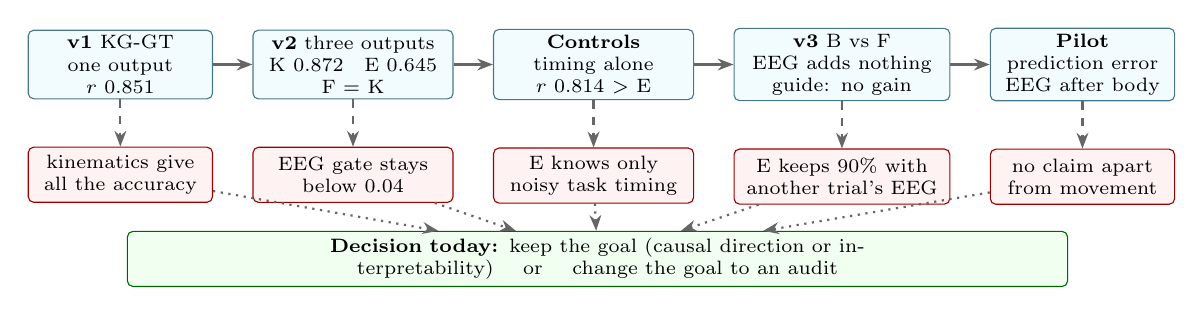
\begin{tikzpicture}[node distance=4mm and 5mm]
    \node[blk,text width=22mm] (v1) {\textbf{v1} KG-GT\\one output\\$r$ 0.851};
    \node[blk,text width=24mm,right=of v1] (v2) {\textbf{v2} three outputs\\K 0.872 \; E 0.645\\F $=$ K};
    \node[blk,text width=24mm,right=of v2] (ctl) {\textbf{Controls}\\timing alone\\$r$ 0.814 $>$ E};
    \node[blk,text width=26mm,right=of ctl] (v3) {\textbf{v3} B vs F\\EEG adds nothing\\guide: no gain};
    \node[blk,text width=22mm,right=of v3] (pe) {\textbf{Pilot}\\prediction error\\EEG after body};
    \foreach \a/\b in {v1/v2,v2/ctl,ctl/v3,v3/pe} \draw[arr] (\a) -- (\b);
    \node[bad,text width=22mm,below=6mm of v1] (q1) {kinematics give\\all the accuracy};
    \node[bad,text width=24mm,below=6mm of v2] (q2) {EEG gate stays\\below 0.04};
    \node[bad,text width=24mm,below=6mm of ctl] (q3) {E knows only\\noisy task timing};
    \node[bad,text width=26mm,below=6mm of v3] (q4) {E keeps 90\% with\\another trial's EEG};
    \node[bad,text width=22mm,below=6mm of pe] (q5) {no claim apart\\from movement};
    \foreach \a/\b in {v1/q1,v2/q2,ctl/q3,v3/q4,pe/q5} \draw[arr,dashed] (\a) -- (\b);
    \node[good,text width=118mm,below=7mm of $(q2)!0.5!(q4)$] (dec) {\textbf{Decision today:} keep the goal (causal direction or interpretability) \quad or \quad change the goal to an audit};
    \foreach \a in {q1,q2,q3,q4,q5} \draw[arr,dotted] (\a) -- (dec);
  \end{tikzpicture}
  \FigCap{Each model was built to answer the doubt left by the one before it.}
\end{frame}

%% =============================================================
\section{v1: one model, one output}
%% =============================================================

\begin{frame}{v1 (KG-GT): Kinematics-Guided Graph Transformer}
  \centering
  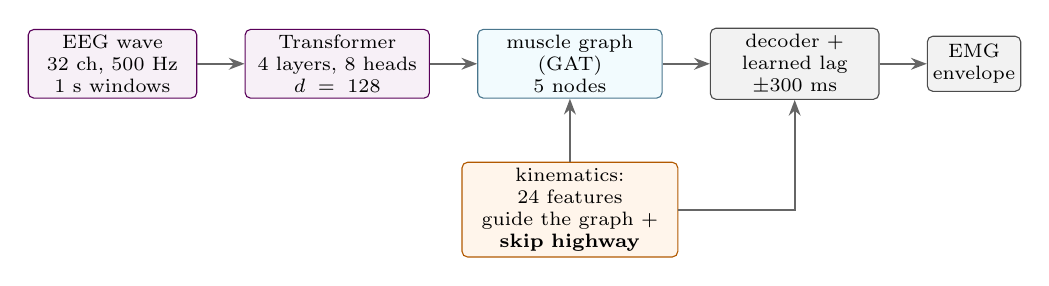
\begin{tikzpicture}[node distance=3mm and 6mm]
    \node[eeg,text width=20mm] (e) {EEG wave\\32 ch, 500 Hz\\1 s windows};
    \node[eeg,text width=22mm,right=of e] (tr) {Transformer\\4 layers, 8 heads\\$d=128$};
    \node[blk,text width=22mm,right=of tr] (g) {muscle graph (GAT)\\5 nodes};
    \node[res,text width=20mm,right=of g] (o) {decoder +\\learned lag\\$\pm$300 ms};
    \node[res,right=of o] (y) {EMG\\envelope};
    \node[kin,text width=26mm,below=8mm of g] (k) {kinematics: 24 features\\guide the graph +\\\textbf{skip highway}};
    \draw[arr] (e)--(tr); \draw[arr] (tr)--(g); \draw[arr] (g)--(o); \draw[arr] (o)--(y);
    \draw[arr] (k)--(g); \draw[arr] (k.east) -| (o.south);
  \end{tikzpicture}

  \medskip
  \begin{columns}[T]
    \column{0.48\linewidth}
    \textbf{Result on test series}
    \begin{itemize}\small
      \item VAF 72.2\%, $r$ 0.851
    \end{itemize}
    \textbf{Input ablation} ($r$, mean of 12)
    \begin{itemize}\small
      \item kinematics set to zero: 0.851 $\to$ \alert{0.035}
      \item EEG swapped between windows: \alert{0.855} (no loss)
    \end{itemize}
    \column{0.48\linewidth}
    \begin{tcolorbox}[notebox,title={What v1 left open}]
      Almost all accuracy comes from kinematics, through the skip highway. With one mixed output there is no way to
      measure what the EEG contributes, or to trace where a prediction comes from.
    \end{tcolorbox}
  \end{columns}
\end{frame}


\begin{frame}{v1 output: one test stretch (P1, test series 4)}
  \begin{columns}[T]
    \column{0.56\linewidth}
    \FigRow{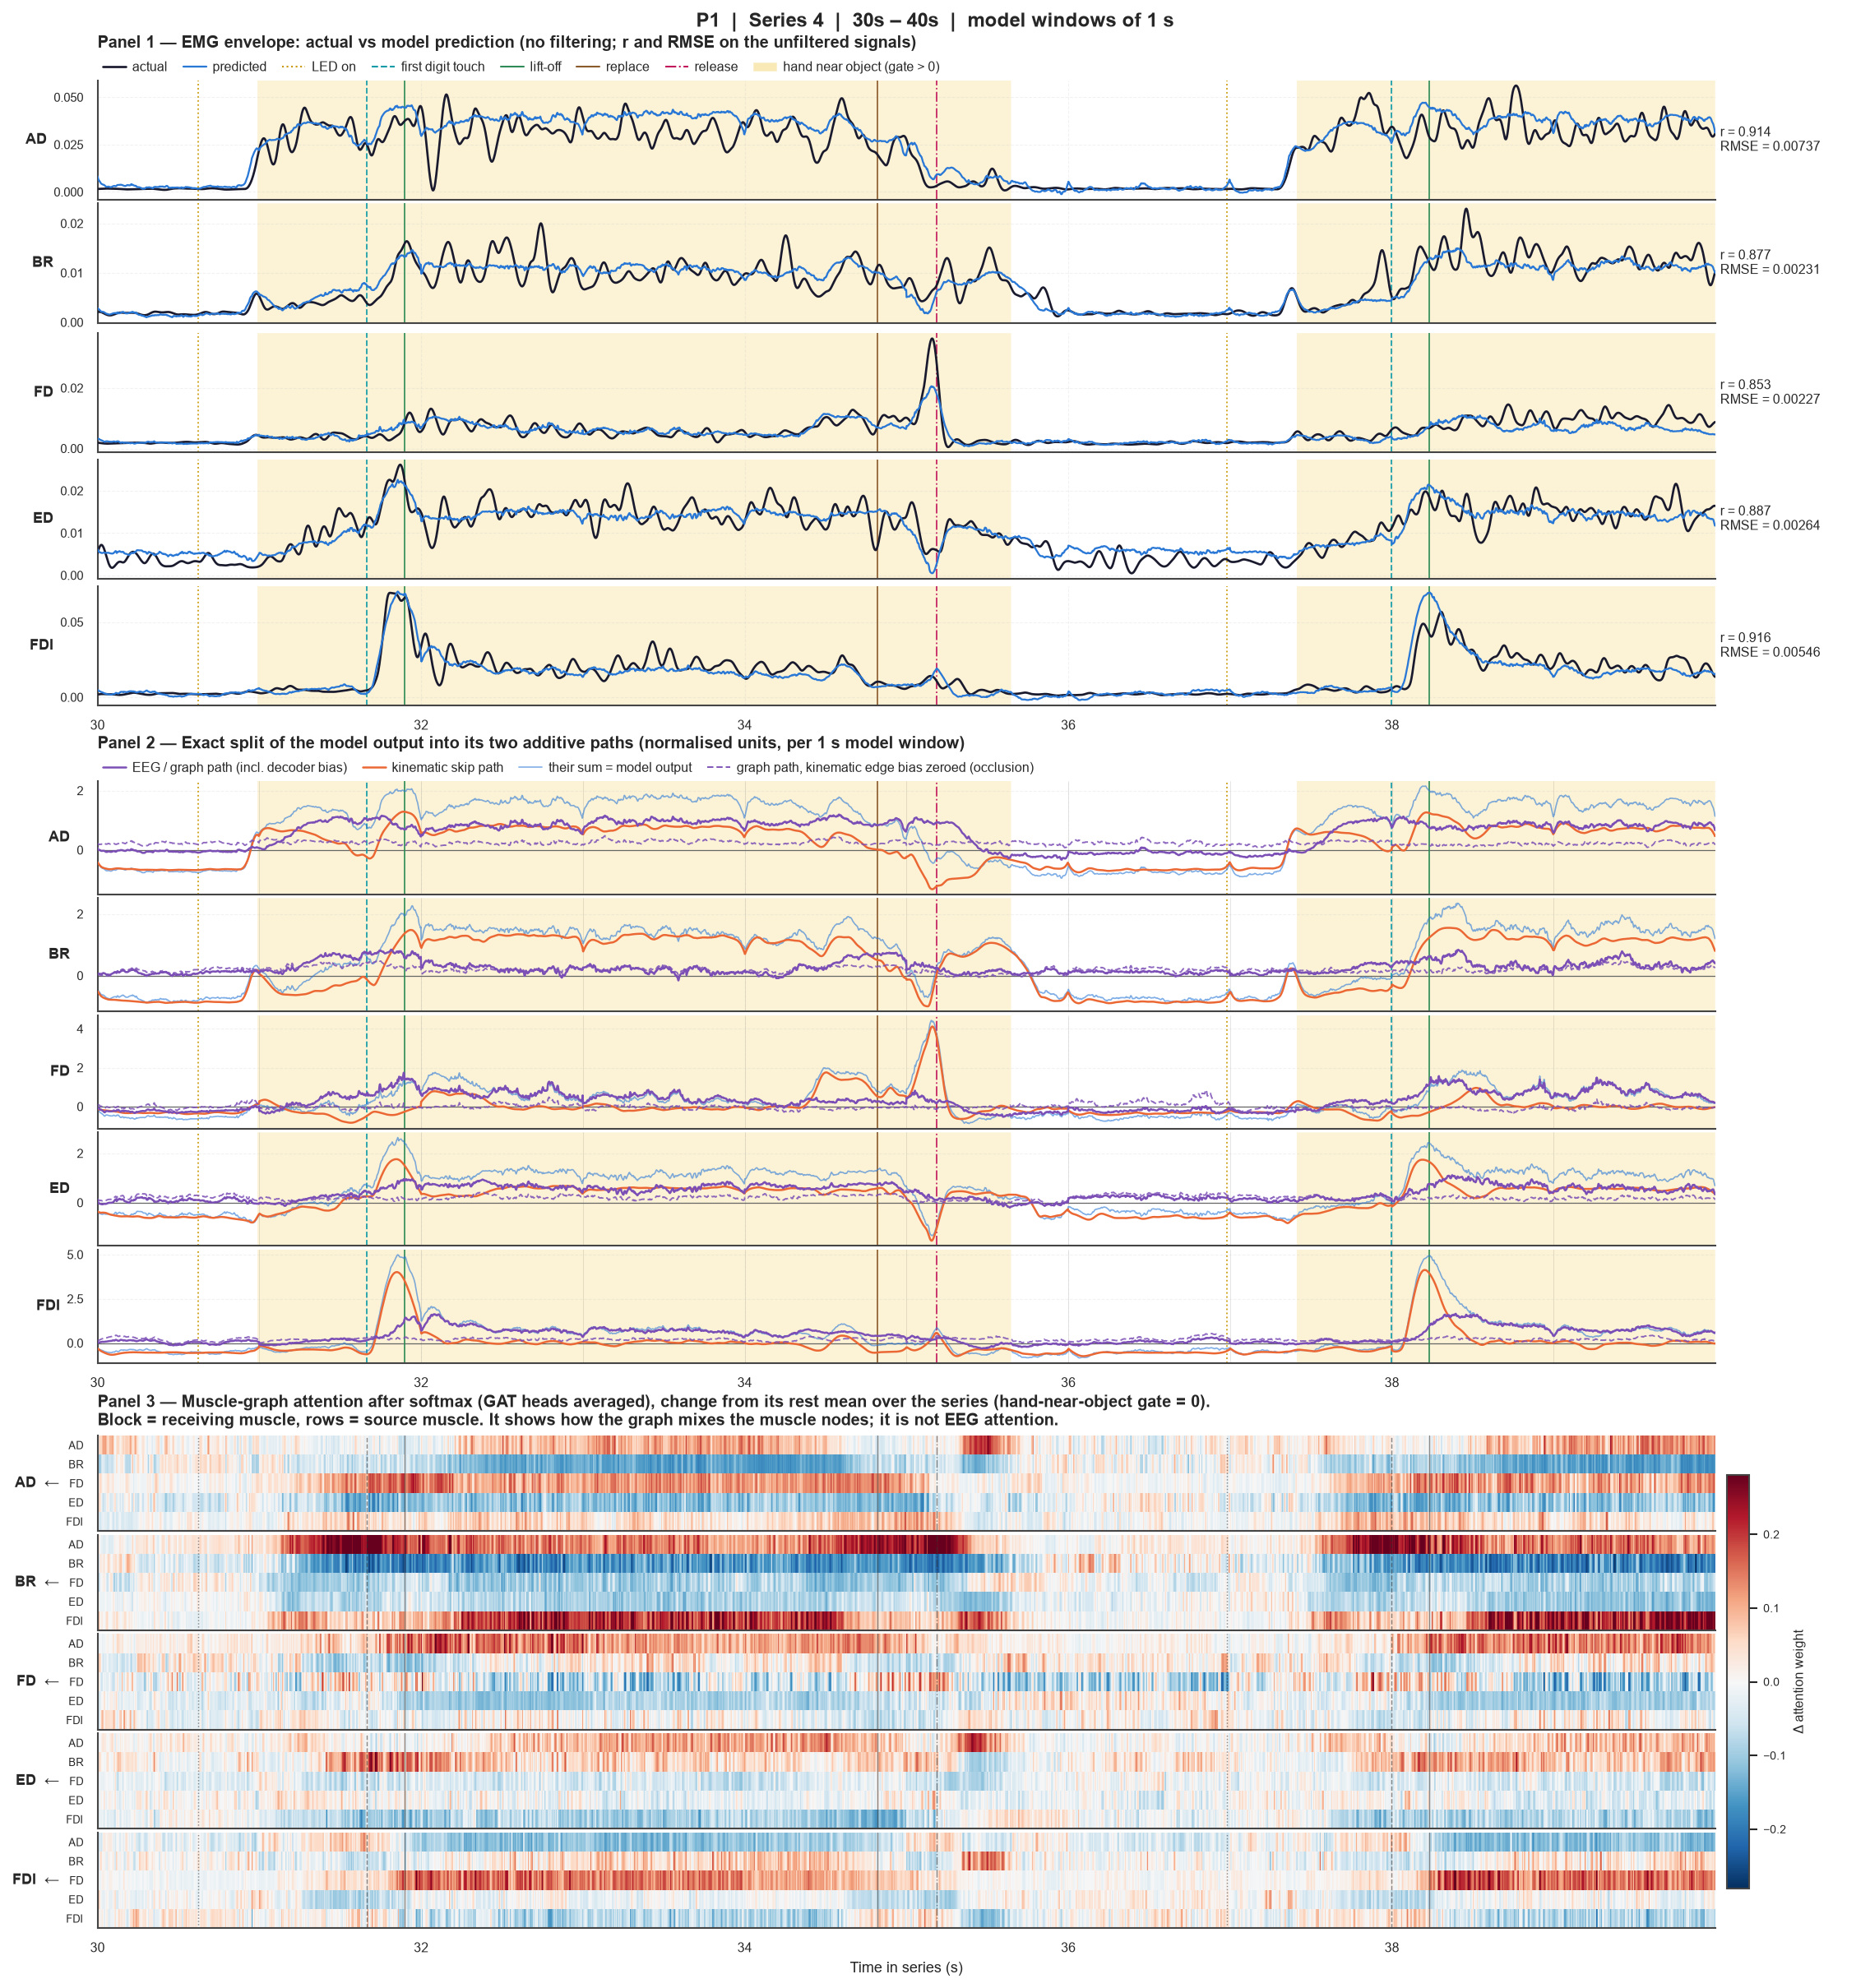
\includegraphics[height=70mm,width=\linewidth,keepaspectratio]{base_triptych_P1.png}}
    \column{0.40\linewidth}
    \textbf{How to read it}
    \begin{itemize}\scriptsize
      \item \textbf{Panel 1:} true envelope (black) and the single prediction (blue), five muscles, 10 s; task events
            as vertical lines; shaded: hand near the object (gate $>0$); $r$ and RMSE per muscle.
      \item \textbf{Panel 2:} exact split of the output into its two additive paths, per 1 s window: EEG/graph path
            (purple), kinematic skip highway (orange), their sum (light blue). Dashed purple: the graph path with
            the \emph{kinematic edge bias} zeroed.
      \item \textbf{Panel 3:} muscle-graph attention after softmax (heads averaged), change from its rest mean;
            block = receiving muscle, rows = source muscle.
    \end{itemize}
    \begin{tcolorbox}[notebox,title={What it shows}]
      The purple ``EEG'' path is as large as the orange one, but it collapses when the kinematic edge bias is zeroed
      (dashed): its size comes from kinematics guiding the graph, not from the EEG. So no panel can show what the EEG
      itself added.
    \end{tcolorbox}
  \end{columns}
\end{frame}

\begin{frame}{v1 tests: input ablation and the residual experiment}
  \begin{columns}[T]
    \column{0.50\linewidth}
    \FigRow{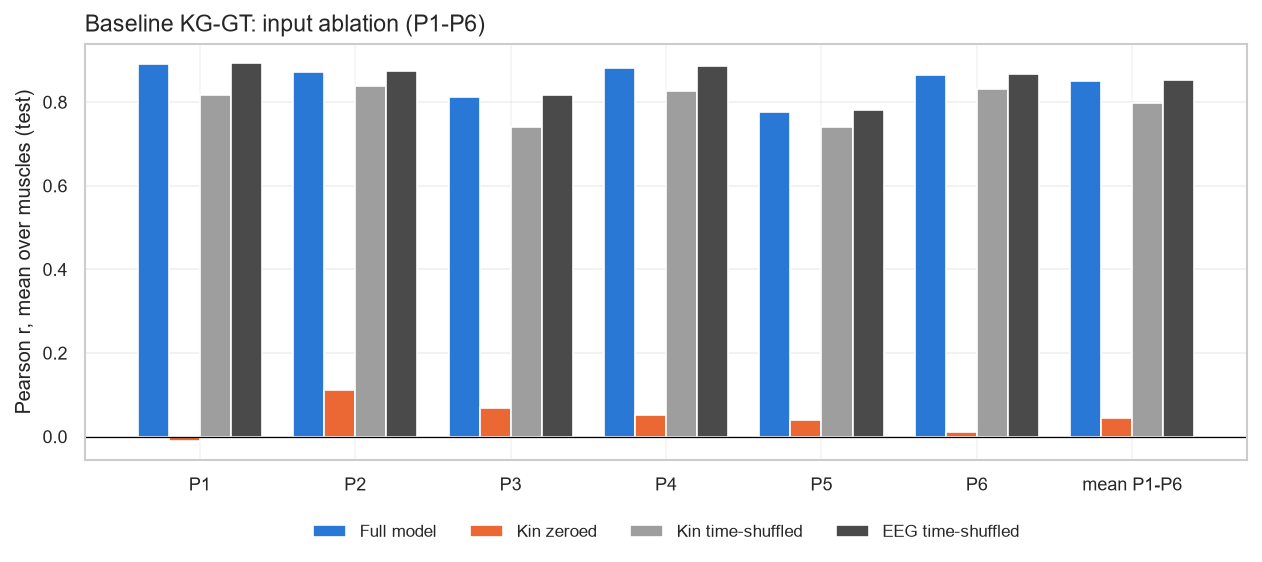
\includegraphics[height=34mm,width=\linewidth,keepaspectratio]{base_ablation.png}}
    \FigCap{Input ablation, P1--P6: full model, kinematics zero, kinematics time-shifted, EEG time-shifted.}
    \begin{itemize}\scriptsize
      \item Kinematics zero: $r$ 0.851 $\to$ 0.035.
      \item EEG swapped: $r$ 0.855, slightly \emph{higher}.
    \end{itemize}
    \column{0.46\linewidth}
    \FigRow{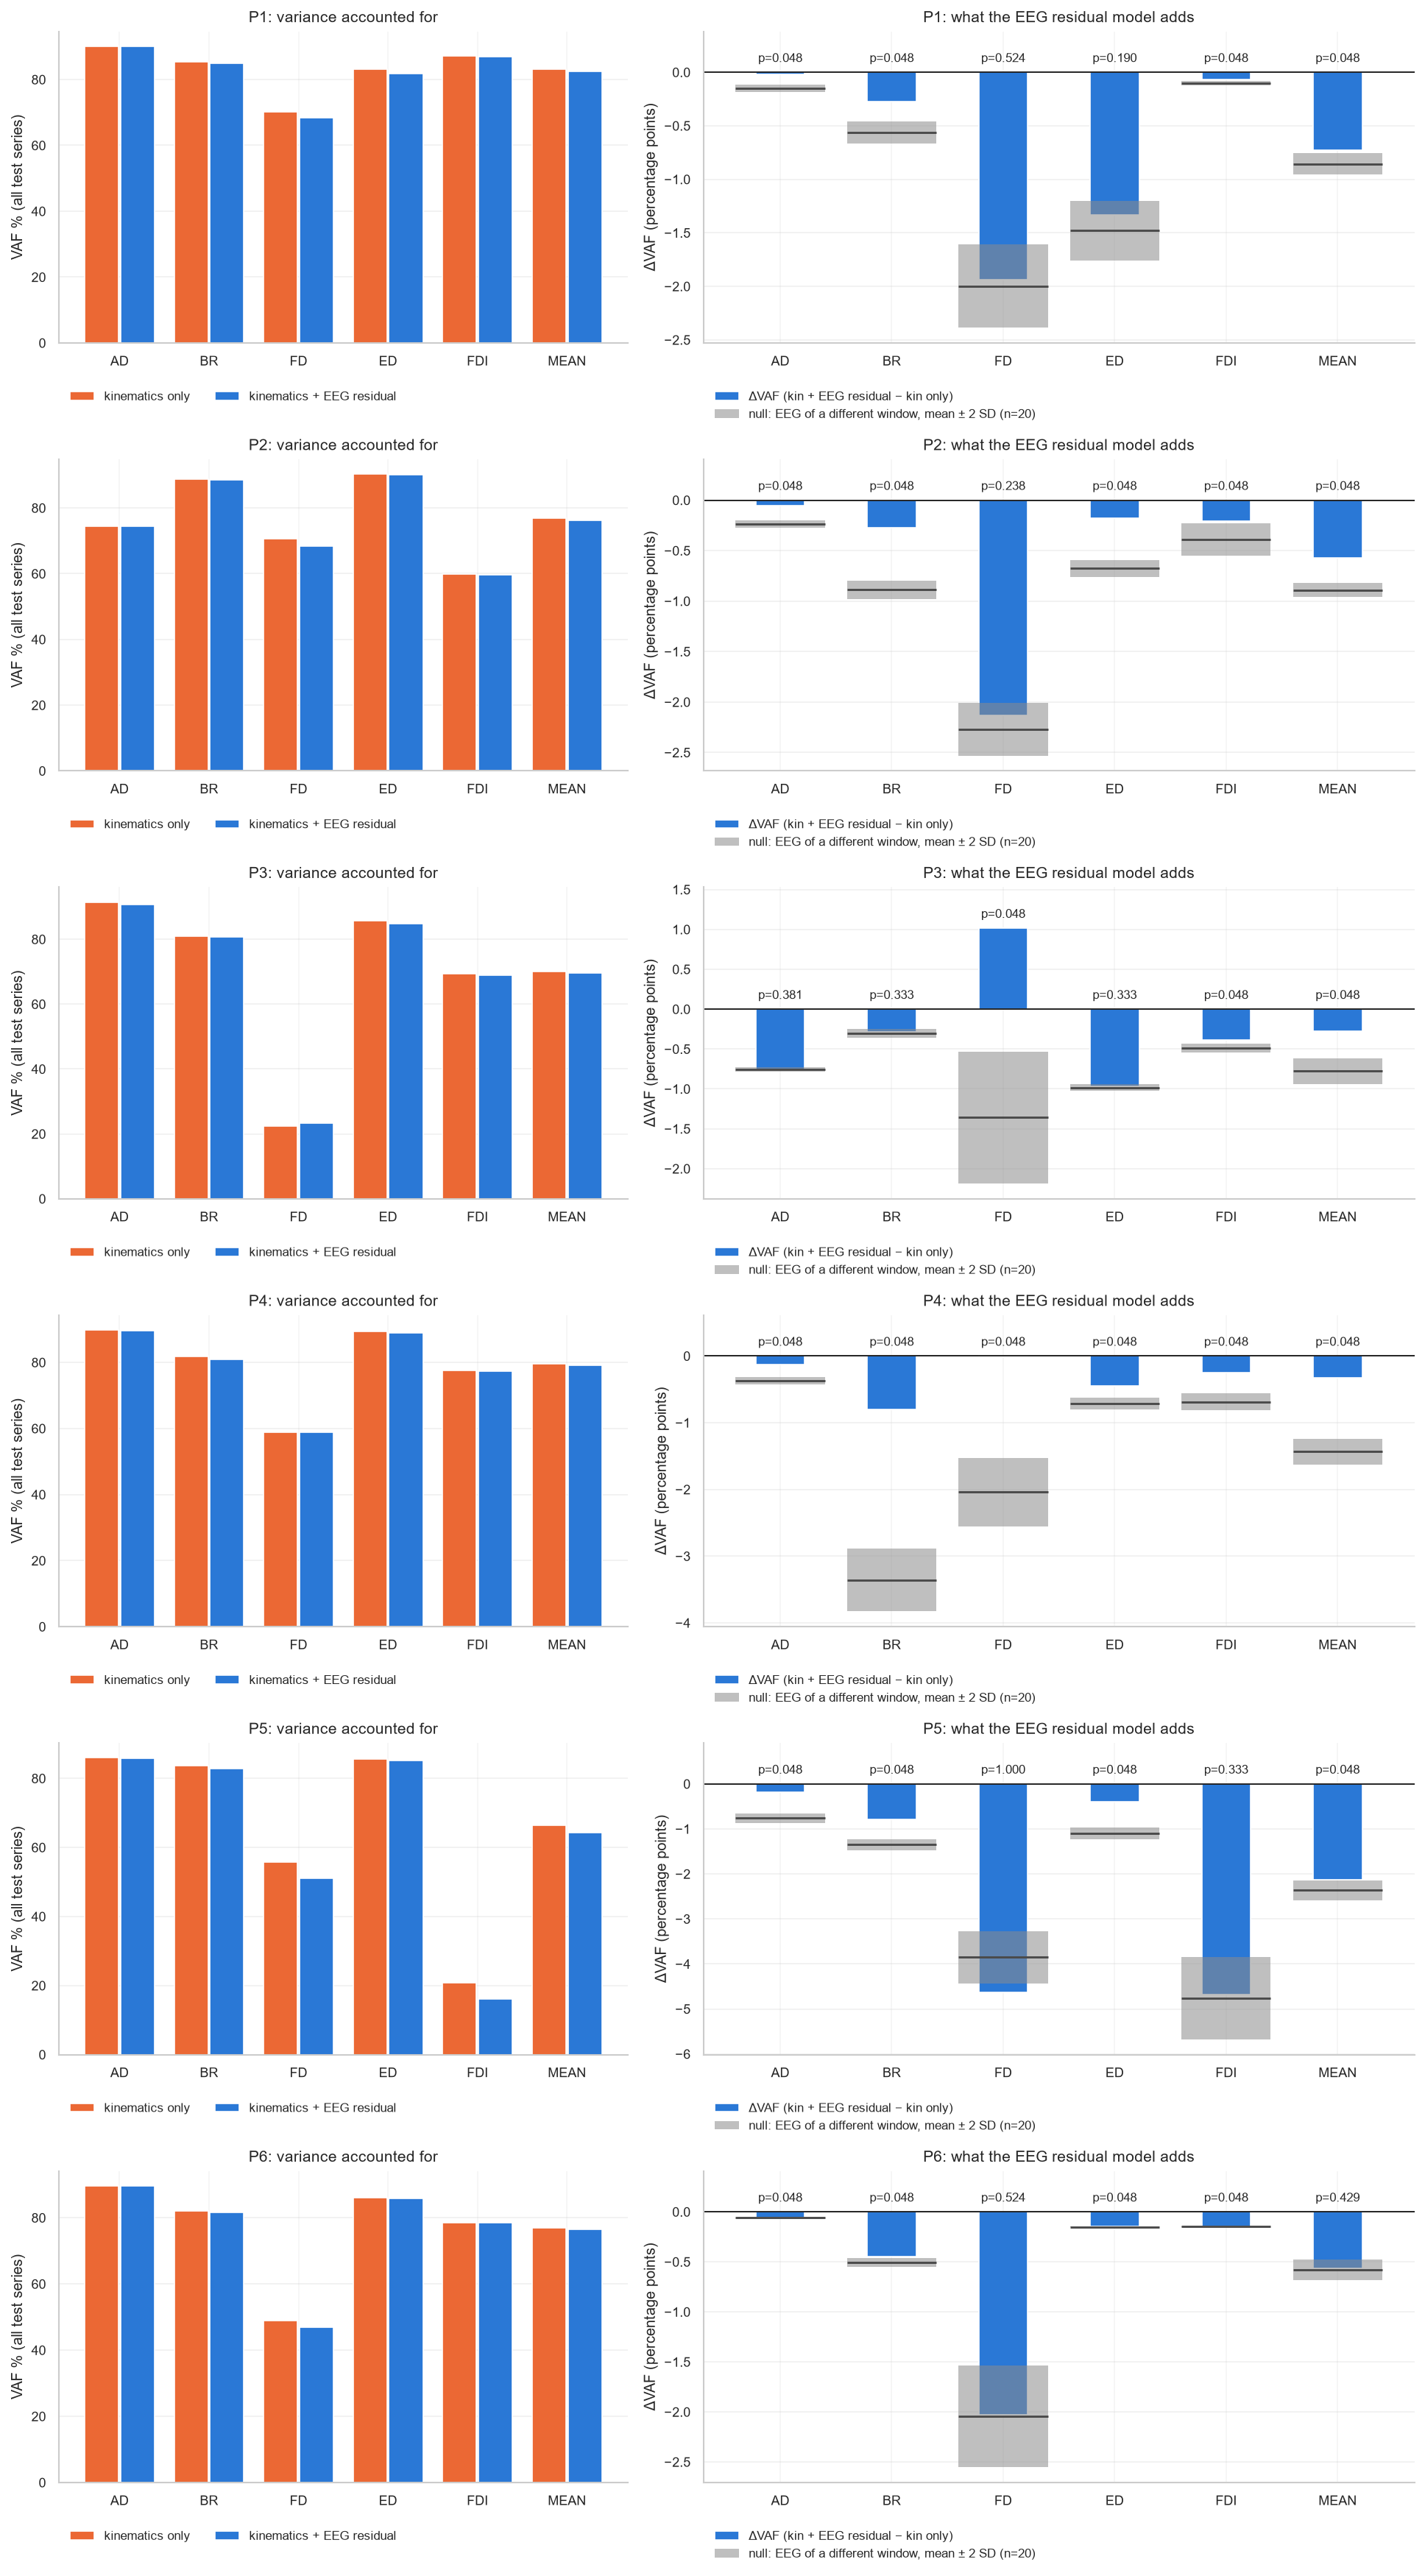
\includegraphics[height=44mm,width=\linewidth,keepaspectratio]{base_residual_dvaf.png}}
    \FigCap{Residual experiment, P1--P6: a kinematics-only model, then EEG fitted on its residual.}
    \begin{itemize}\scriptsize
      \item Kinematics-only model: VAF 75.5\%, above the full v1.
      \item Adding EEG on the residual: $-0.74$ VAF points.
      \item 4 of 60 participant--muscle pairs improve; about 3 are expected by chance.
    \end{itemize}
  \end{columns}
\end{frame}

\begin{frame}{v1 tests: amplitude errors depend on the weight}
  \begin{columns}[T]
    \column{0.40\linewidth}
    \FigRow{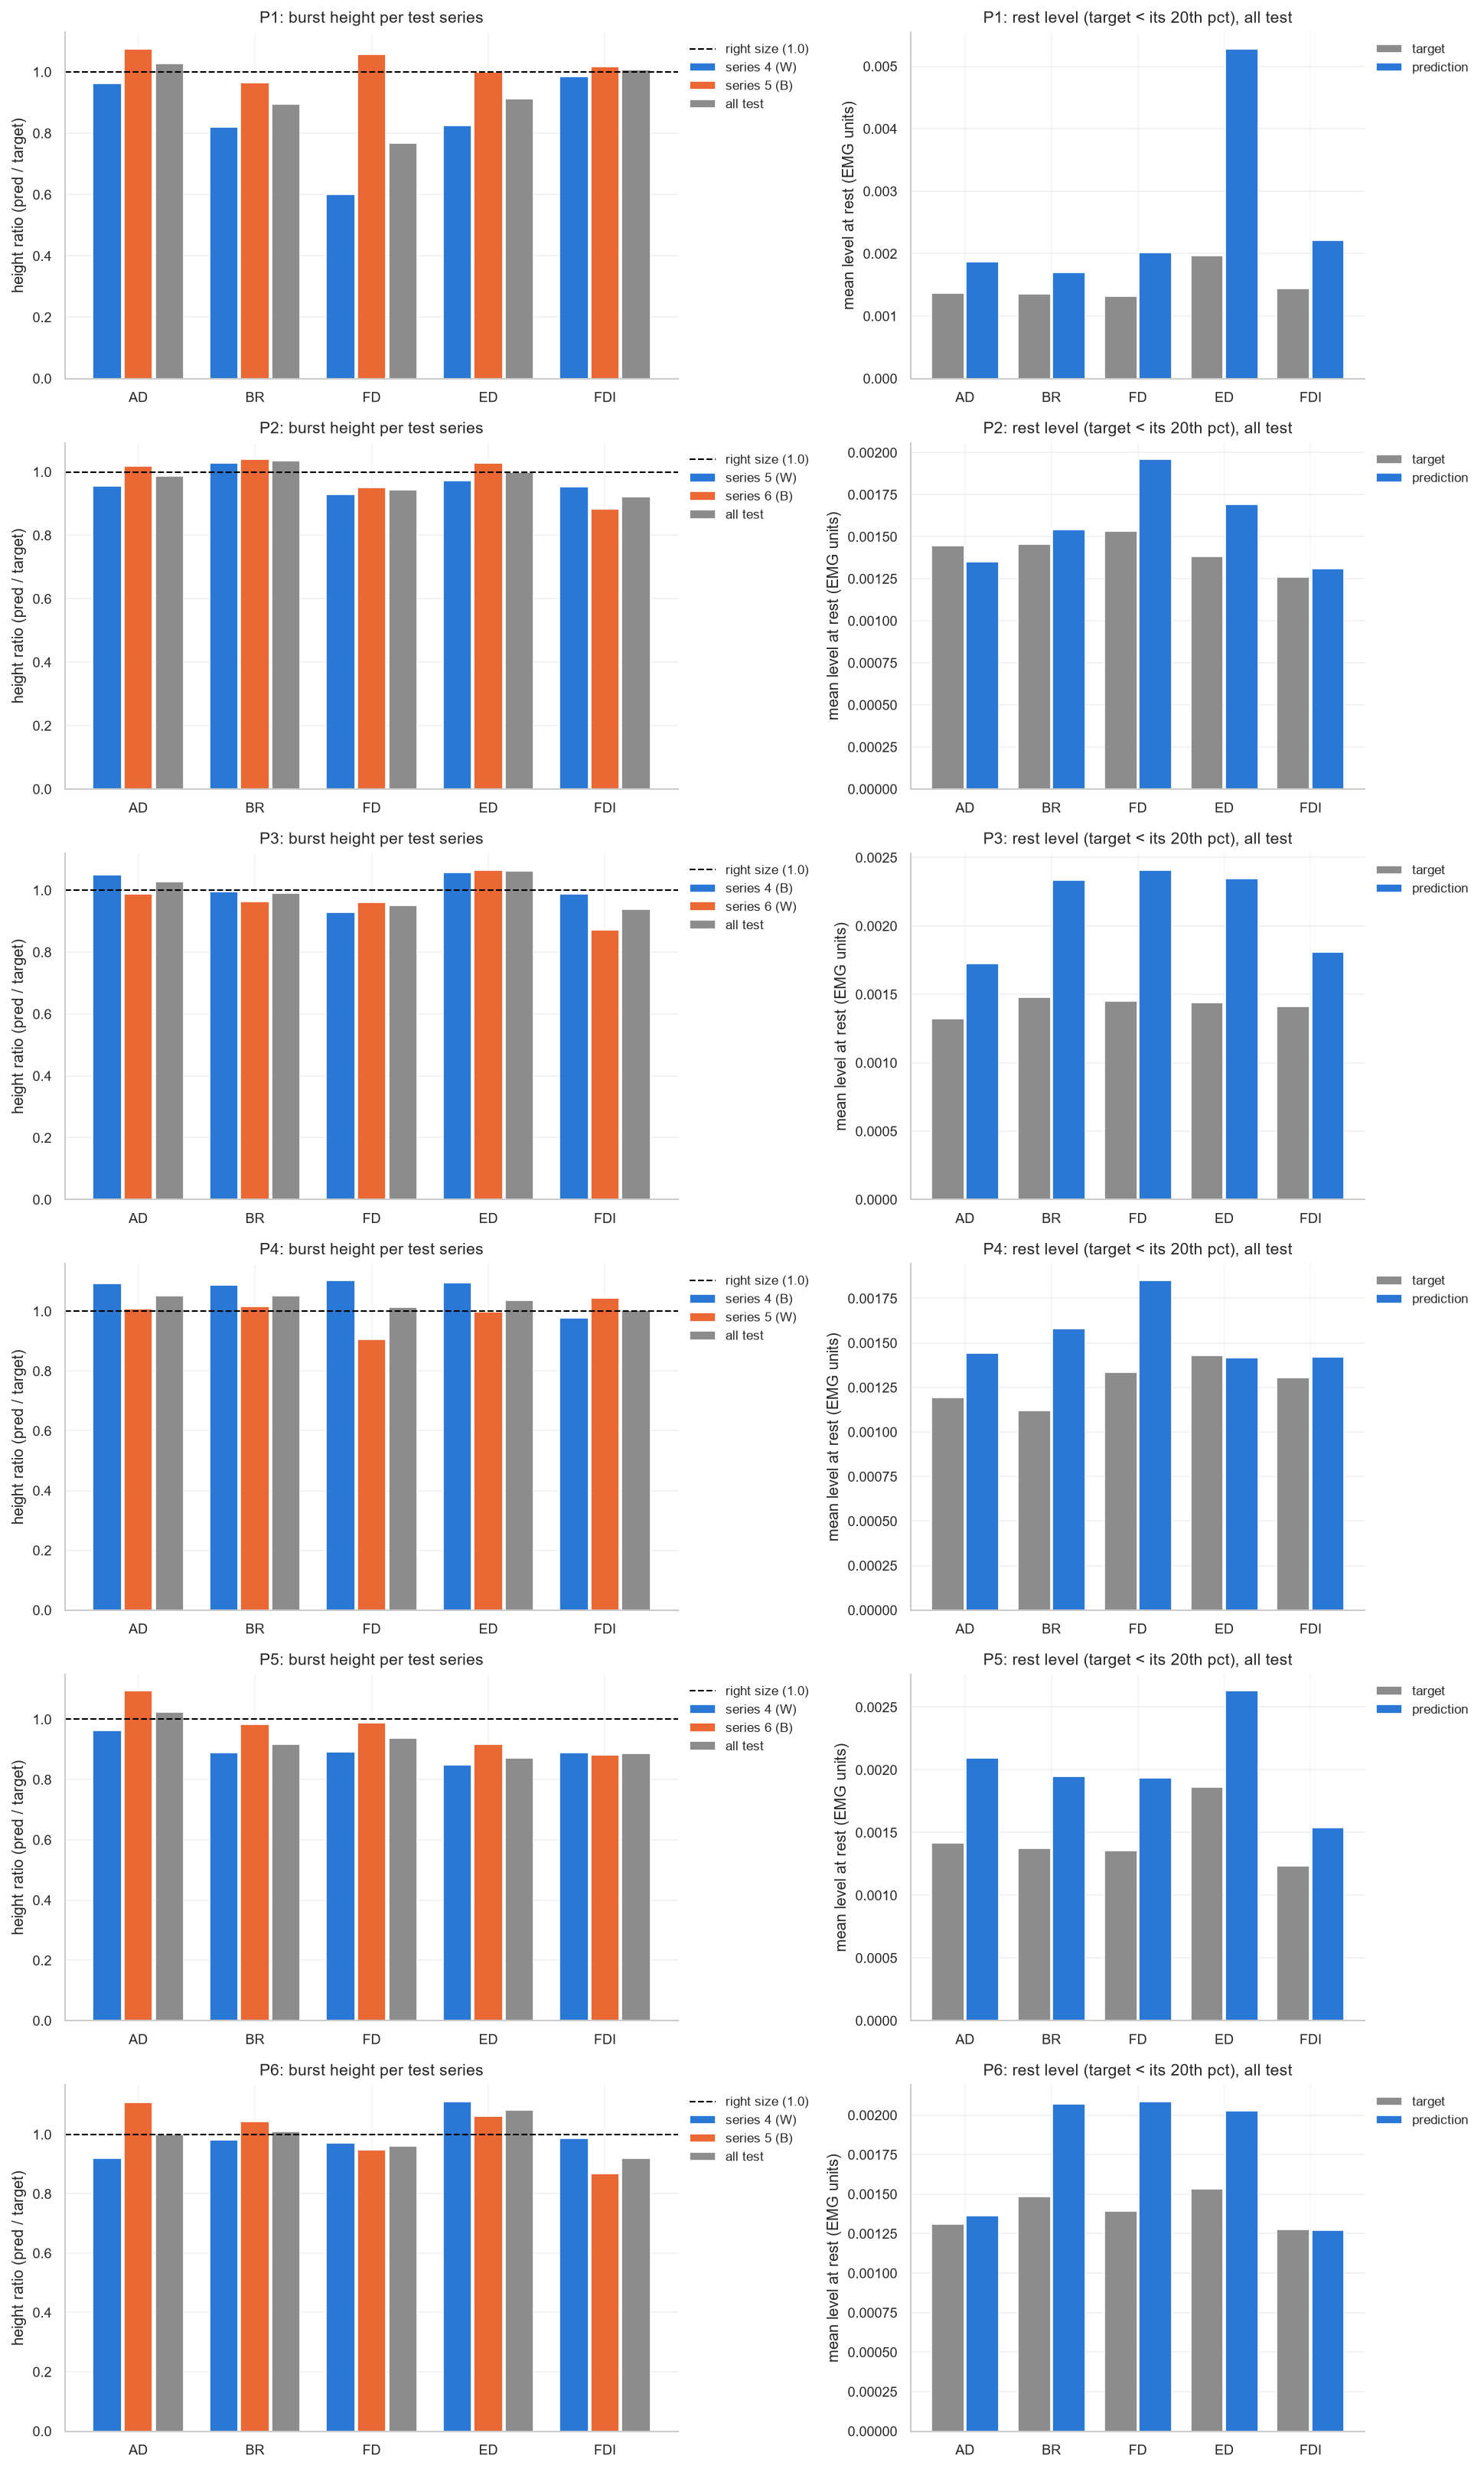
\includegraphics[height=70mm,width=\linewidth,keepaspectratio]{base_magnitude.png}}
    \column{0.56\linewidth}
    \begin{itemize}\scriptsize
      \item \textbf{Height ratio} = mean prediction / mean true envelope during the hold (1 = right level).
      \item Mean height ratio 0.973: the overall level is right.
      \item But errors are one-sided: over-estimates are larger (0.138) than under-estimates (0.089).
      \item Light and medium weights are over-estimated by 4--11\%. When the weight stays the same, the model does not
            follow the small changes of level from one lift to the next (AD: $r\approx0.07$).
      \item The loss had eight terms (peak weighting, costlier under-estimation, a rest term); together they push
            towards over-estimation, and no single term can be blamed.
    \end{itemize}
    \begin{tcolorbox}[notebox,title={What v2 changed because of this}]
      8 s context, lift-history features, a square-root target, a per-hold \emph{lift} term in a 4-term loss, and three
      separate outputs.
    \end{tcolorbox}
  \end{columns}
\end{frame}

%% =============================================================
\section{v2: three outputs}
%% =============================================================

\begin{frame}{v2 preprocessing: 500 Hz cache, then 50 Hz tokens}
  \centering
  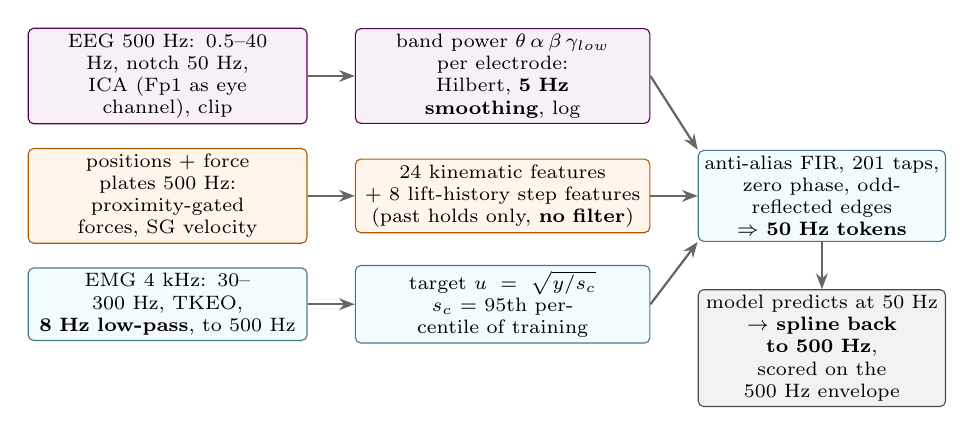
\begin{tikzpicture}[node distance=3mm and 6mm]
    \node[eeg,text width=34mm] (e1) {EEG 500 Hz: 0.5--40 Hz, notch 50 Hz,\\ICA (Fp1 as eye channel), clip};
    \node[eeg,text width=36mm,right=of e1] (e2) {band power $\theta\,\alpha\,\beta\,\gamma_{low}$ per electrode:\\Hilbert, \textbf{5 Hz smoothing}, log};
    \node[kin,text width=34mm,below=of e1] (k1) {positions + force plates 500 Hz:\\proximity-gated forces, SG velocity};
    \node[kin,text width=36mm,right=of k1] (k2) {24 kinematic features\\+ 8 lift-history step features\\(past holds only, \textbf{no filter})};
    \node[blk,text width=34mm,below=of k1] (m1) {EMG 4 kHz: 30--300 Hz, TKEO,\\\textbf{8 Hz low-pass}, to 500 Hz};
    \node[blk,text width=36mm,right=of m1] (m2) {target $u=\sqrt{y/s_c}$\\$s_c$ = 95th percentile of training};
    \node[blk,text width=30mm,right=of k2] (tok) {anti-alias FIR, 201 taps,\\zero phase, odd-reflected edges\\$\Rightarrow$ \textbf{50 Hz tokens}};
    \node[res,text width=30mm,below=of tok,yshift=-3mm] (ev) {model predicts at 50 Hz\\$\to$ \textbf{spline back to 500 Hz},\\scored on the 500 Hz envelope};
    \draw[arr] (e1)--(e2); \draw[arr] (k1)--(k2); \draw[arr] (m1)--(m2);
    \draw[arr] (e2.east) -- (tok.north west); \draw[arr] (k2)--(tok); \draw[arr] (m2.east) -- (tok.south west);
    \draw[arr] (tok)--(ev);
  \end{tikzpicture}
  \FigCap{Rule: every filter runs on the whole series at 500 Hz before the rate is reduced; windows are cut afterwards.}
  \Verify{\scriptsize ICA uses Fp1 as the eye channel (no EOG in the data); causal EMG filters add about 60 ms of lag to the target. Acceptable?}
\end{frame}

\begin{frame}{Main question 1: is down- and up-sampling allowed in v2?}
  \begin{columns}[T]
    \column{0.55\linewidth}
    \textbf{Our argument: no information is lost.}
    \begin{itemize}\scriptsize
      \item 50 Hz tokens keep everything below 25 Hz (Nyquist).
      \item Every signal is already band-limited far below that:\\
        EMG envelope: 8 Hz low-pass \quad EEG band power: 5 Hz smoothing\\
        hand movement: a few Hz \quad lift history: step functions
      \item Anti-alias FIR, zero phase, so no time shift; edges handled by odd reflection.
      \item Step features are sub-sampled \emph{without} a filter, so a step is never seen early (no leak from the future).
      \item The score is computed after spline up-sampling against the original 500 Hz envelope, so any loss would show
            in the numbers.
    \end{itemize}
    \column{0.41\linewidth}
    \begin{tcolorbox}[stagebox,title={Direct check (v3, E0, 12 participants)}]
      \centering\scriptsize
      \begin{tabular}{lcc}
        \toprule
        scored at & $r$ & VAF \\
        \midrule
        500 Hz (after up-sampling) & 0.6328 & 36.13 \\
        50 Hz (token rate) & 0.6326 & 36.11 \\
        \bottomrule
      \end{tabular}
    \end{tcolorbox}
    \vspace{2pt}
    \begin{tcolorbox}[notebox,title={What the token rate does give up}]
      The raw EEG wave and its phase are not seen, only band-power envelopes. A gamma oscillation enters as its slow
      power, not as a 30--40 Hz wave.
    \end{tcolorbox}
  \end{columns}
  \Verify{\scriptsize Is this argument enough for a paper, or should the model also be trained at 500 Hz once as a control? Is using only band-power envelopes (no raw EEG phase) a limitation reviewers will raise?}
\end{frame}

\begin{frame}{v2 architecture: K, E and a gated F}
  \centering
  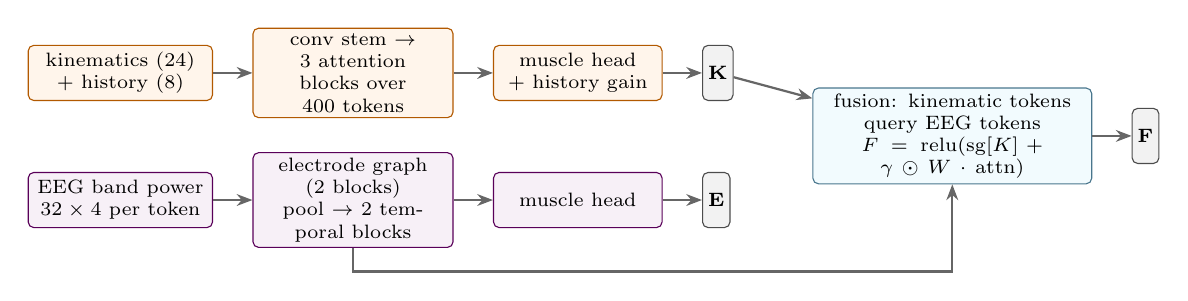
\begin{tikzpicture}[node distance=3mm and 5mm]
    \node[kin,text width=22mm] (ki) {kinematics (24)\\+ history (8)};
    \node[kin,text width=24mm,right=of ki] (ks) {conv stem $\to$ 3 attention\\blocks over 400 tokens};
    \node[kin,text width=20mm,right=of ks] (km) {muscle head\\+ history gain};
    \node[res,right=of km] (K) {\textbf{K}};
    \node[eeg,text width=22mm,below=9mm of ki] (ei) {EEG band power\\$32\times4$ per token};
    \node[eeg,text width=24mm,right=of ei] (es) {electrode graph (2 blocks)\\pool $\to$ 2 temporal blocks};
    \node[eeg,text width=20mm,right=of es] (em) {muscle head};
    \node[res,right=of em] (E) {\textbf{E}};
    \node[blk,text width=34mm,right=10mm of K,yshift=-8mm] (fu) {fusion: kinematic tokens\\query EEG tokens\\$F=\mathrm{relu}(\mathrm{sg}[K]+\gamma\odot W\cdot\mathrm{attn})$};
    \node[res,right=of fu] (F) {\textbf{F}};
    \draw[arr] (ki)--(ks); \draw[arr] (ks)--(km); \draw[arr] (km)--(K);
    \draw[arr] (ei)--(es); \draw[arr] (es)--(em); \draw[arr] (em)--(E);
    \draw[arr] (K)--(fu); \draw[arr] (es.south) |- ++(0,-3mm) -| (fu.south); \draw[arr] (fu)--(F);
  \end{tikzpicture}

  \smallskip
  \begin{columns}[T]
    \column{0.48\linewidth}
    \begin{itemize}\scriptsize
      \item One mixing rule per block: information moves only through attention, so every output can be traced back
            through all layers.
      \item Stop-gradient: K learns only from its own error.
      \item $\gamma$ starts at 0, no weight decay: if EEG is useless, $F=K$.
      \item 337,712 parameters.
    \end{itemize}
    \column{0.48\linewidth}
    \begin{tcolorbox}[notebox,title={Loss, the same for K, E and F (square-root domain)}]
      $L_o=\mathrm{Huber}+0.3\,(1-\mathrm{CCC})+0.5\,\text{lift mean}+0.1\,\text{diff}$, \quad $L=L_K+L_E+L_F$
    \end{tcolorbox}
  \end{columns}
\end{frame}

\begin{frame}{v2 training, step by step}
  \centering
  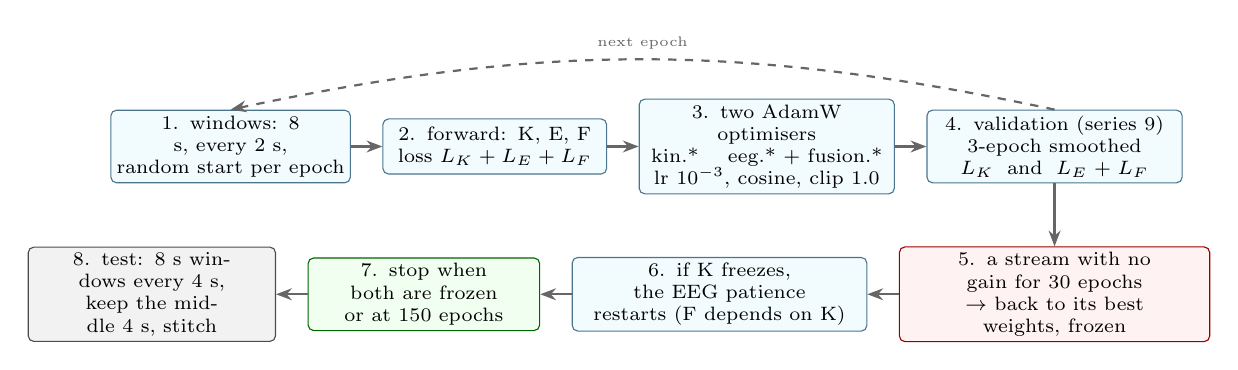
\begin{tikzpicture}[node distance=3mm and 4mm]
    \node[blk,text width=29mm] (w) {1. windows: 8 s, every 2 s,\\random start per epoch};
    \node[blk,text width=27mm,right=of w] (f) {2. forward: K, E, F\\loss $L_K+L_E+L_F$};
    \node[blk,text width=31mm,right=of f] (o) {3. two AdamW optimisers\\kin.* \quad eeg.* + fusion.*\\lr $10^{-3}$, cosine, clip 1.0};
    \node[blk,text width=31mm,right=of o] (v) {4. validation (series 9)\\3-epoch smoothed\\$L_K$ \;and\; $L_E+L_F$};
    \node[bad,text width=38mm,below=8mm of v] (fr) {5. a stream with no gain for 30 epochs\\$\to$ back to its best weights, frozen};
    \node[blk,text width=36mm,left=of fr] (re) {6. if K freezes, the EEG patience\\restarts (F depends on K)};
    \node[good,text width=28mm,left=of re] (st) {7. stop when both are frozen\\or at 150 epochs};
    \node[res,text width=30mm,left=of st] (te) {8. test: 8 s windows every 4 s,\\keep the middle 4 s, stitch};
    \draw[arr] (w)--(f); \draw[arr] (f)--(o); \draw[arr] (o)--(v); \draw[arr] (v)--(fr);
    \draw[arr] (fr)--(re); \draw[arr] (re)--(st); \draw[arr] (st)--(te);
    \draw[arr,dashed] (v.north) to[bend right=12] node[above,font=\tiny]{next epoch} (w.north);
  \end{tikzpicture}
  \FigCap{One model per participant. Batch 32, weight decay 0.01, 5 warm-up epochs, full precision.}
  \Verify{\scriptsize Is per-stream freezing a fair way to train K and E together, or should K and E be trained as two separate models?}
\end{frame}

\begin{frame}{v2 training curves: per-stream freezing in practice (P1)}
  \FigRow{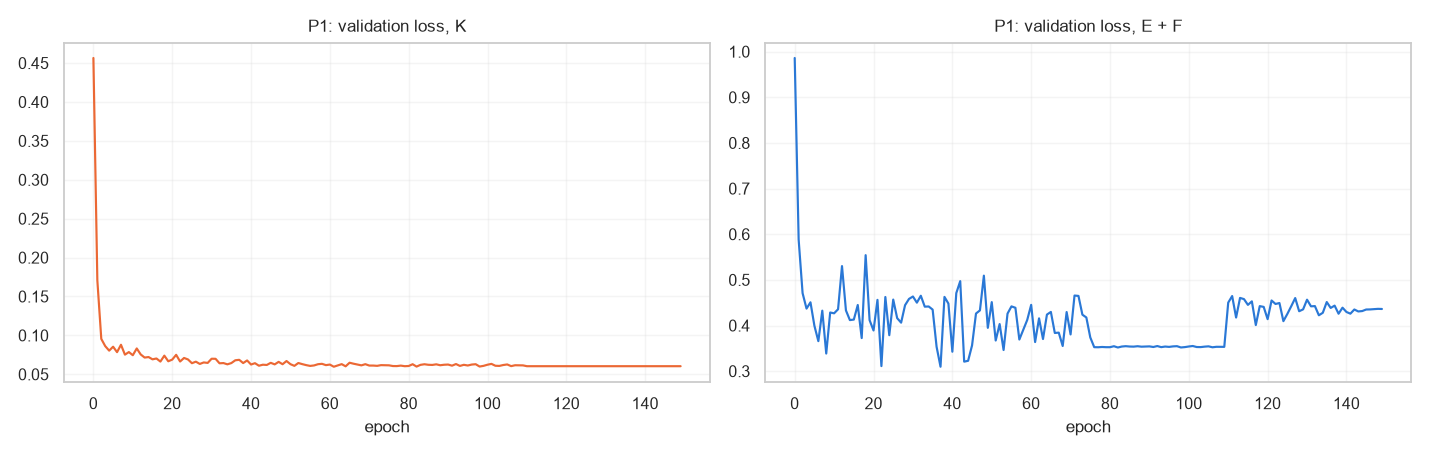
\includegraphics[width=\textwidth,height=48mm,keepaspectratio]{v2_history_P1.png}}
  \FigCap{Validation loss during training. Left: K. Right: E + F.}
  \begin{itemize}\small
    \item K reached its best at epoch 80 and was frozen at epoch 110 (30 epochs without gain).
    \item The EEG stream and the fusion kept training until epoch 150.
    \item Every participant gets its own model; the best epoch of each stream is restored before testing.
  \end{itemize}
\end{frame}

\begin{frame}{v2 results}
  \begin{columns}[T]
    \column{0.47\linewidth}
    \centering\small
    \begin{tabular}{lcc}
      \toprule
      output & VAF (\%) & $r$ \\
      \midrule
      v1 (KG-GT) & 72.2 & 0.851 \\
      \textbf{K} (kinematics + history) & \textbf{75.8} & \textbf{0.872} \\
      \textbf{E} (EEG only) & --- & \textbf{0.645} \\
      \textbf{F} (K + EEG) & 75.9 & $\approx$ K \\
      \bottomrule
    \end{tabular}
    \begin{itemize}\scriptsize
      \item K beats v1 in all 12 participants.
      \item E passes the time-shift null in all 12.
      \item Largest $|\gamma|$ per participant: 0.01--0.04.
      \item Residual test, without the fusion module: EEG predicts K's error with $r\approx0.07$
            (significant in 10 of 12), worth less than 0.5 VAF points.
    \end{itemize}
    \column{0.50\linewidth}
    \begin{tcolorbox}[notebox,title={Interpretability of v2}]
      Attention rollout, attention flow, gradient-weighted rollout and gradient$\times$input, checked with deletion and
      weight-shuffle tests. The group EEG map of E is focused on \textbf{C3 and CP1} and prefers the \textbf{beta}
      band, which is the expected motor-cortex pattern.
    \end{tcolorbox}
    \vspace{2pt}
    \begin{tcolorbox}[askbox,title={Doubt this raised}]
      \scriptsize E reaches 0.645 alone, but adds almost nothing to K. Is E reading motor commands, or only the clock of the task?
    \end{tcolorbox}
  \end{columns}
\end{frame}


\begin{frame}{v2 outputs on the test series: K, E and F}
  \begin{columns}[T]
    \column{0.49\linewidth}
    \FigRow{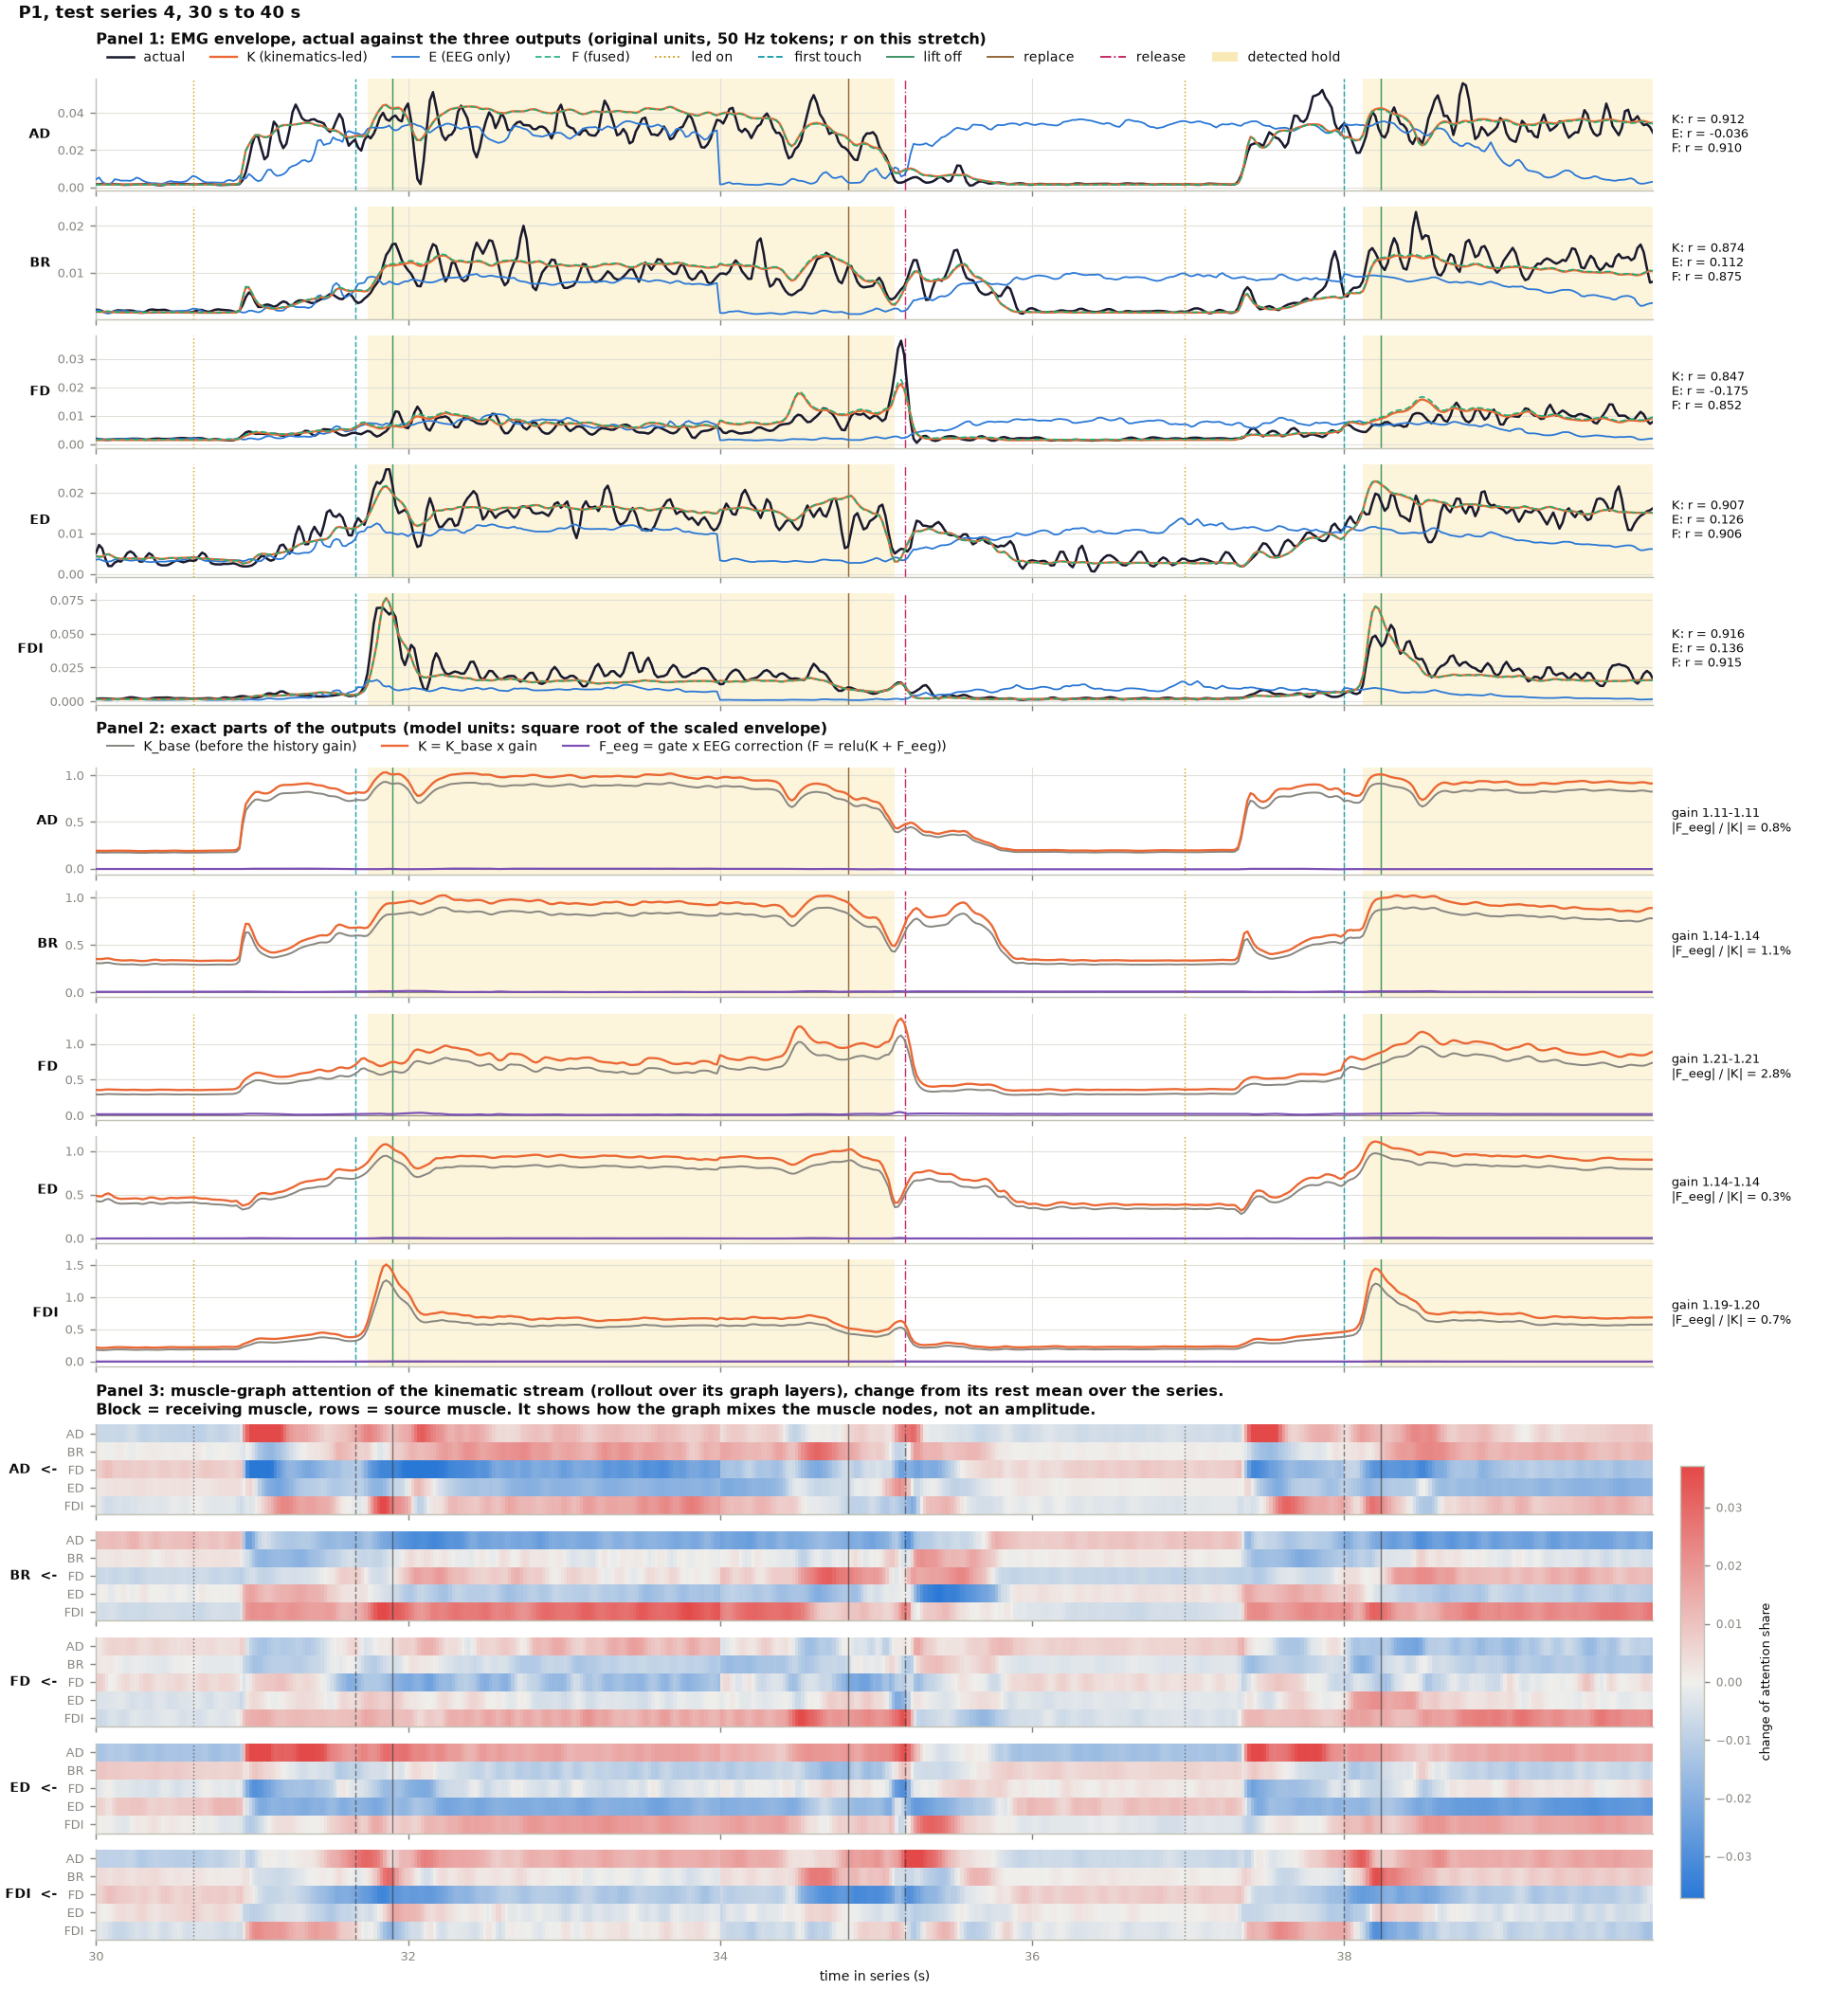
\includegraphics[height=66mm,width=\linewidth,keepaspectratio]{trip_P1_S04.png}}
    \FigCap{P1, test series 4, 30--40 s.}
    \column{0.49\linewidth}
    \FigRow{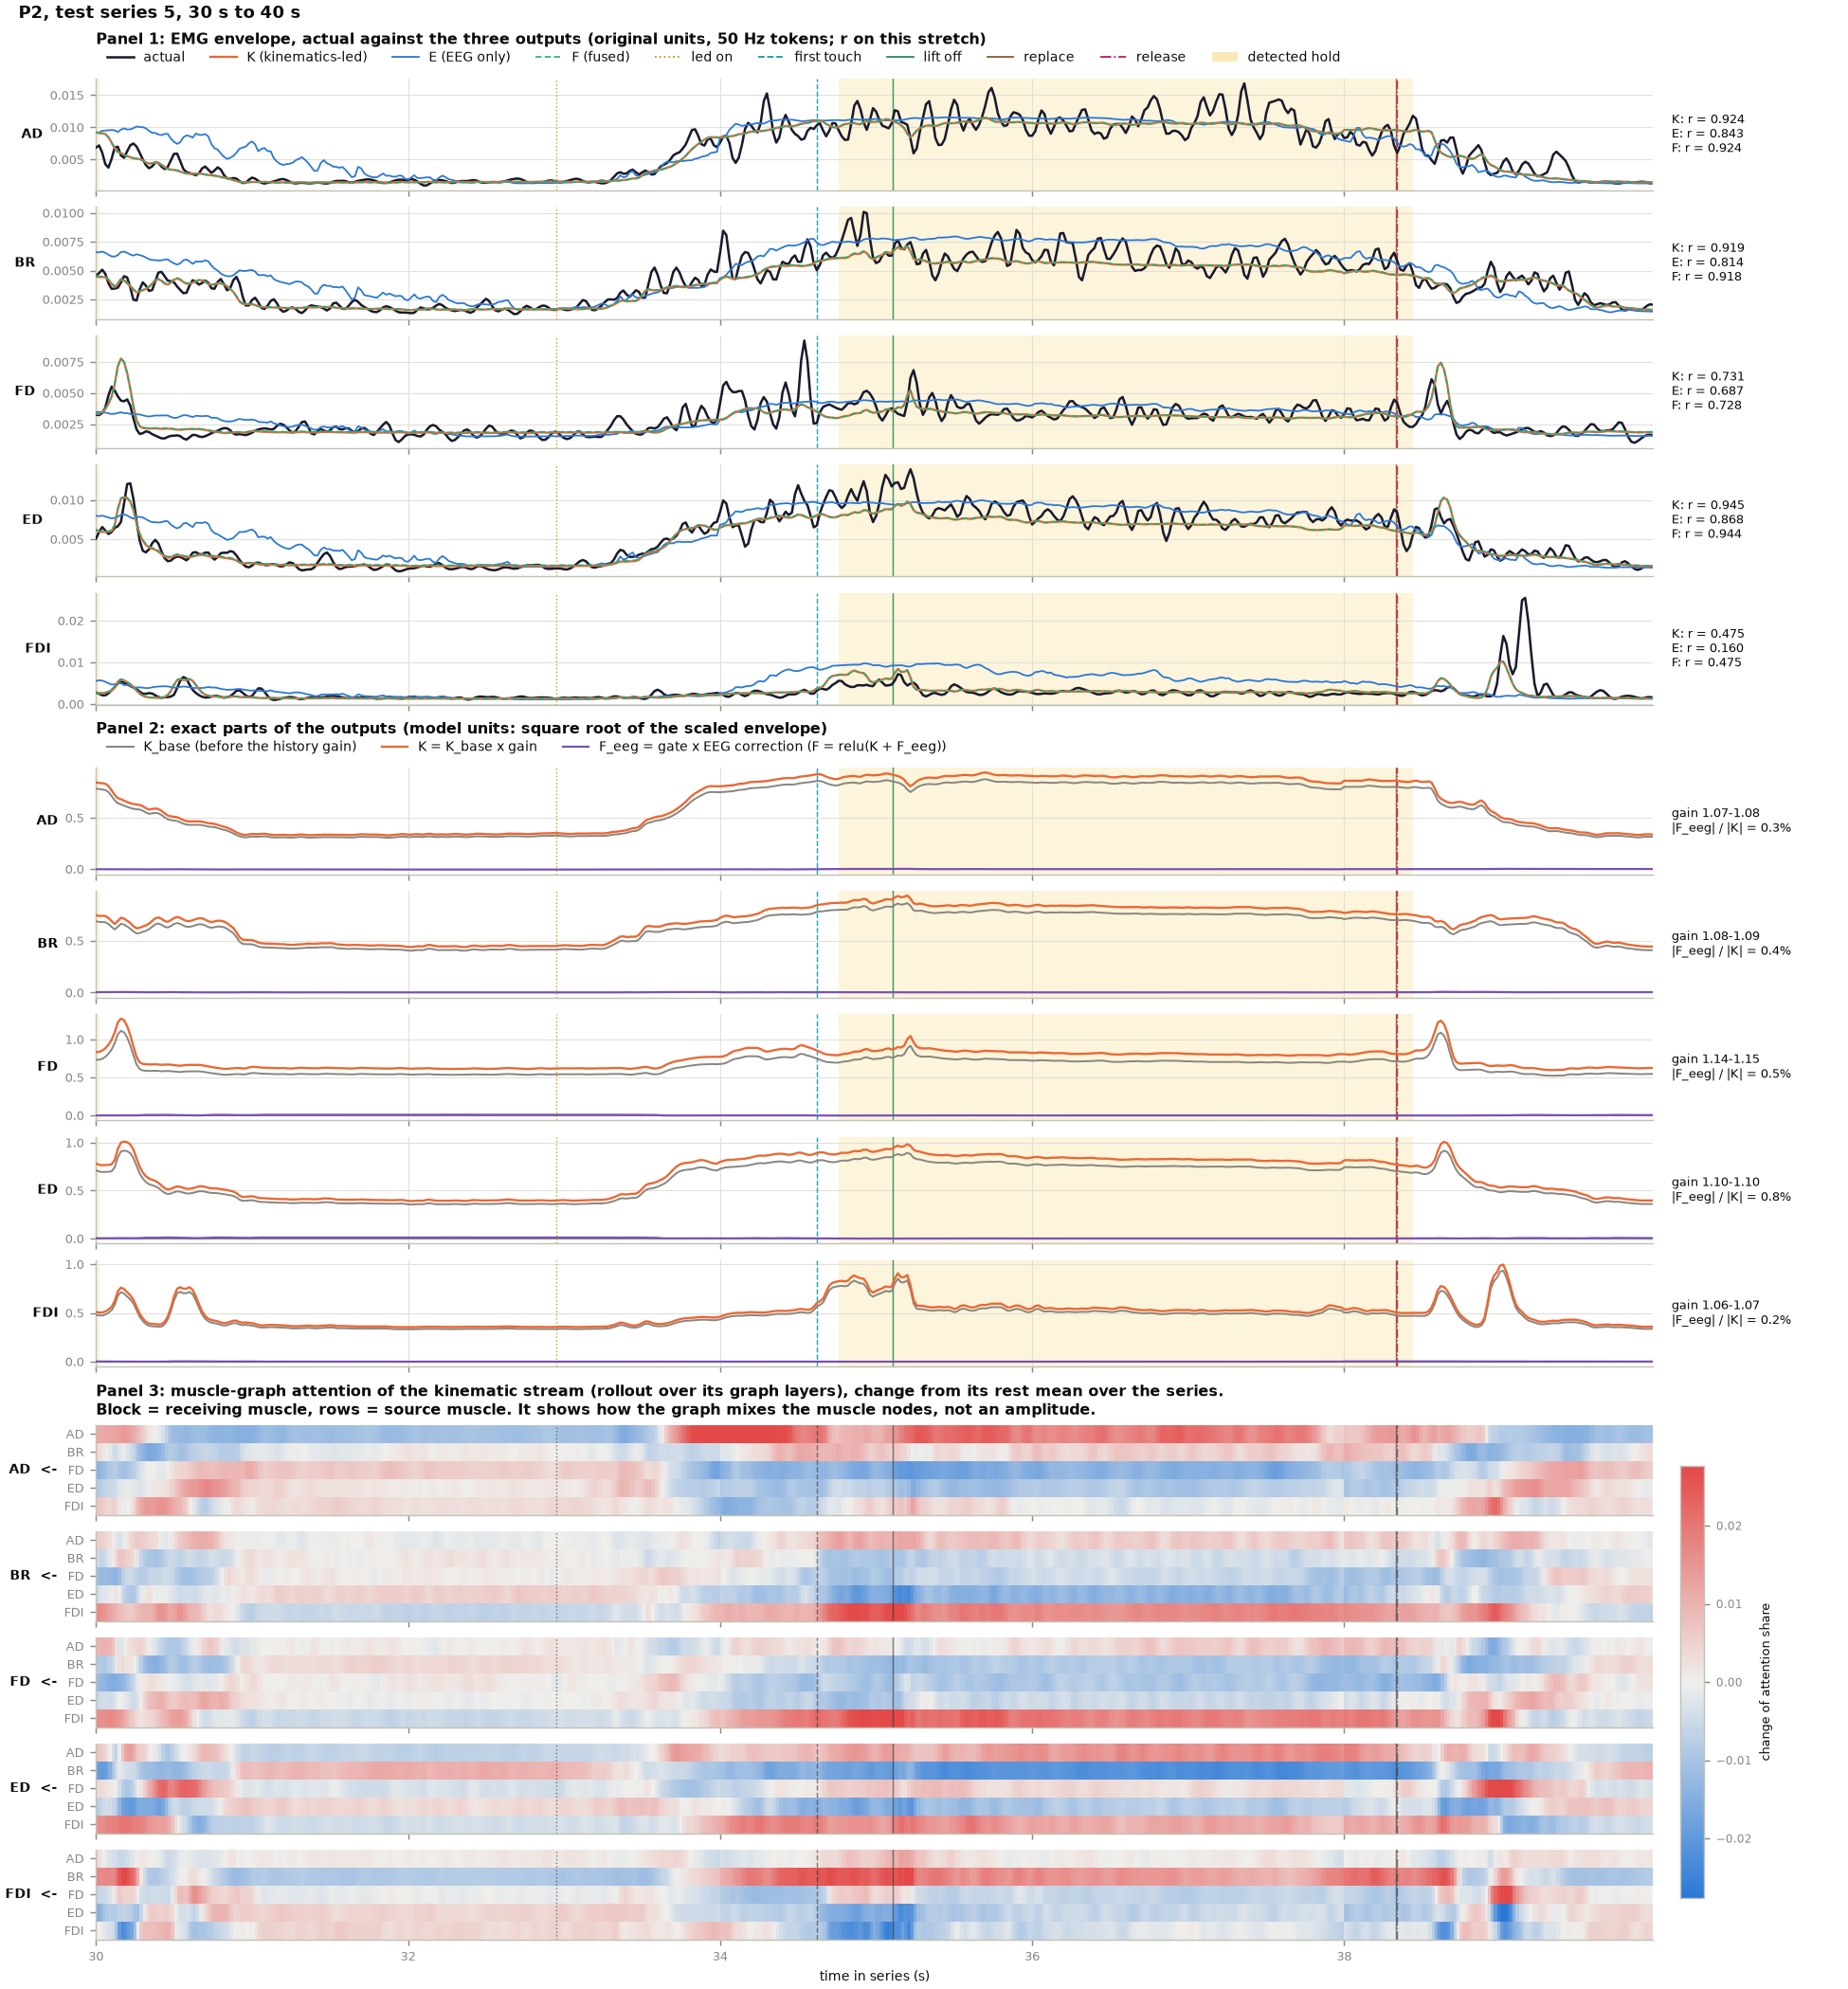
\includegraphics[height=66mm,width=\linewidth,keepaspectratio]{trip_P2_S05.png}}
    \FigCap{P2, test series 5, 30--40 s.}
  \end{columns}
\end{frame}

\begin{frame}{How to read a v2 triptych}
  \begin{columns}[T]
    \column{0.44\linewidth}
    \FigRow{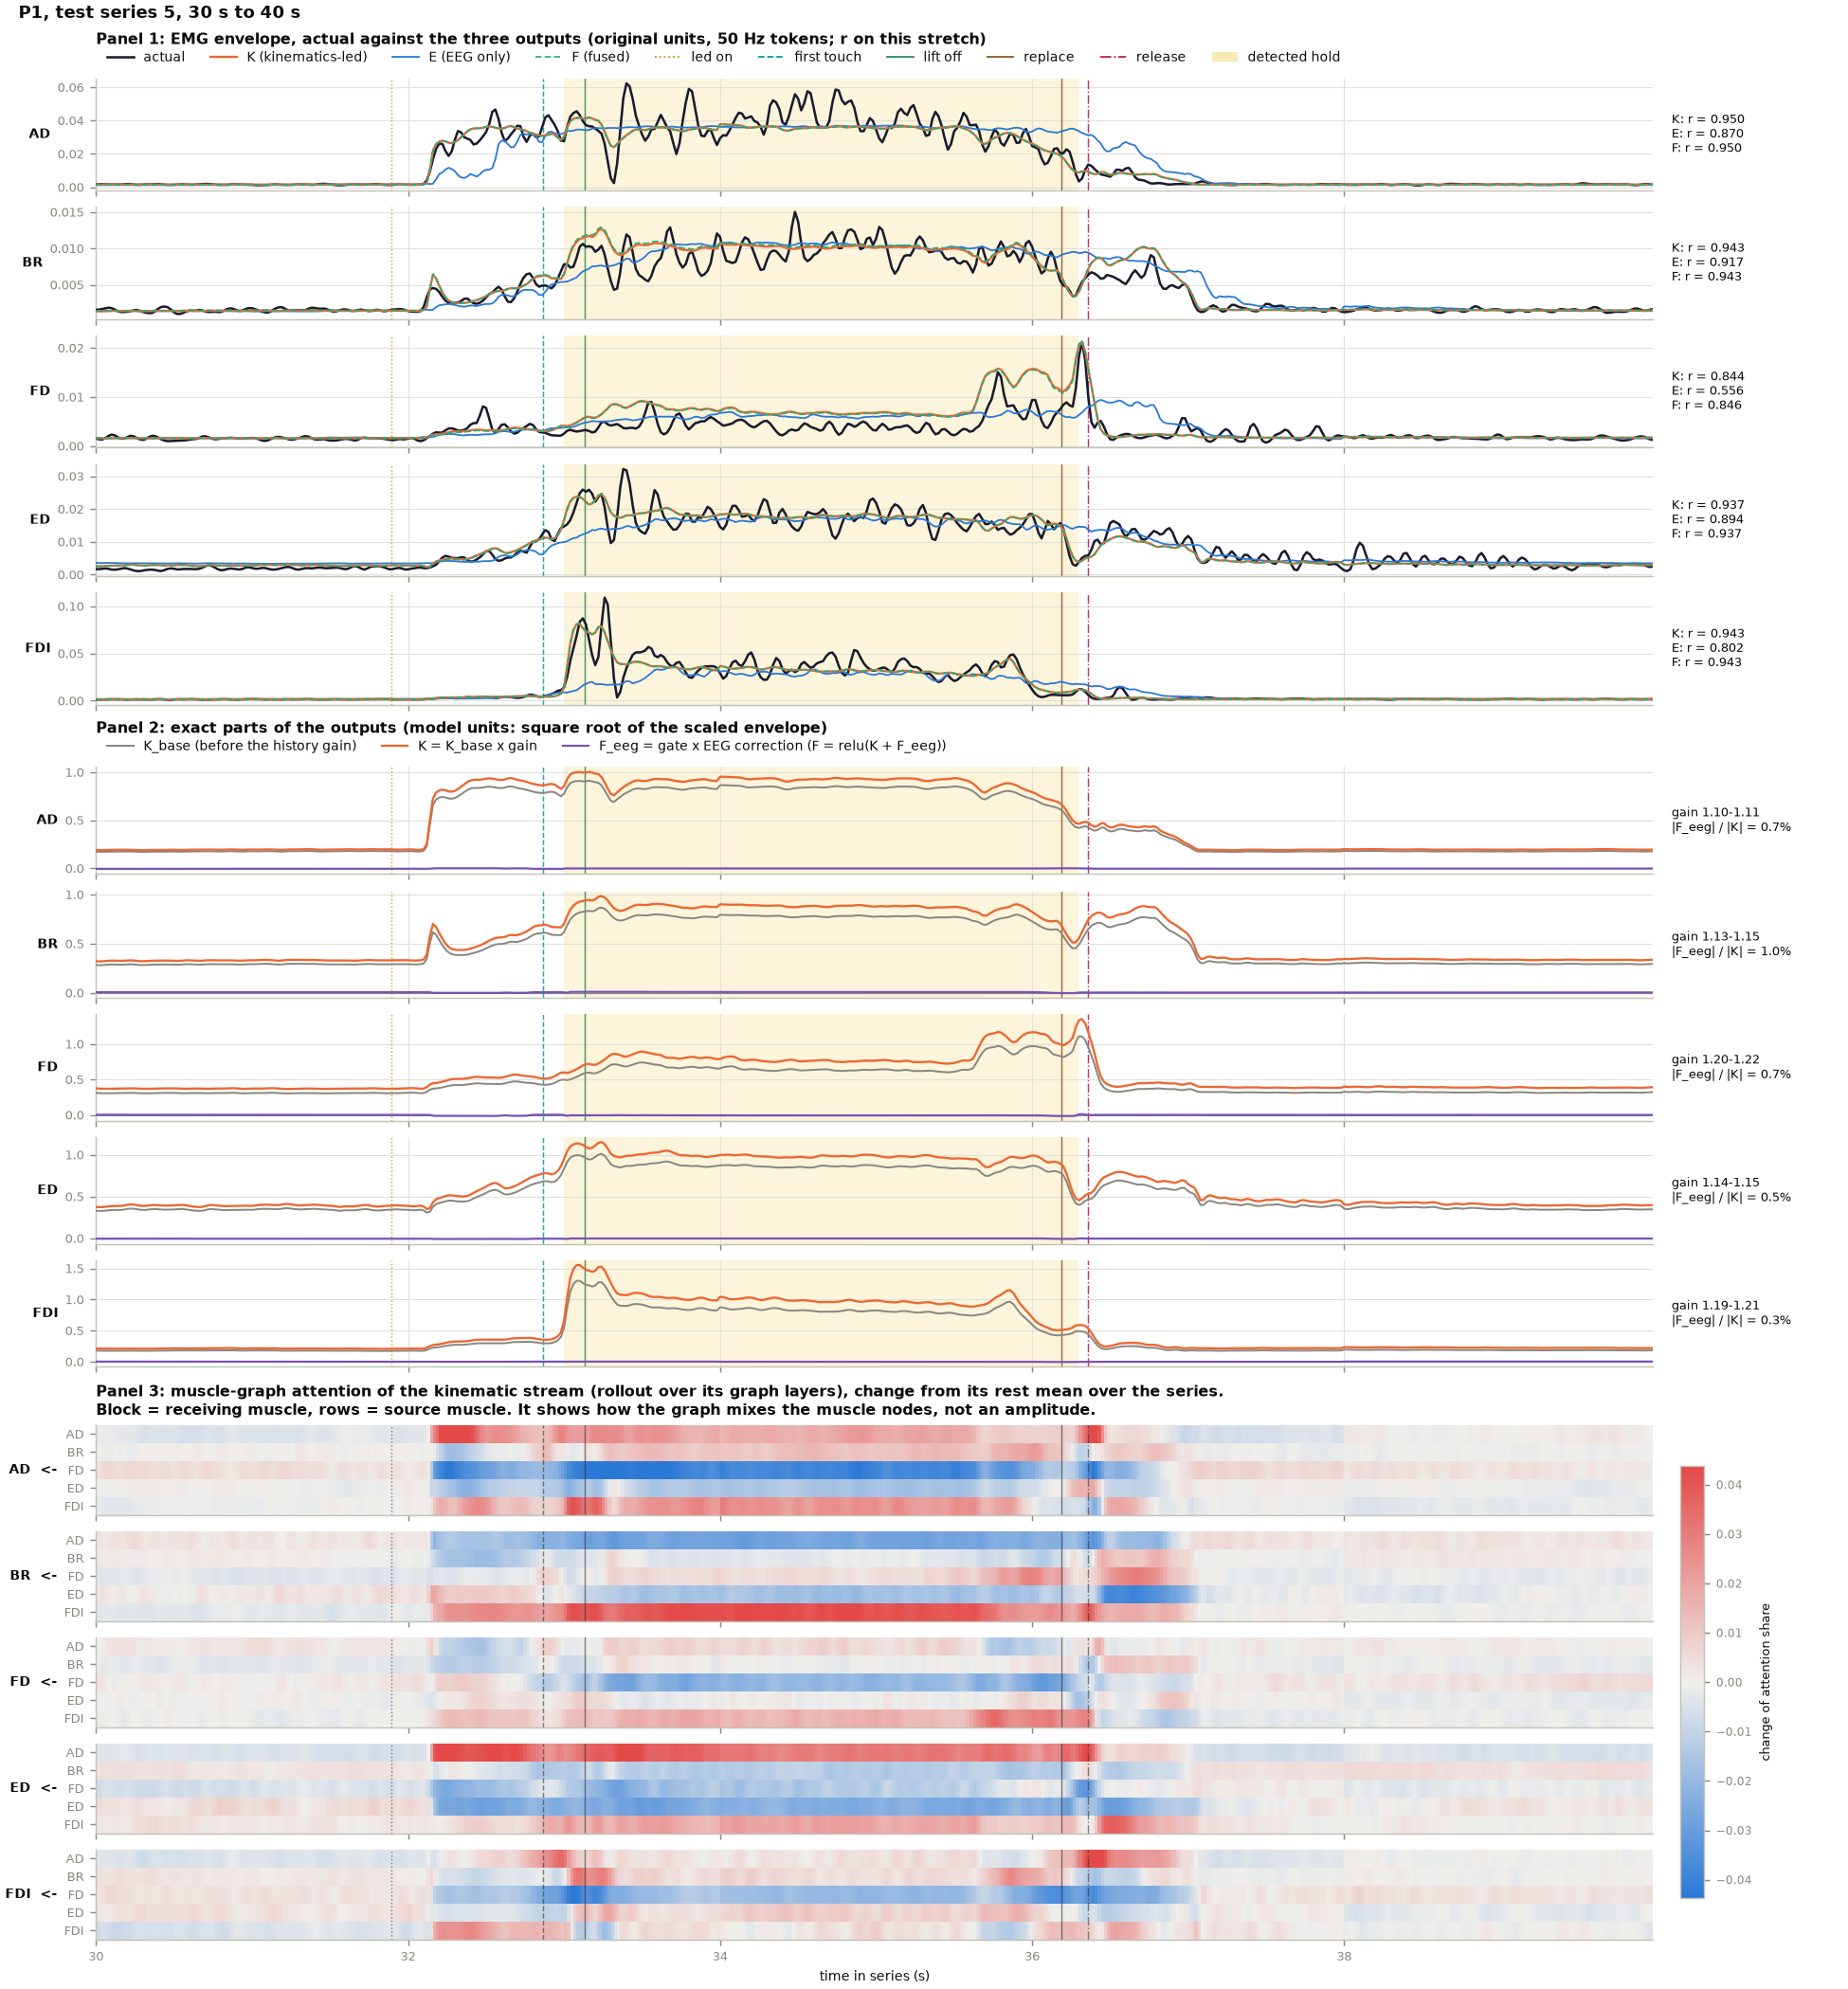
\includegraphics[height=66mm,width=\linewidth,keepaspectratio]{trip_P1_S05.png}}
    \column{0.52\linewidth}
    \begin{itemize}\scriptsize
      \item \textbf{Panel 1:} true envelope (black) against K (orange), E (blue) and F (dashed); task events as
            vertical lines, detected holds shaded; $r$ of each output on this stretch at the right.
      \item \textbf{Panel 2:} the exact parts of the output: K before the history gain, K after it, and the EEG
            correction $F_{eeg}$ (purple). $|F_{eeg}|/|K|$ is 0.3--2.8\% here.
      \item \textbf{Panel 3:} muscle-graph attention of the kinematic stream, change from its rest mean.
    \end{itemize}
    \begin{tcolorbox}[notebox,title={What the triptychs show}]
      K follows the envelope closely (here $r$ 0.85--0.92). E follows the task phases: it rises and falls with the
      holds but misses the level and the fast peaks, and in this stretch it can even be uncorrelated with a muscle
      (AD $r=-0.04$). The EEG correction in F is a flat line near zero.
    \end{tcolorbox}
  \end{columns}
\end{frame}

\begin{frame}{What the v2 triptych fixed compared with v1 (same stretch: P1, series 4, 30--40 s)}
  \begin{columns}[T]
    \column{0.24\linewidth}
    \FigRow{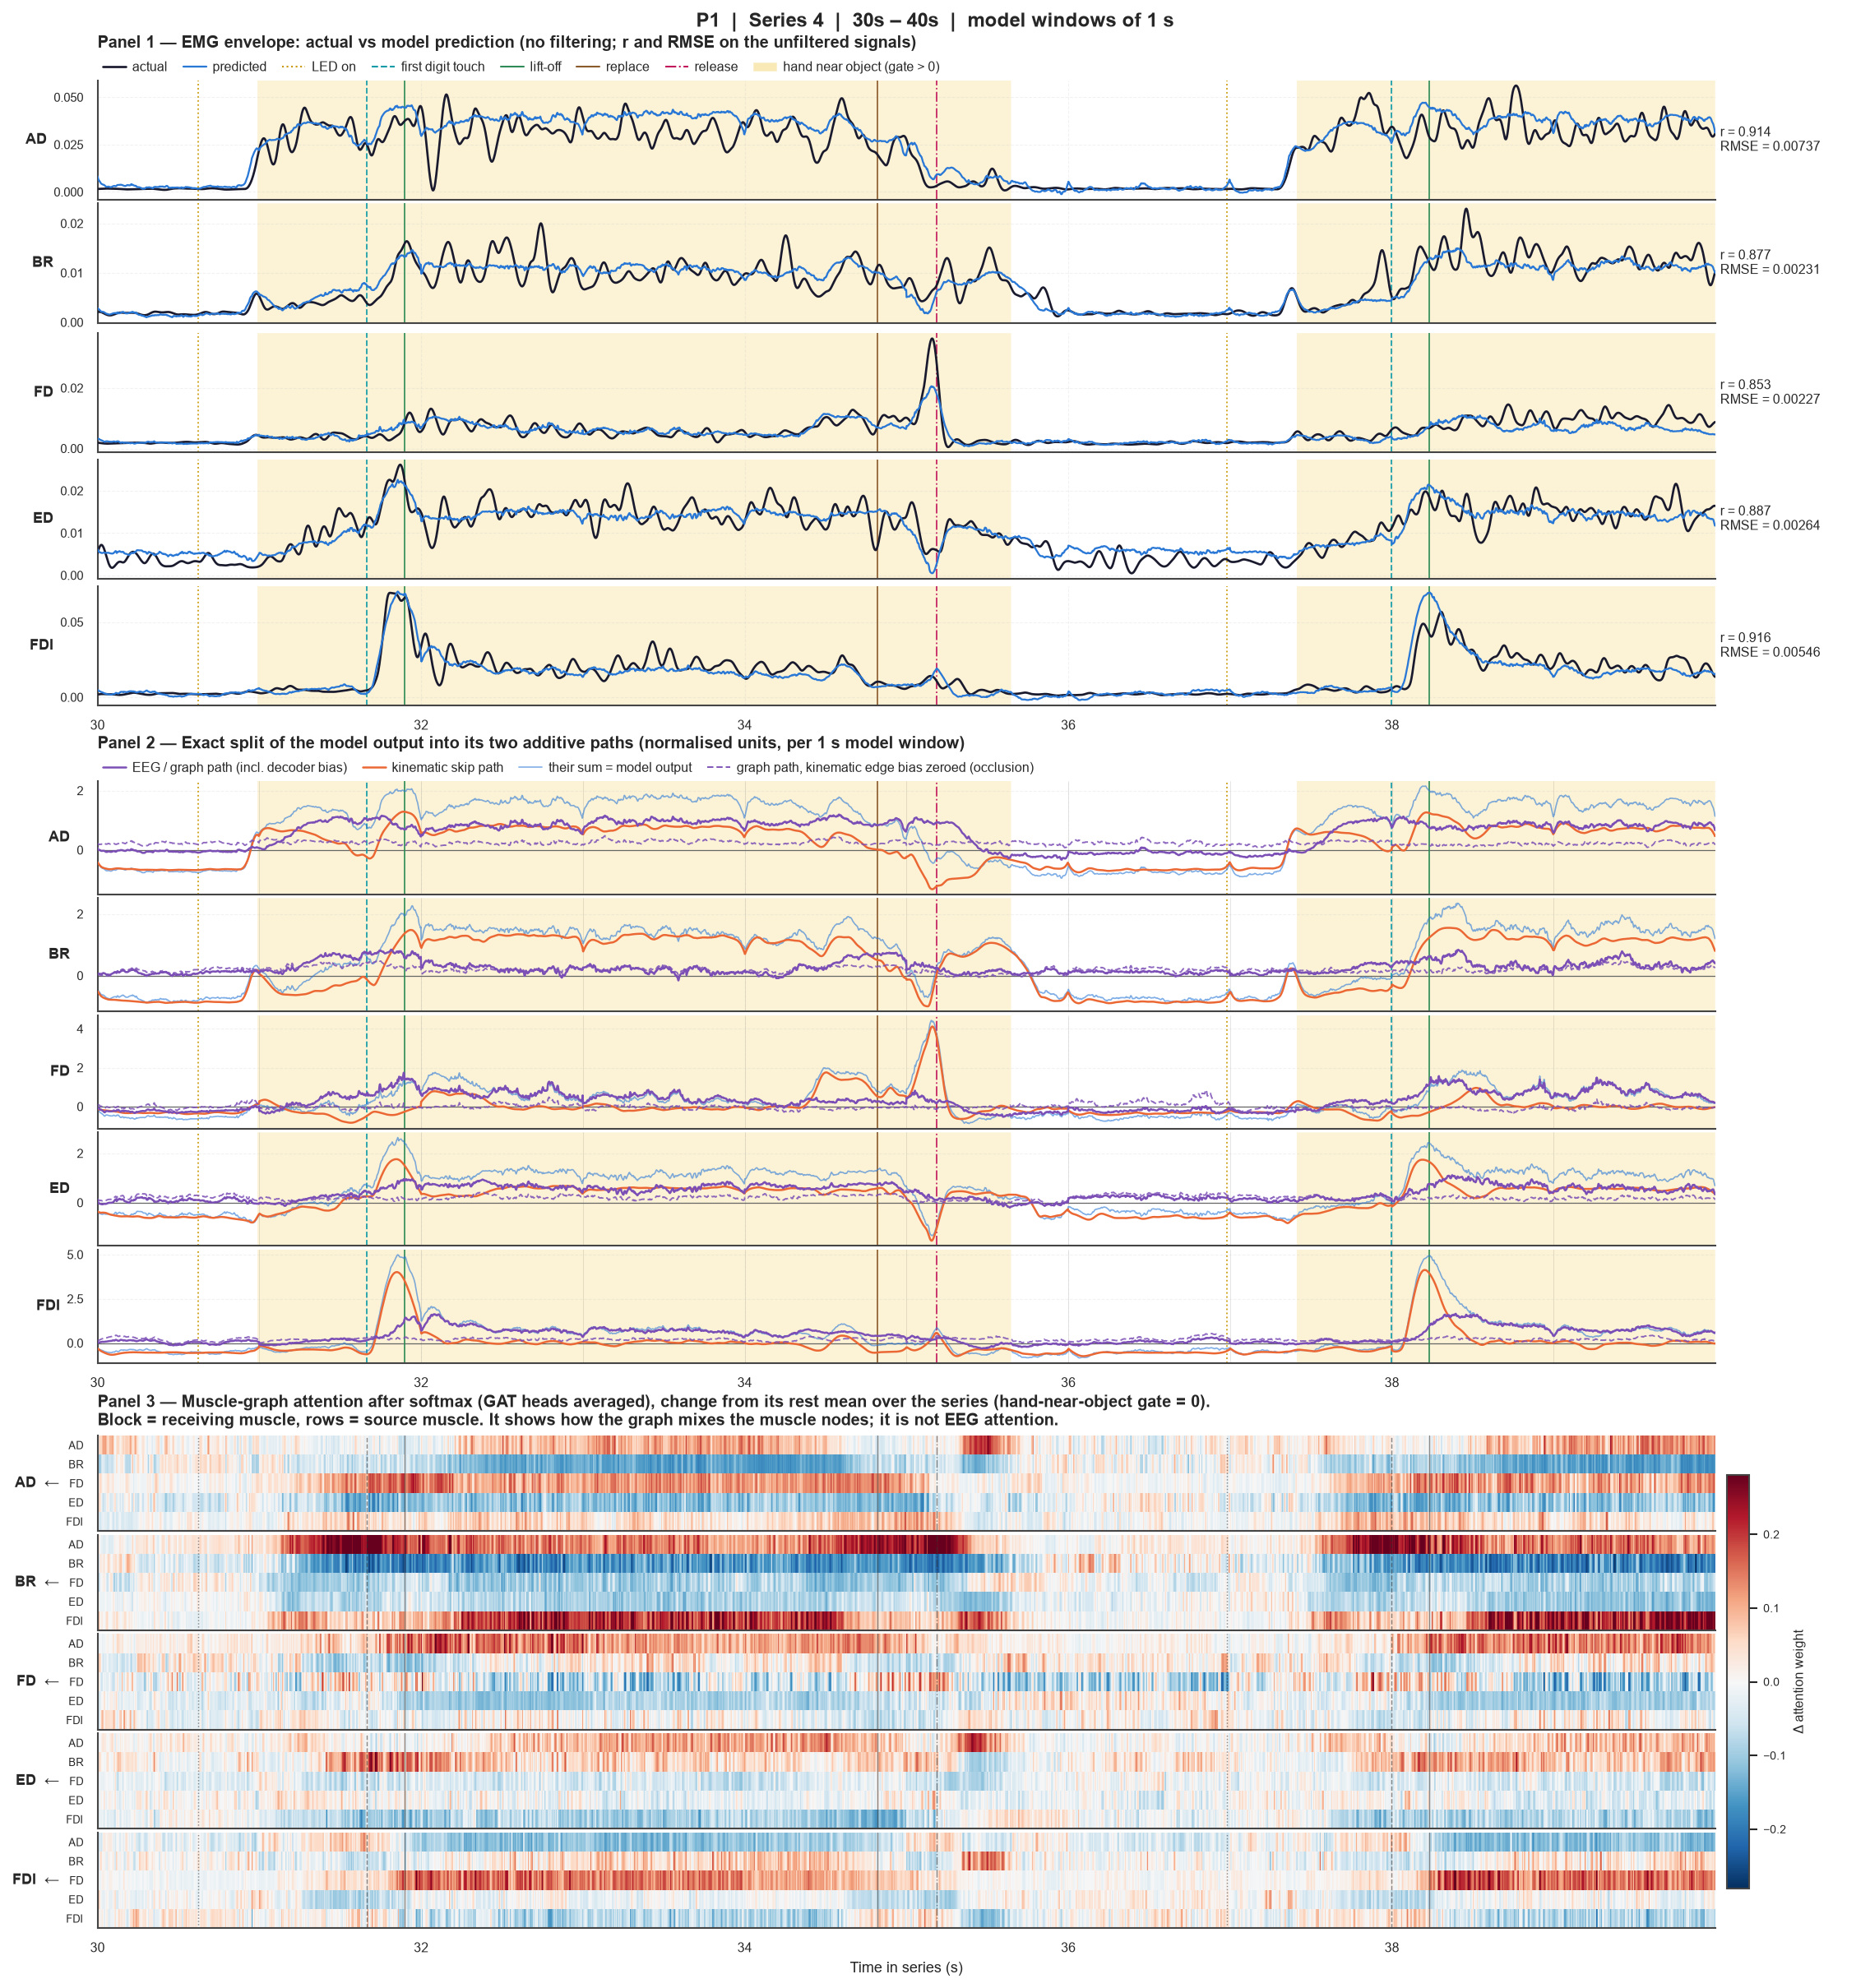
\includegraphics[height=34mm,width=\linewidth,keepaspectratio]{base_triptych_P1.png}}
    \FigCap{v1}
    \FigRow{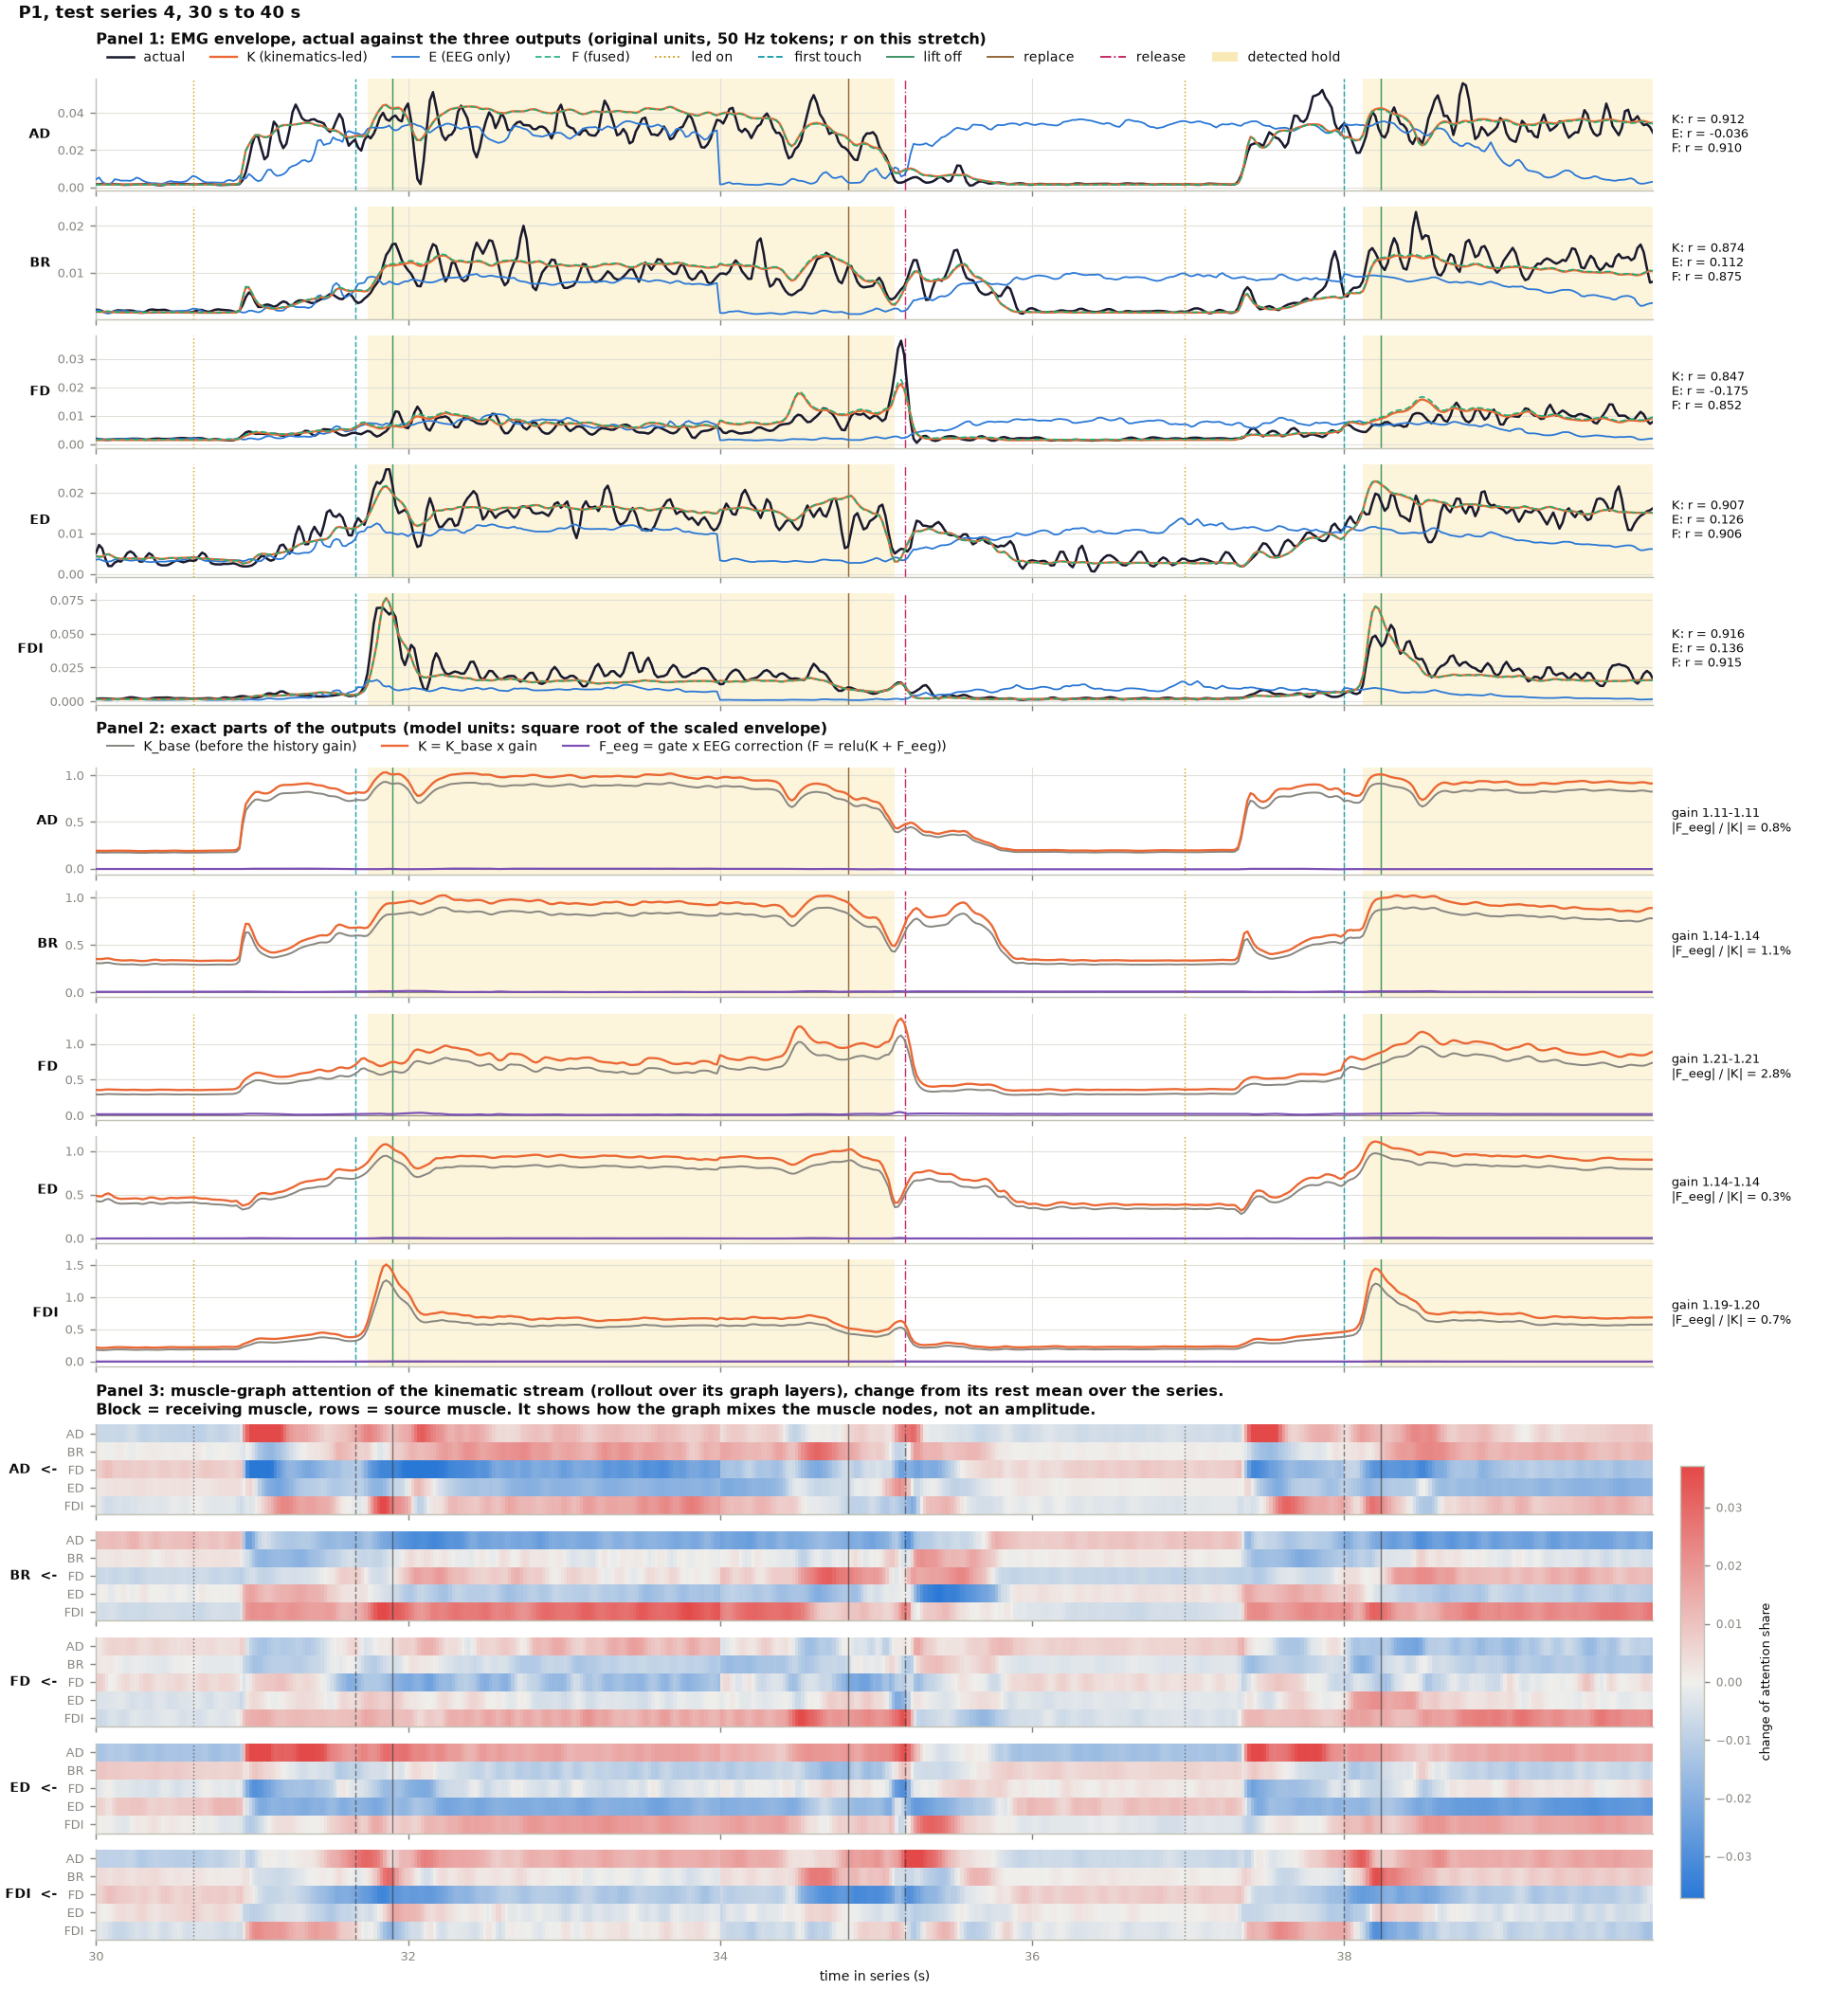
\includegraphics[height=34mm,width=\linewidth,keepaspectratio]{trip_P1_S04.png}}
    \FigCap{v2}
    \column{0.74\linewidth}
    \centering\scriptsize
    \renewcommand{\arraystretch}{1.15}
    \setlength{\tabcolsep}{3pt}
    \begin{tabular}{@{}>{\raggedright}p{10mm}>{\raggedright}p{30mm}>{\raggedright}p{35mm}>{\raggedright\arraybackslash}p{29mm}@{}}
      \toprule
      panel & v1 & v2 & what it fixes \\
      \midrule
      1 & one mixed prediction; shading = hand near object (force gate) & three outputs K, E, F with $r$ of each;
          shading = detected holds (the holds the \emph{lift} loss uses) & EEG-only accuracy (E) is visible
          directly, next to K \\
      2 & two paths of one output, per 1 s window, normalised units; the ``EEG/graph'' path is driven by the
          kinematic edge bias (dashed line) & exact parts in model units: $K_{base}$, $K=K_{base}\cdot g$ (history
          gain, its range printed), $F_{eeg}=\gamma\cdot$EEG correction with $|F_{eeg}|/|K|$ printed & every part
          has a single source, so the EEG share is a number (here 0.3--2.8\%) \\
      3 & one GAT layer, softmax attention, heads averaged; graph also guided by kinematics & attention rollout over
          the graph layers of the kinematic stream only & a pure, traceable kinematic graph; EEG attribution moves
          to the rollout analyses \\
      context & 1 s windows, 500 Hz & 8 s windows, 50 Hz tokens, stitched middle 4 s & long context; no window-edge
                 jumps \\
      \bottomrule
    \end{tabular}
  \end{columns}
\end{frame}

\begin{frame}{v2 test: the residual test, without the fusion module}
  \begin{columns}[T]
    \column{0.50\linewidth}
    \centering
    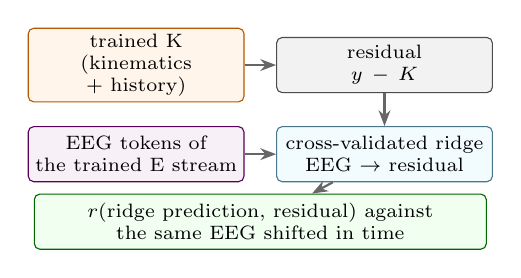
\begin{tikzpicture}[node distance=3mm and 4mm]
      \node[kin,text width=26mm] (k) {trained K\\(kinematics + history)};
      \node[res,text width=26mm,right=of k] (r) {residual\\$y-K$};
      \node[eeg,text width=26mm,below=of k] (e) {EEG tokens of\\the trained E stream};
      \node[blk,text width=26mm,right=of e] (ri) {cross-validated ridge\\EEG $\to$ residual};
      \node[good,text width=56mm,below=5mm of $(e)!0.5!(ri)$] (t) {$r$(ridge prediction, residual) against the same EEG shifted in time};
      \draw[arr] (k)--(r); \draw[arr] (e)--(ri); \draw[arr] (r)--(ri); \draw[arr] (ri)--(t);
    \end{tikzpicture}
    \column{0.46\linewidth}
    \begin{itemize}\scriptsize
      \item Question: does the fusion fail to use EEG, or is there nothing to use?
      \item EEG predicts K's error with $r\approx0.07$, significant in 10 of 12.
      \item Turned into accuracy, that is less than 0.5 VAF points.
      \item The fusion module had found the same small amount: $F\approx K$ is the correct answer, not a training
            failure.
    \end{itemize}
    \begin{tcolorbox}[notebox,title={E alone: the time-shift null}]
      E's $r$ 0.645 drops to near zero when the EEG blocks are shifted in time: significant in all 12. So E is not
      noise; the question is \emph{what} it knows.
    \end{tcolorbox}
  \end{columns}
\end{frame}

%% =============================================================
\section{v2 interpretability}
%% =============================================================

\begin{frame}{Interpretability: four attribution methods, two checks on the methods}
  \begin{columns}[T]
    \column{0.50\linewidth}
    \textbf{Methods} (one mixing rule per block makes them exact through all layers)
    \begin{itemize}\scriptsize
      \item \textbf{attention rollout}: multiplies attention matrices through the layers
      \item \textbf{attention flow}: max-flow through the attention graph, shown against a uniform-attention baseline
      \item \textbf{gradient-weighted rollout}: rollout weighted by the gradient of the output
      \item \textbf{gradient $\times$ input}: input features (kinematics, history, EEG bands)
    \end{itemize}
    \textbf{Checks on the methods}
    \begin{itemize}\scriptsize
      \item \textbf{deletion check}: delete the top-ranked inputs; a correct map changes the output more than random
            deletion
      \item \textbf{weight-shuffle check}: the same map on a model with shuffled weights must look different
    \end{itemize}
    \column{0.46\linewidth}
    \FigRow{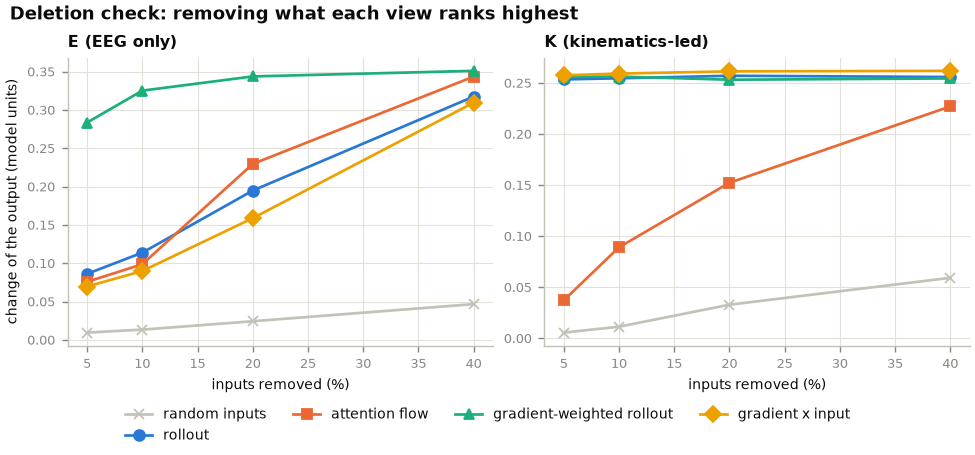
\includegraphics[width=\linewidth,height=30mm,keepaspectratio]{P1_deletion.png}}
    \FigCap{P1 deletion curves: a higher curve at small percentages = a better method.}
    \begin{itemize}\scriptsize
      \item For E, gradient-weighted rollout is best by far: output change 0.205 vs about 0.09 for the others and
            0.021 for random deletion; first in all 12.
      \item Attention flow saturates in this architecture (0.118 for K); it only means something against the uniform
            baseline.
      \item Plain rollout of K looks similar on the shuffled model ($r$ 0.47): its shape comes partly from the
            architecture.
    \end{itemize}
  \end{columns}
\end{frame}

\begin{frame}{Interpretability, P1: where in time do K and E look?}
  \begin{columns}[T]
    \column{0.49\linewidth}
    \FigRow{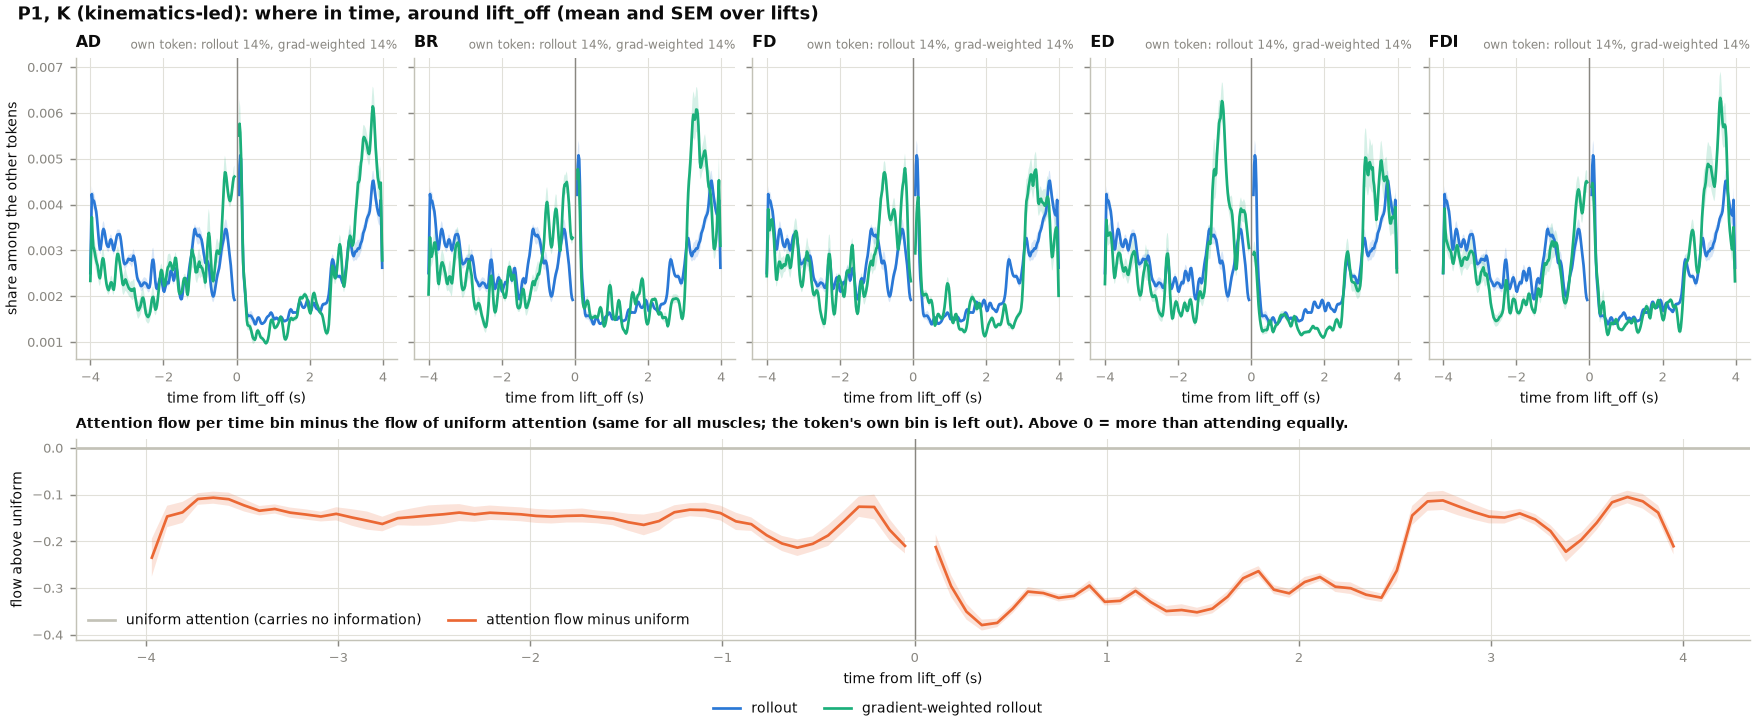
\includegraphics[width=\linewidth,height=34mm,keepaspectratio]{P1_time_K_lift_off.png}}
    \FigCap{K around lift-off: share of each time token (top), flow minus uniform flow (bottom).}
    \column{0.49\linewidth}
    \FigRow{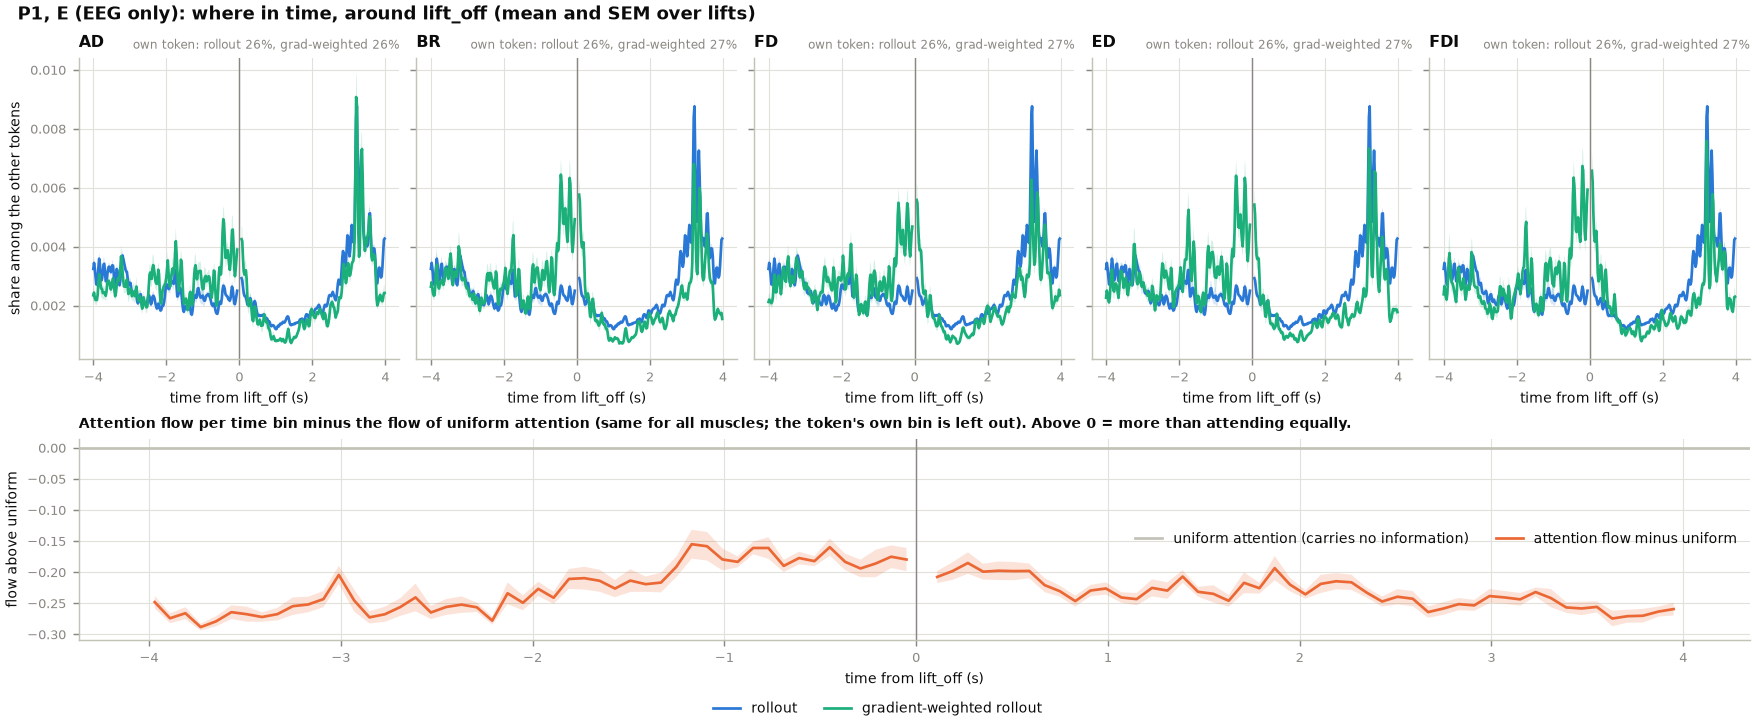
\includegraphics[width=\linewidth,height=34mm,keepaspectratio]{P1_time_E_lift_off.png}}
    \FigCap{E around lift-off. The moment itself carries 26\% of the share, more than for K.}
  \end{columns}
  \medskip
  \begin{itemize}\scriptsize
    \item K looks at the movement \emph{before} each event in every participant, and least at the 0--2.5 s after it.
    \item E's curve is flatter; in P2 it is almost flat with jumps only at the window edges (appendix).
  \end{itemize}
\end{frame}

\begin{frame}{Interpretability, P1: which electrodes, and against rest}
  \FigRow{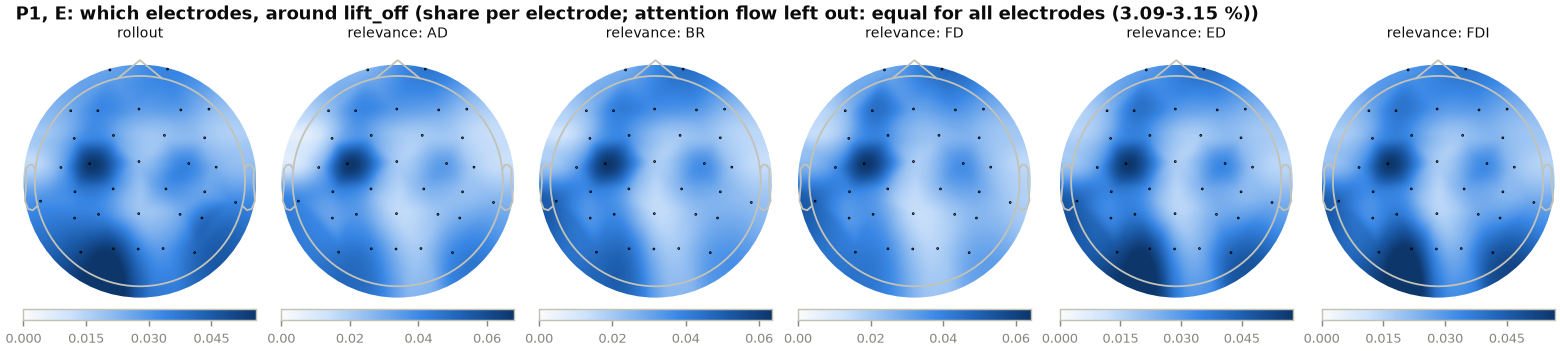
\includegraphics[width=\textwidth,height=23mm,keepaspectratio]{P1_scalp_E_lift_off.png}}
  \FigCap{E: electrode share per muscle, rollout and gradient-weighted rollout. Main focus: left central (C3).}
  \vspace{2mm}
  \FigRow{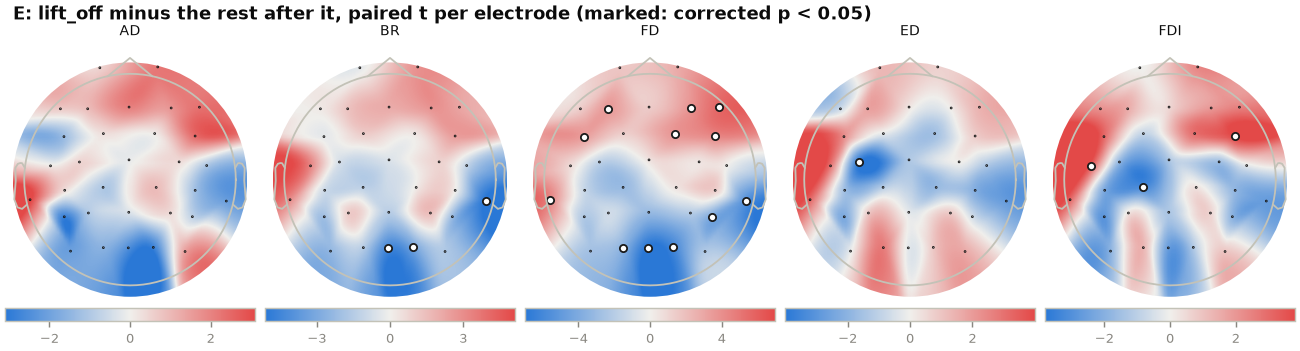
\includegraphics[width=\textwidth,height=23mm,keepaspectratio]{P1_rest_contrast_lift_off.png}}
  \FigCap{E: electrode share at lift-off minus the rest that follows, paired $t$; circles: corrected $p<0.05$.}
  \begin{itemize}\scriptsize
    \item P1 has a clear left central focus over the hand area. In P2 it is weaker and the edge electrodes weigh more
          (appendix): single maps are noisy, which is why the group analysis matters.
  \end{itemize}
\end{frame}

\begin{frame}{Interpretability, P1: input features and the muscle graph}
  \begin{columns}[T]
    \column{0.46\linewidth}
    \FigRow{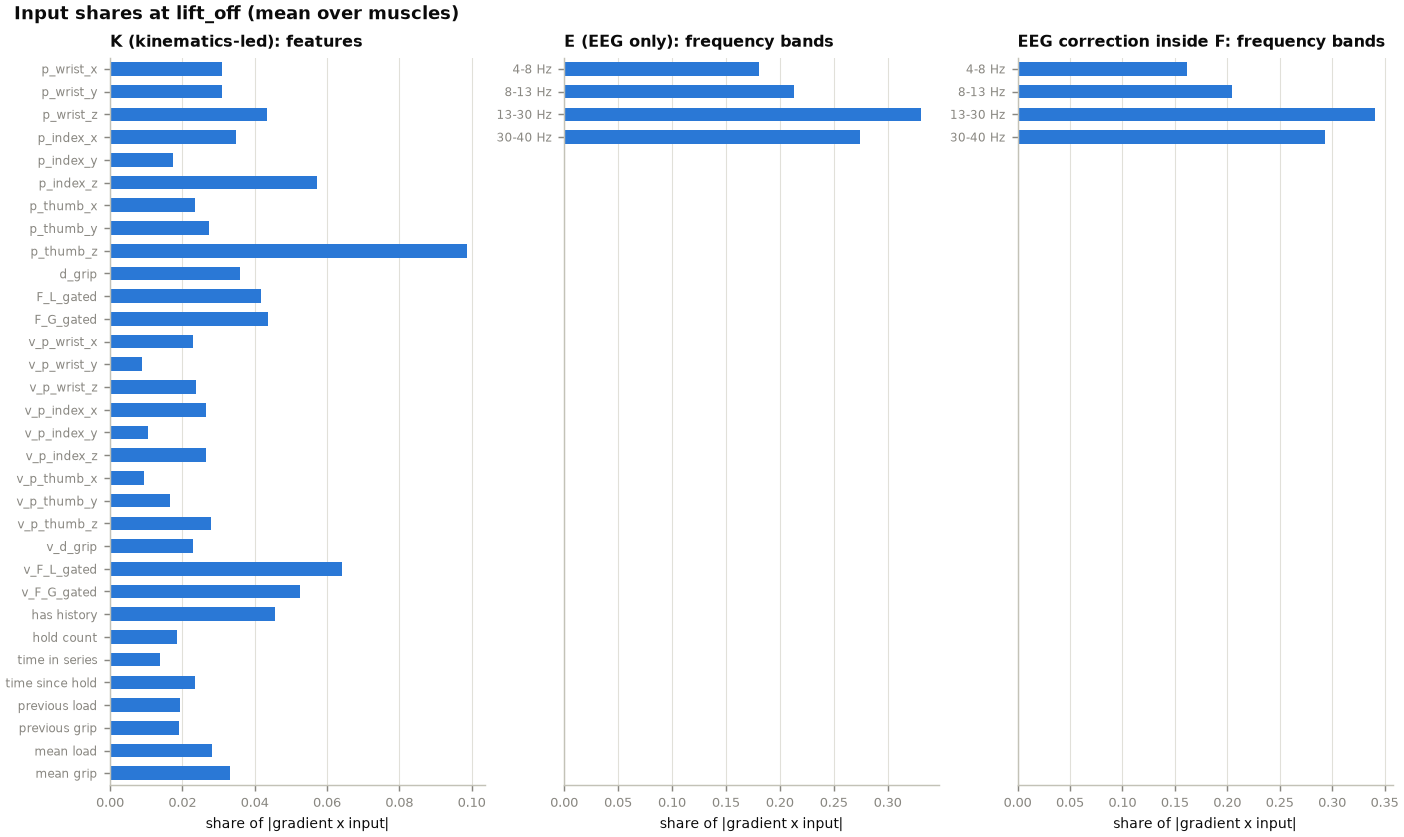
\includegraphics[width=\linewidth,height=50mm,keepaspectratio]{P1_inputs_lift_off.png}}
    \FigCap{Gradient $\times$ input: kinematic and history features in K, EEG bands in E and in F's EEG correction.}
    \column{0.50\linewidth}
    \FigRow{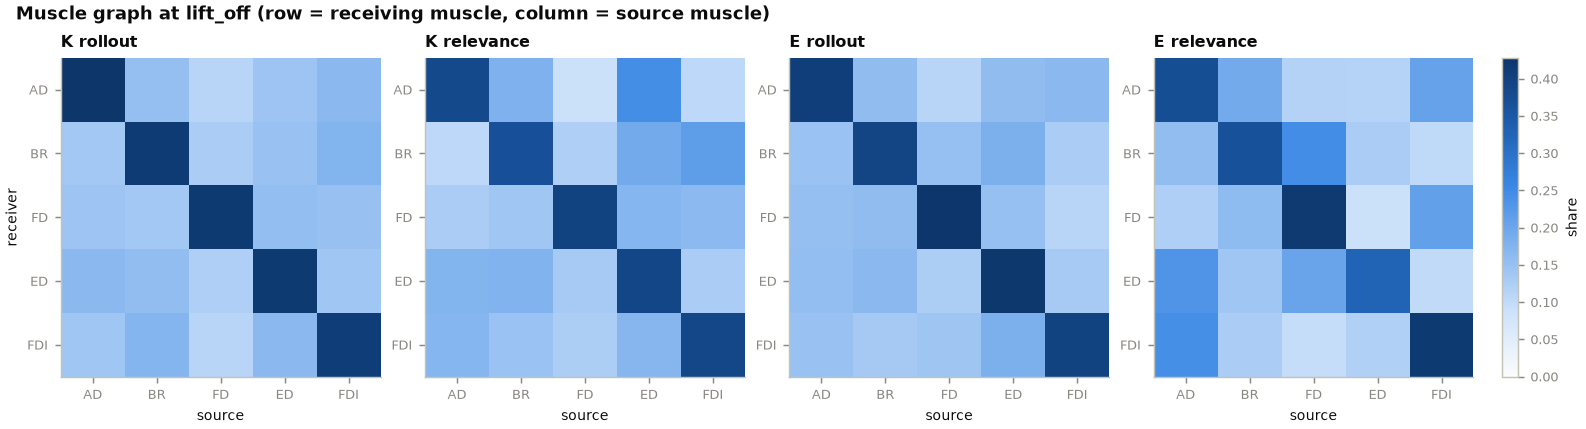
\includegraphics[width=\linewidth,height=20mm,keepaspectratio]{P1_muscle_graph_lift_off.png}}
    \FigCap{Muscle graph at lift-off for K and E, rollout and gradient-weighted rollout.}
    \vspace{2mm}
    \FigRow{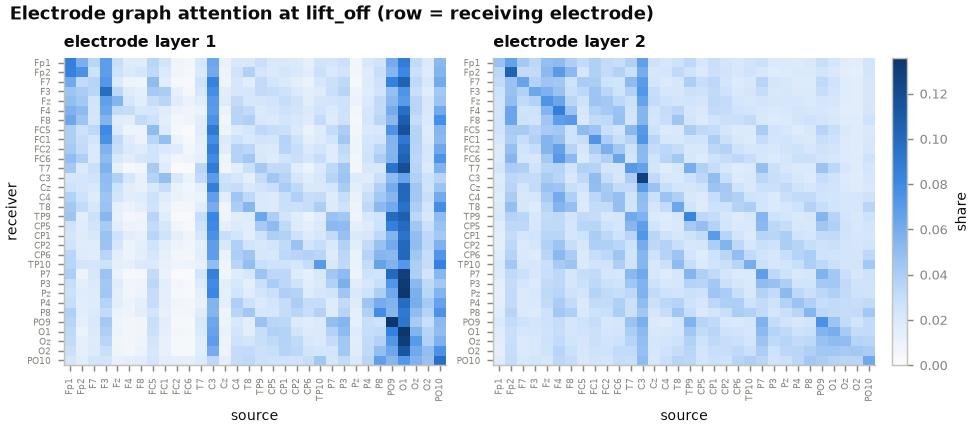
\includegraphics[width=\linewidth,height=24mm,keepaspectratio]{P1_electrode_layers_lift_off.png}}
    \FigCap{Attention of the two electrode-graph layers at lift-off; hubs in layer 1: C3 and O1.}
  \end{columns}
\end{frame}

\begin{frame}{Interpretability across the 12 participants: electrode maps}
  \FigRow{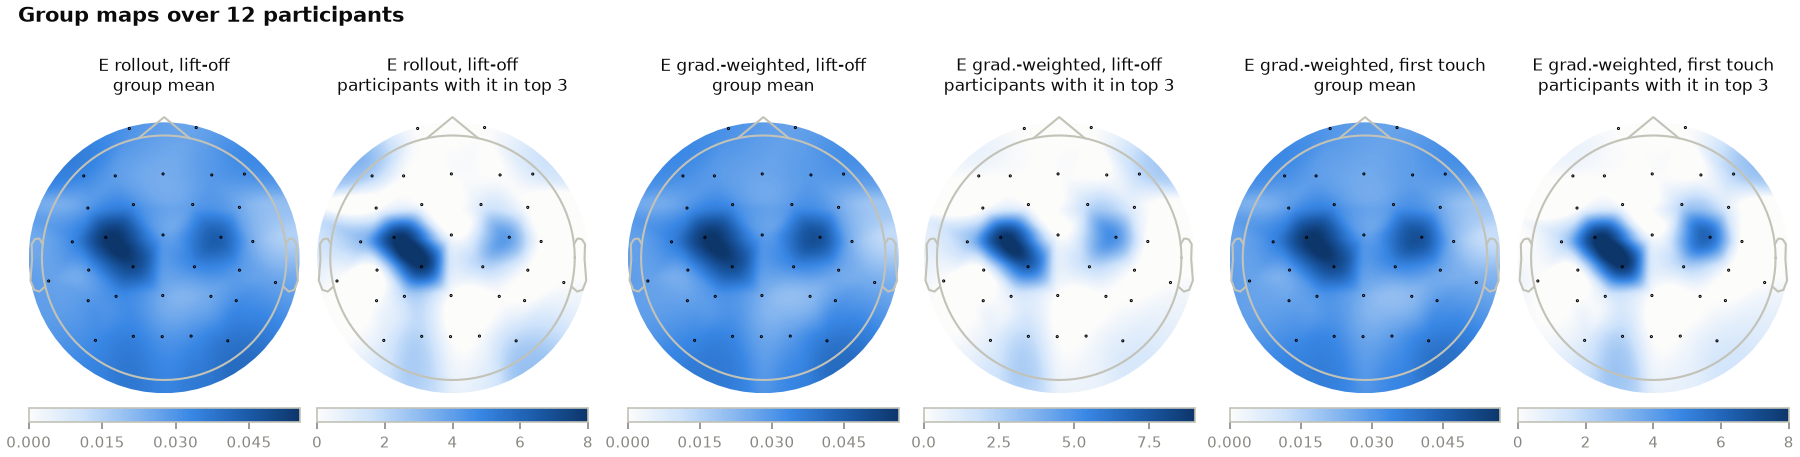
\includegraphics[width=\textwidth,height=27mm,keepaspectratio]{cons_scalp.png}}
  \FigCap{Group map of E (mean of 12) and the number of participants with each electrode in their top 3.}
  \begin{columns}[T]
    \column{0.55\linewidth}
    \FigRow{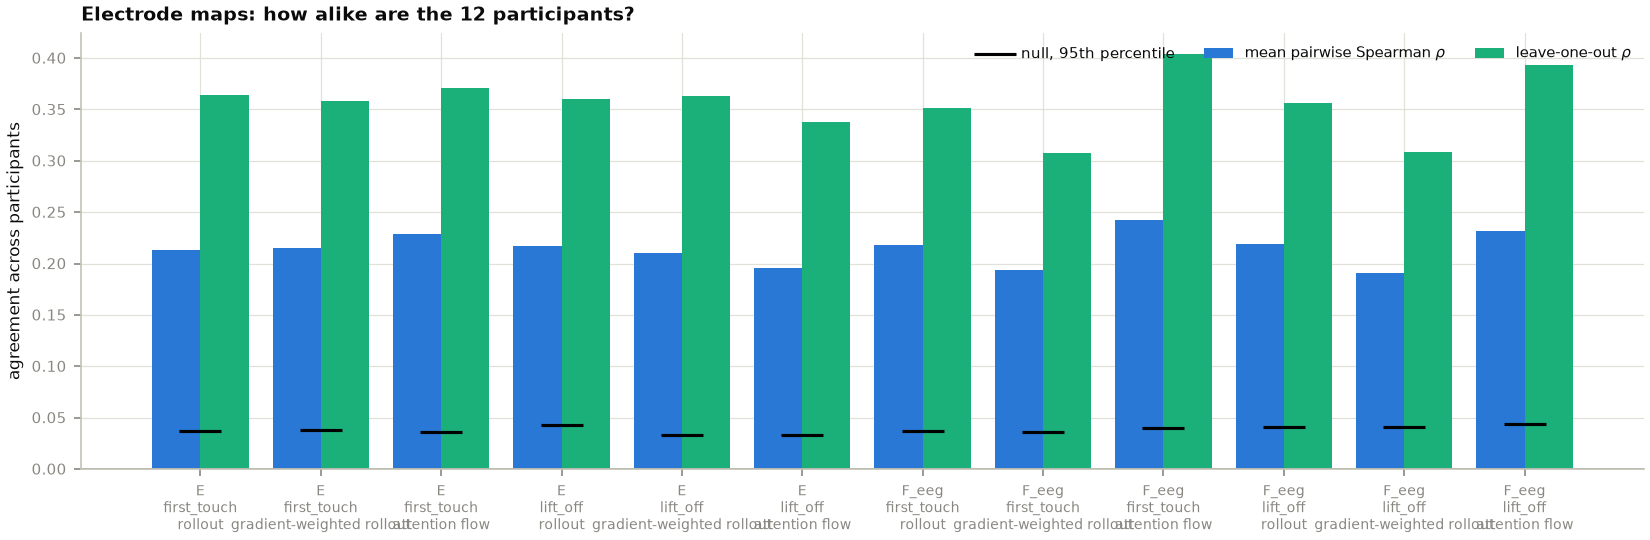
\includegraphics[width=\linewidth,height=26mm,keepaspectratio]{cons_electrodes.png}}
    \FigCap{Pairwise $\rho$ (blue) and leave-one-out $\rho$ (green) against the 95th percentile of the null.}
    \column{0.41\linewidth}
    \begin{itemize}\scriptsize
      \item One participant's map is noisy: pairwise $\rho$ 0.20--0.24.
      \item The group map is reproducible: leave-one-out $\rho$ 0.31--0.40, split-half about 0.7, above the null.
      \item Two significant foci: \textbf{C3} and \textbf{CP1}.
    \end{itemize}
  \end{columns}
\end{frame}

\begin{frame}{Interpretability across the 12 participants: time and bands}
  \begin{columns}[T]
    \column{0.58\linewidth}
    \FigRow{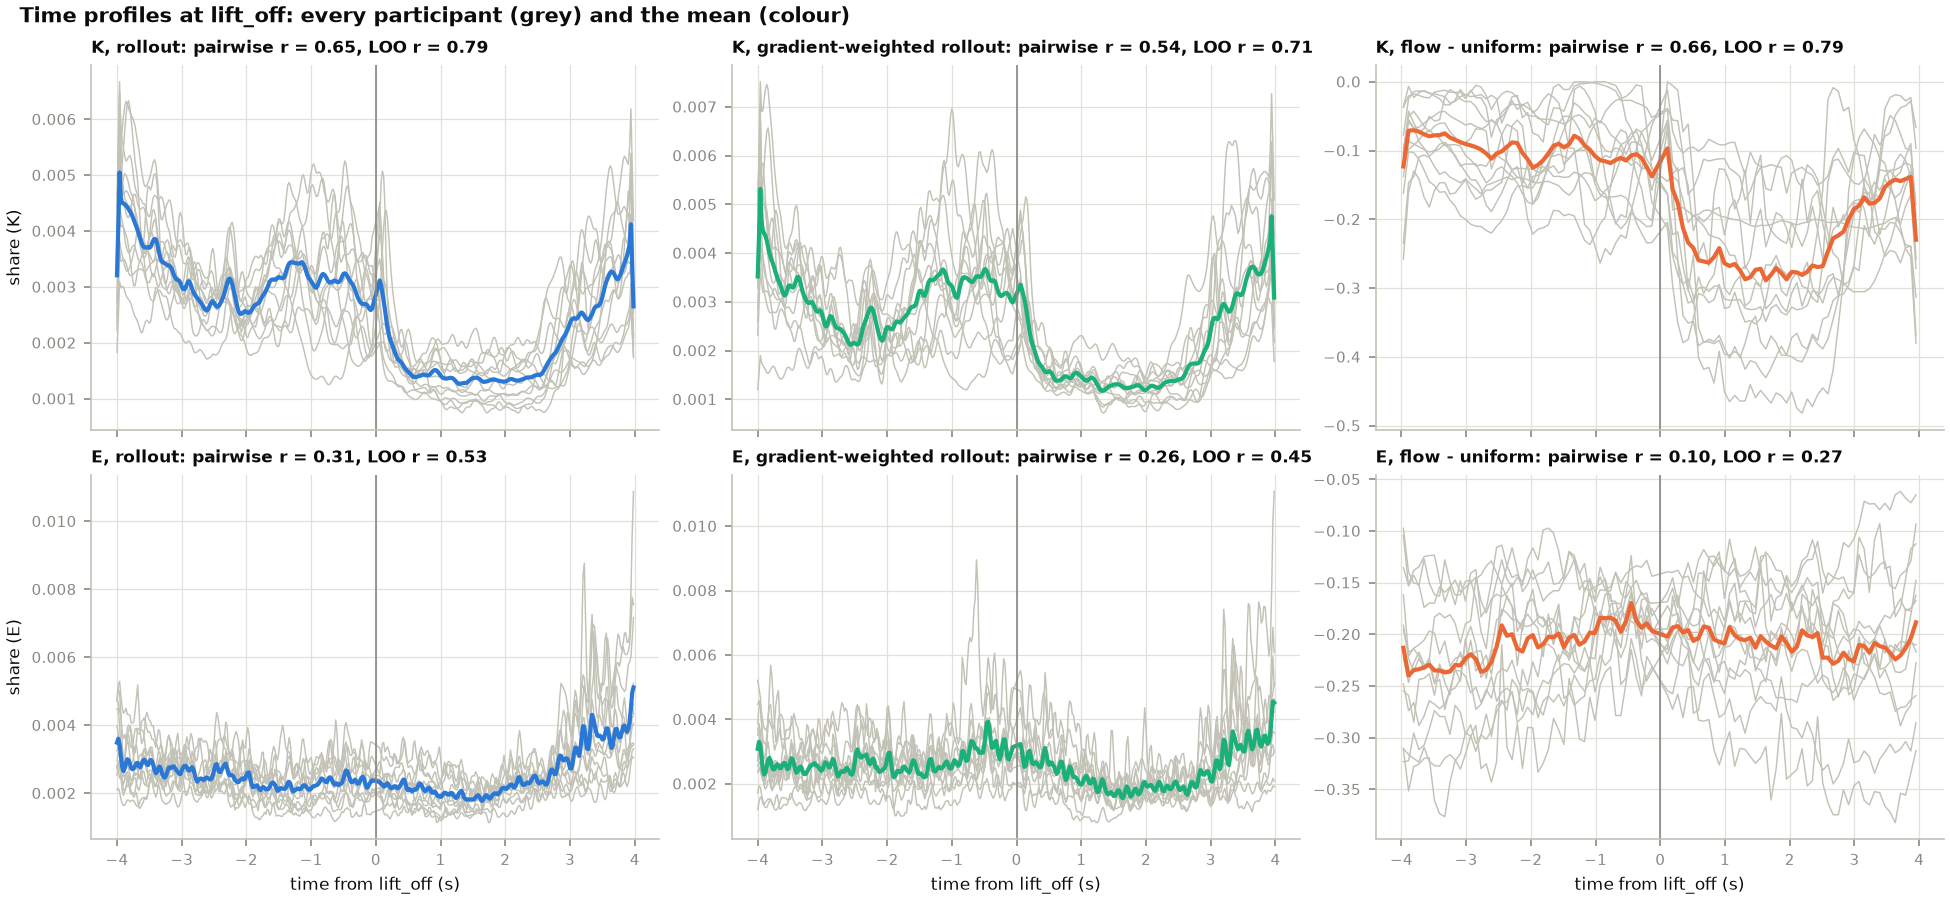
\includegraphics[width=\linewidth,height=33mm,keepaspectratio]{cons_time.png}}
    \FigCap{Time curves around lift-off, every participant (grey) and the mean. Top: K. Bottom: E.}
    \FigRow{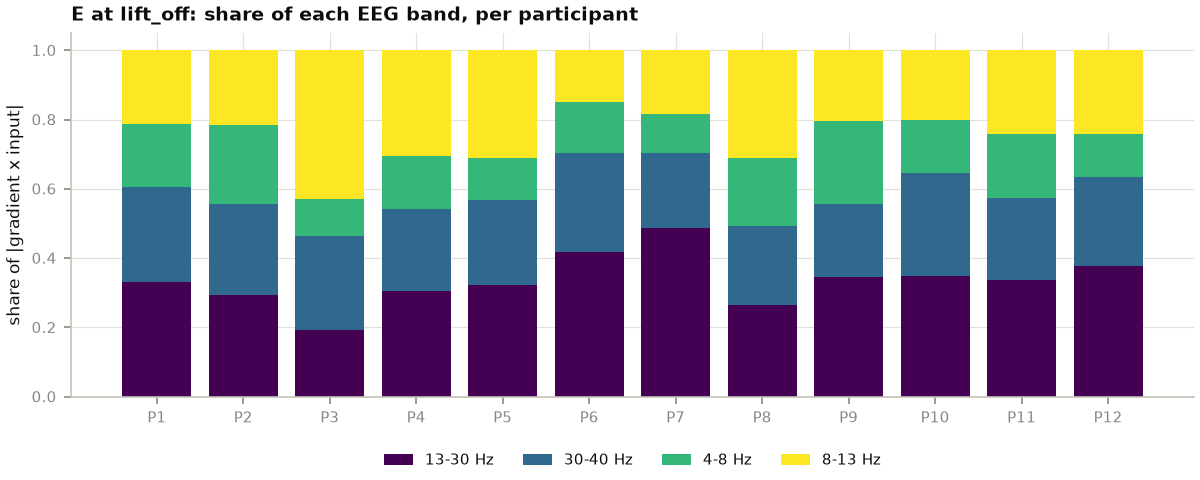
\includegraphics[width=\linewidth,height=22mm,keepaspectratio]{cons_bands.png}}
    \FigCap{Share of each EEG band in E at lift-off, per participant.}
    \column{0.38\linewidth}
    \begin{itemize}\scriptsize
      \item E prefers the \textbf{beta} band.
      \item Its attention peaks about 0.5--0.8 s \emph{before} the events.
      \item Both agree with the ERD literature.
      \item But E predicts the shoulder (AD) better than the finger muscles and has no muscle-specific map, which
            does not agree with the corticomuscular-coherence literature.
    \end{itemize}
    \begin{tcolorbox}[askbox,title={Doubt this raised}]
      \scriptsize A motor-cortex-like map, but the same map for every muscle. Is E reading motor commands or the
      phase of the task?
    \end{tcolorbox}
  \end{columns}
\end{frame}

%% =============================================================
\section{Controls: is it the task clock?}
%% =============================================================

\begin{frame}{Three controls, each testing one alternative explanation of E}
  \begin{columns}[T]
    \column{0.31\linewidth}
    \begin{tcolorbox}[stagebox,title={A. Task timing}]
      \scriptsize A linear ridge model that sees no body or brain signal, only the times of the 8 task events of each
      lift. If it beats E, E's accuracy can be explained by the task clock.
    \end{tcolorbox}
    \column{0.31\linewidth}
    \begin{tcolorbox}[stagebox,title={B. Reference maps}]
      \scriptsize Compare E's electrode map with the classic maps of the same data: beta/alpha ERD and beta
      corticomuscular coherence (CMC). Agreement points to sensorimotor cortex.
    \end{tcolorbox}
    \column{0.31\linewidth}
    \begin{tcolorbox}[stagebox,title={C. Prediction horizon}]
      \scriptsize A causal v2 predicting EMG 0, 200, 500 and 1000 ms ahead (48 models). Motor commands precede
      movement, so EEG should help more as the horizon grows.
    \end{tcolorbox}
  \end{columns}
  \medskip
  \begin{tcolorbox}[notebox,title={Why these three}]
    \scriptsize E reaches $r$ 0.645 alone but adds nothing to K. Three explanations are possible: (A) E only knows
    \emph{when} the task happens; (B) E reads artifacts rather than sensorimotor cortex; (C) EEG helps only ahead of
    the movement, which an offline model at horizon 0 cannot show. Each control tests one of them on all 12
    participants, with the participant as the unit of every group test.
  \end{tcolorbox}
\end{frame}

\begin{frame}{Control A, the features: what a ``timing feature'' is}
  \begin{columns}[T]
    \column{0.46\linewidth}
    \FigRow{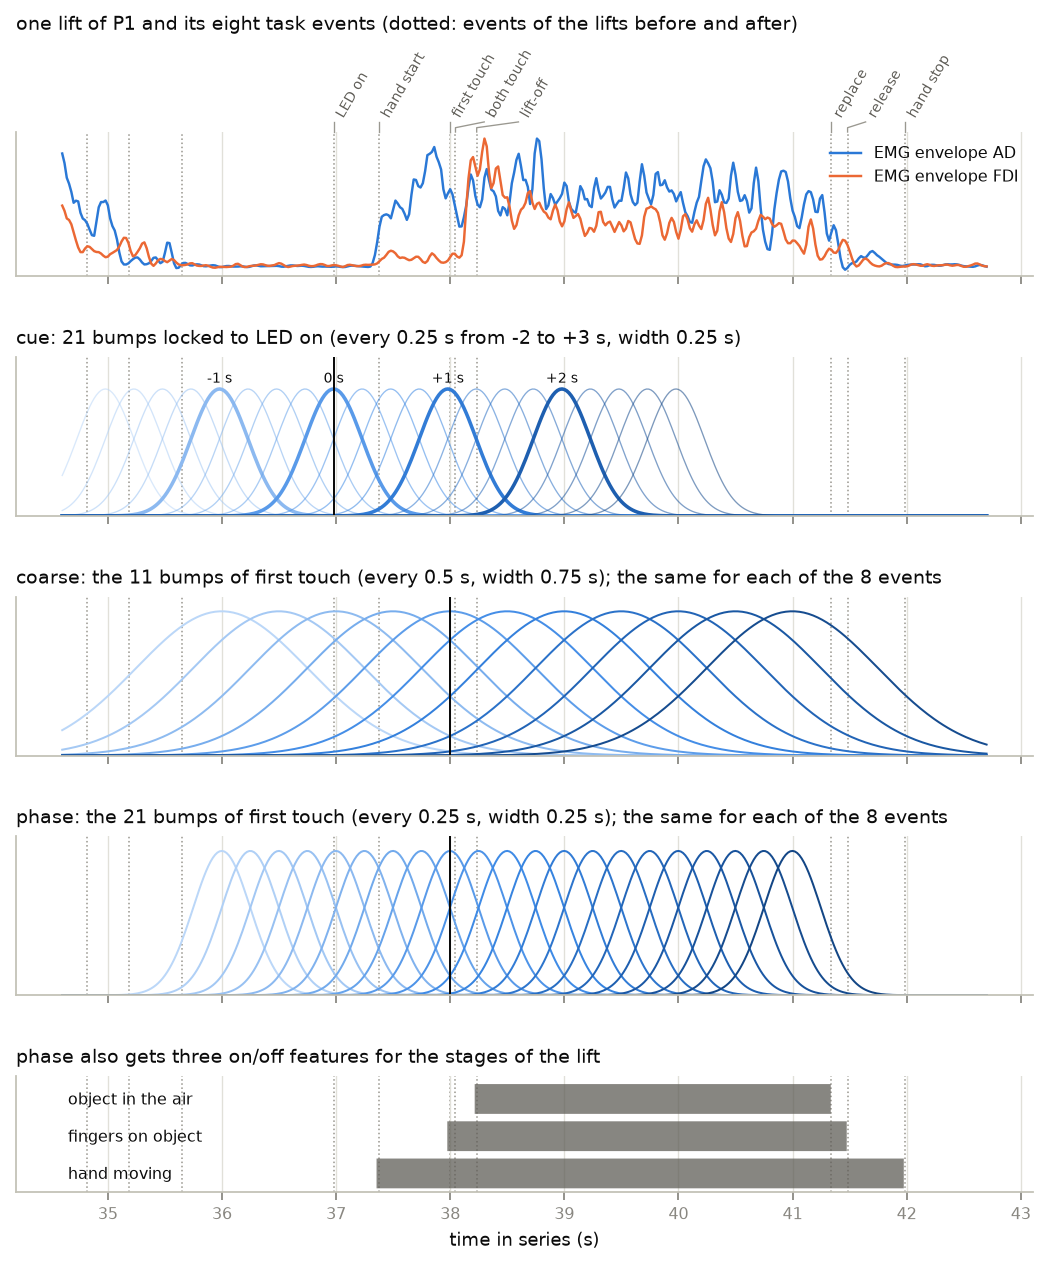
\includegraphics[height=76mm,width=\linewidth,keepaspectratio]{ctrl_features_bumps.png}}
    \column{0.52\linewidth}
    \textbf{Rows of the figure (one real lift of P1)}
    \begin{enumerate}\scriptsize\setlength{\itemsep}{0pt}
      \item \textbf{One lift and its 8 events}: LED on, hand start, first touch, both touch, lift-off, replace,
            release, hand stop (dotted: events of the lifts before and after). AD rises just after hand start; FDI
            peaks at touch. These peaks come at a nearly fixed distance from the events.
      \item \textbf{cue}: 21 Gaussian bumps locked to LED on, every 0.25 s from $-2$ to $+3$ s, width 0.25 s; four
            are drawn bold ($-1$, 0, $+1$, $+2$ s). Together they cover 5 s, so a ridge can build any smooth time
            pattern that repeats relative to the LED.
      \item \textbf{coarse}: 11 wide bumps per event (every 0.5 s, width 0.75 s), shown for first touch; only slow
            changes.
      \item \textbf{phase}: 21 narrow bumps per event (every 0.25 s); can follow a short peak like FDI at touch.
      \item \textbf{phase stages}: three on/off features (hand moving, fingers on object, object in the air) that give
            a constant level during long holds, beyond the 3 s reach of the bumps.
    \end{enumerate}
    \begin{tcolorbox}[notebox,title={The model}]
      \scriptsize Ridge per muscle on $u=\sqrt{y/s_c}$ (as v2). Event times include the future: a \emph{ceiling}.
    \end{tcolorbox}
  \end{columns}
\end{frame}

\begin{frame}{Control A, the features: the full input matrix of each version}
  \begin{columns}[T]
    \column{0.46\linewidth}
    \FigRow{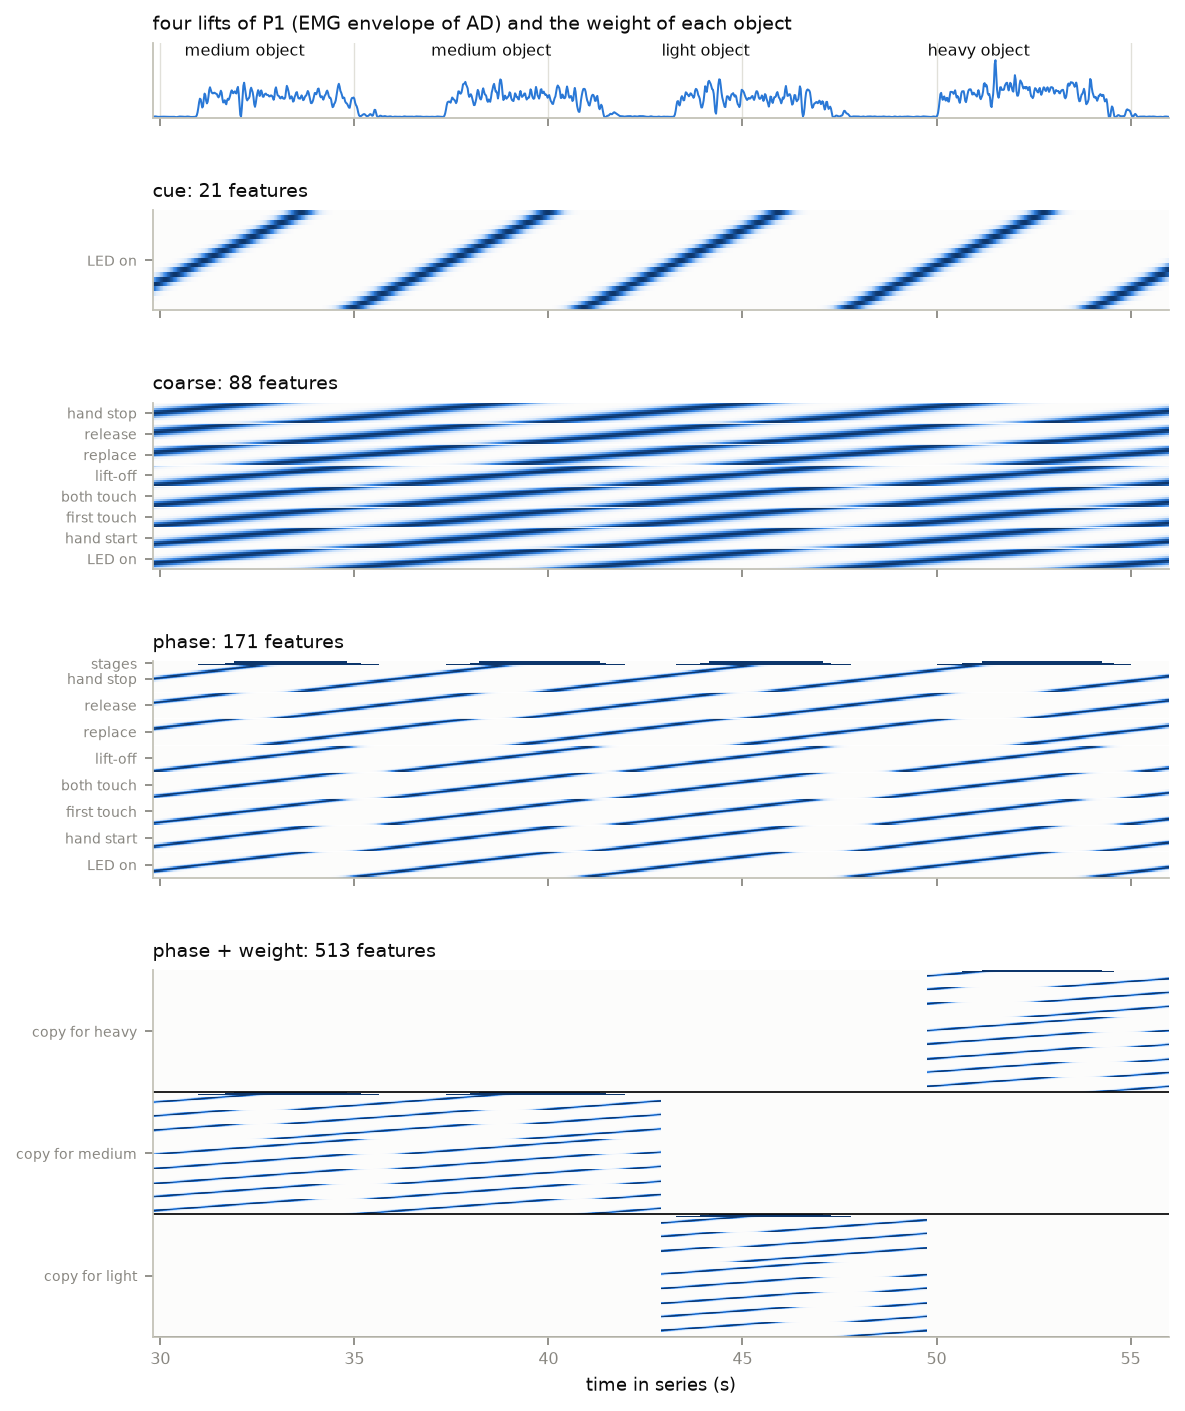
\includegraphics[height=76mm,width=\linewidth,keepaspectratio]{ctrl_features_matrix.png}}
    \column{0.52\linewidth}
    \textbf{Rows of the figure (four consecutive lifts of P1)}
    \begin{enumerate}\scriptsize
      \item \textbf{Top}: AD envelope and the weight of each object (medium, medium, light, heavy).
      \item \textbf{cue (21 features)}: one band of bumps per lift. Each bump peaks a little later than the one before,
            so together they draw a diagonal line.
      \item \textbf{coarse (88 = 8 events $\times$ 11)}: one diagonal per event, stacked in the time order of the lift.
      \item \textbf{phase (171 = 8 $\times$ 21 + 3 stages)}: the same with narrow bumps; the 3 stage rows on top.
      \item \textbf{phase + weight (513 = 3 $\times$ 171)}: three copies of phase, one per weight; in each lift only
            the copy of that object's weight is on, so a separate pattern per weight can be learned (for example
            more activity when holding the heavy object).
    \end{enumerate}
    \begin{tcolorbox}[notebox,title={How to read the results that follow}]
      \scriptsize From cue to phase + weight, each version knows more about timing. E never receives the weight, so
      phase + weight is only an upper reference; the fair comparison for E is \textbf{phase}.
    \end{tcolorbox}
  \end{columns}
\end{frame}

\begin{frame}{Control A: a model with no brain beats the EEG-only output}
  \begin{columns}[T]
    \column{0.52\linewidth}
    \FigRow{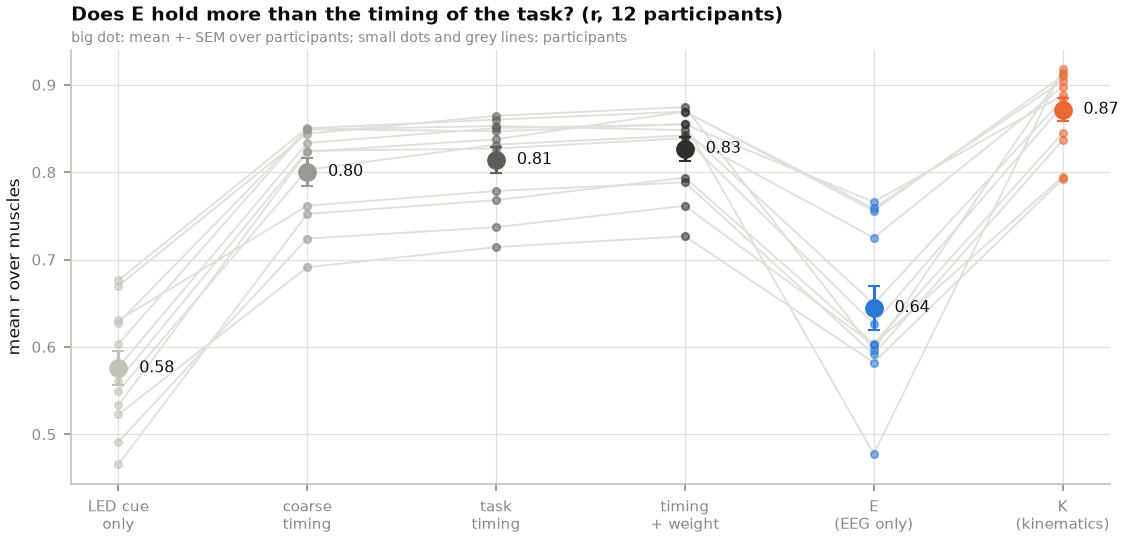
\includegraphics[height=52mm,width=\linewidth,keepaspectratio]{ctrl_A1_phase_vs_E_r.png}}
    \FigCap{Mean $r$ over muscles; grey lines: participants. Task-timing models (no EEG) vs E and K.}
    \column{0.45\linewidth}
    \begin{itemize}\scriptsize
      \item \textbf{phase}: linear model that only knows the times of the task events: $r$ \alert{0.814}, better than E
            (0.645) in \alert{12 of 12}; same muscle ranking as E.
      \item \textbf{cue}: only the LED time: $r$ 0.576, about 90\% of E.
      \item Beta ERD is classic in all 12; its top-3 electrodes (C3, CP1, C4) are E's top 3. But E also reads frontal-pole and neck electrodes.
      \item Causal v2 (predict 0--1000 ms ahead): F$-$K $+0.55$ VAF at 500 ms, only in the reach phase.
    \end{itemize}
    \begin{tcolorbox}[notebox,title={Reading}]
      What EEG knows about the muscles is contained in the task timing, and it knows even that less precisely than the event times themselves; it adds nothing beyond timing.
    \end{tcolorbox}
  \end{columns}
  \Verify{\scriptsize The phase model sees the future event times, so it is a ceiling, not a fair competitor. Is a causal timing baseline (past events only) the right reference instead?}
\end{frame}

\begin{frame}{Control A: per muscle, and what the timing model predicts}
  \begin{columns}[T]
    \column{0.52\linewidth}
    \FigRow{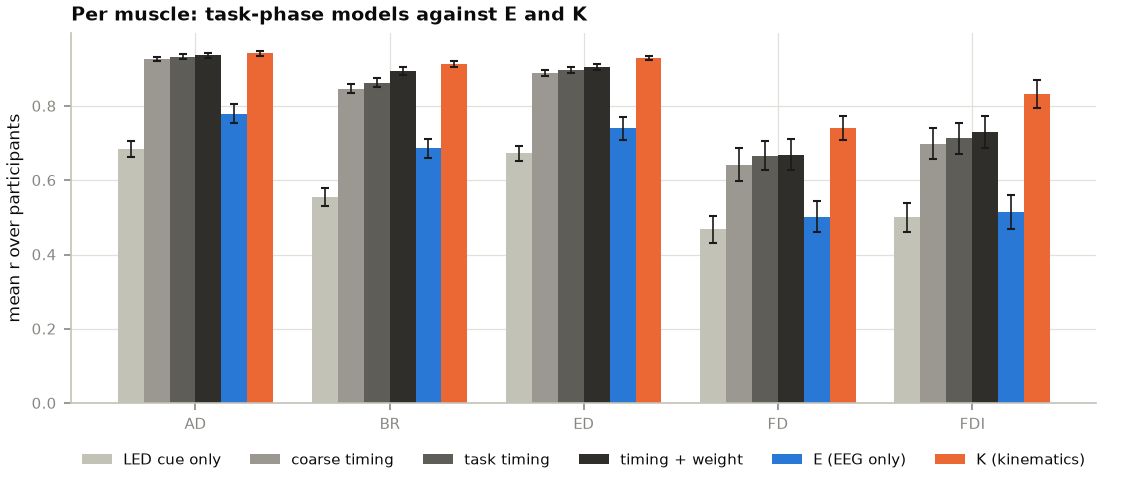
\includegraphics[width=\linewidth,height=30mm,keepaspectratio]{ctrl_A3_phase_per_muscle.png}}
    \FigCap{The same comparison per muscle (mean of 12 $\pm$ SEM).}
    \begin{itemize}\scriptsize
      \item The muscle ranking of E (shoulder best, fingers worst) is exactly the ranking of the timing model: it need
            not come from the brain.
      \item Correlation of E's and phase's accuracy across participants is only 0.38.
    \end{itemize}
    \column{0.44\linewidth}
    \FigRow{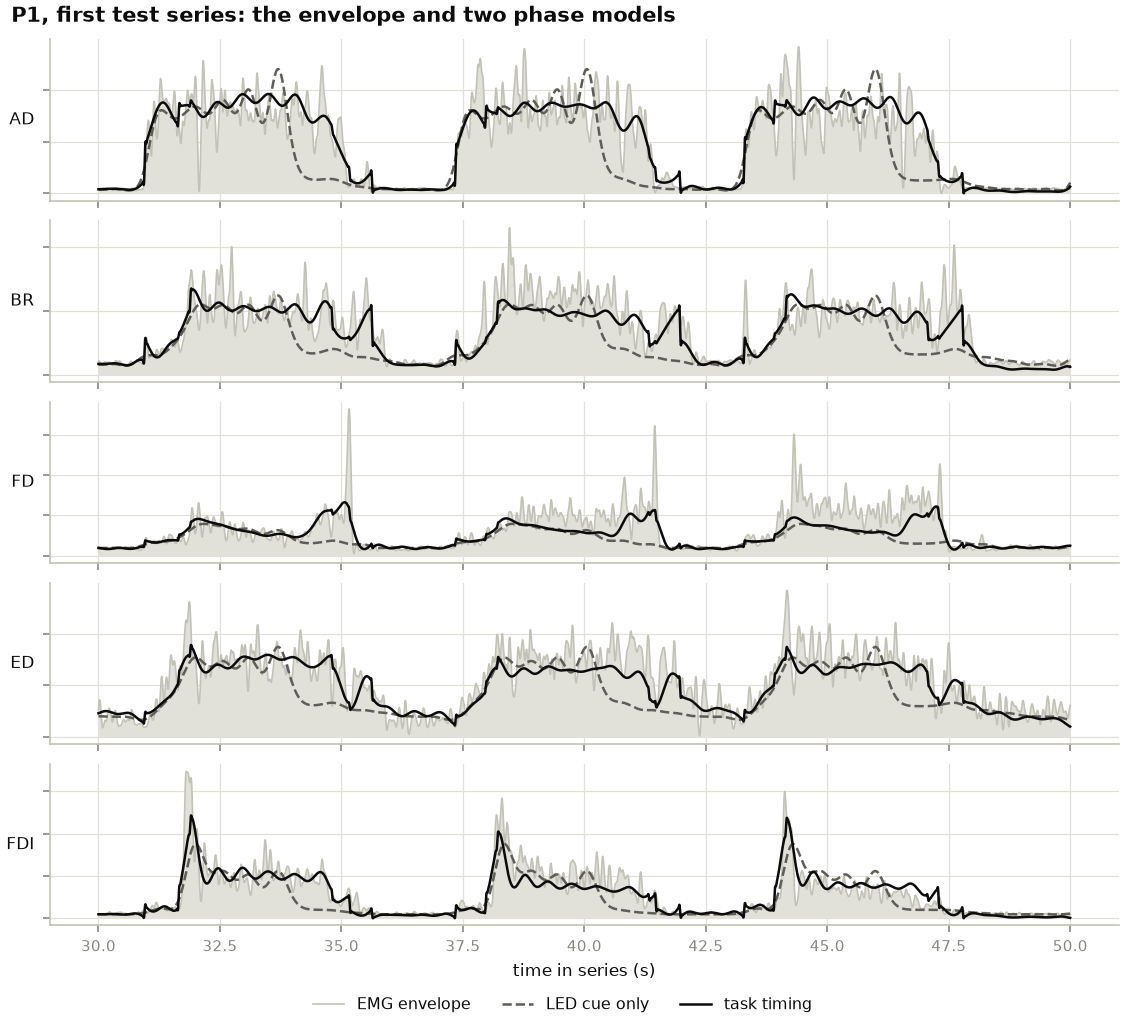
\includegraphics[width=\linewidth,height=56mm,keepaspectratio]{ctrl_A4_phase_example.png}}
    \FigCap{20 s of P1: true envelope (grey), cue model (dashed), phase model (black).}
  \end{columns}
\end{frame}

\begin{frame}{Control B: classic reference maps (group of 12)}
  \FigRow{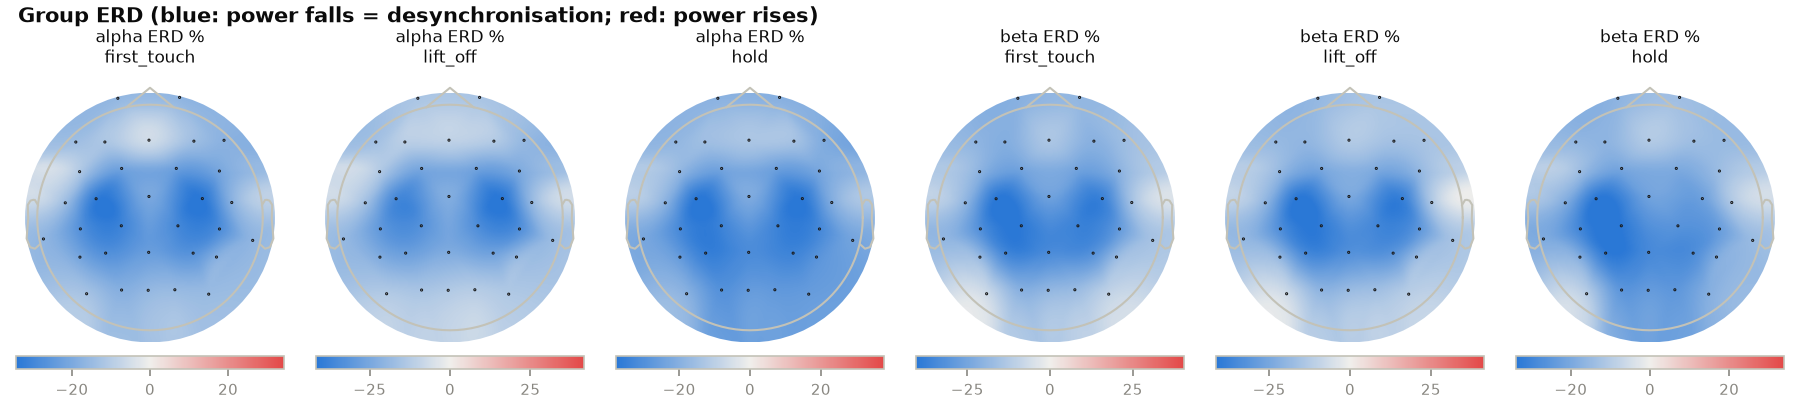
\includegraphics[width=\textwidth,height=23mm,keepaspectratio]{ctrl_B1_group_erd.png}}
  \FigCap{Group ERD (blue: power decrease from rest). Focus over C3, C4 and CP electrodes in all six maps.}
  \vspace{1mm}
  \FigRow{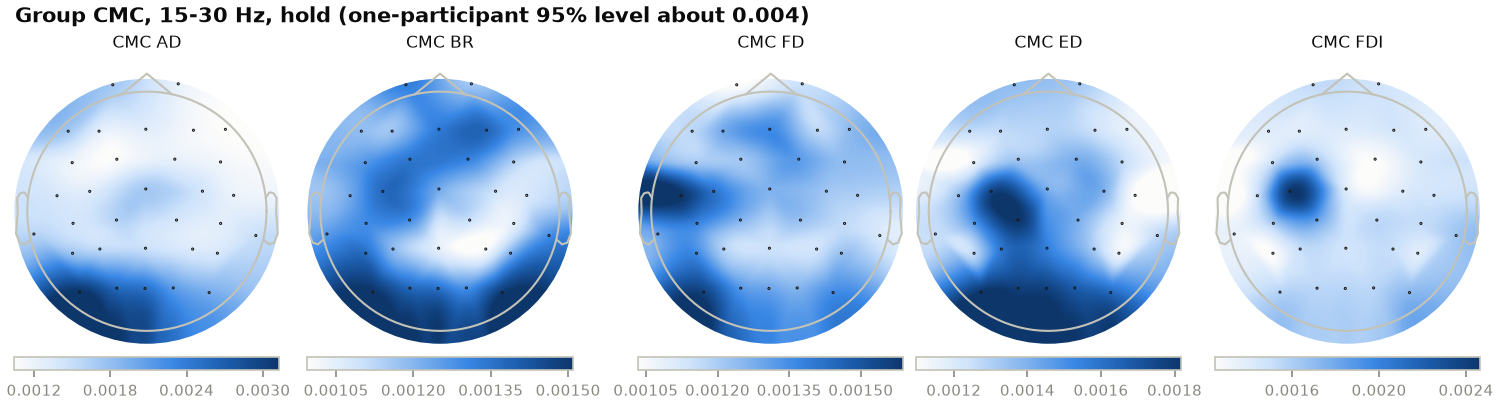
\includegraphics[width=\textwidth,height=23mm,keepaspectratio]{ctrl_B2_group_cmc.png}}
  \FigCap{Group beta CMC during the hold, per muscle (own colour scale each).}
  \begin{itemize}\scriptsize
    \item ERD is classic in every participant: the top 8 electrodes lose beta power in all 12.
    \item CMC is weak in this data (group values below one participant's significance level) and focuses on the back
          of the head for most muscles: a contaminated reference.
  \end{itemize}
\end{frame}

\begin{frame}{Control B: does E's map agree with the reference maps?}
  \begin{columns}[T]
    \column{0.49\linewidth}
    \FigRow{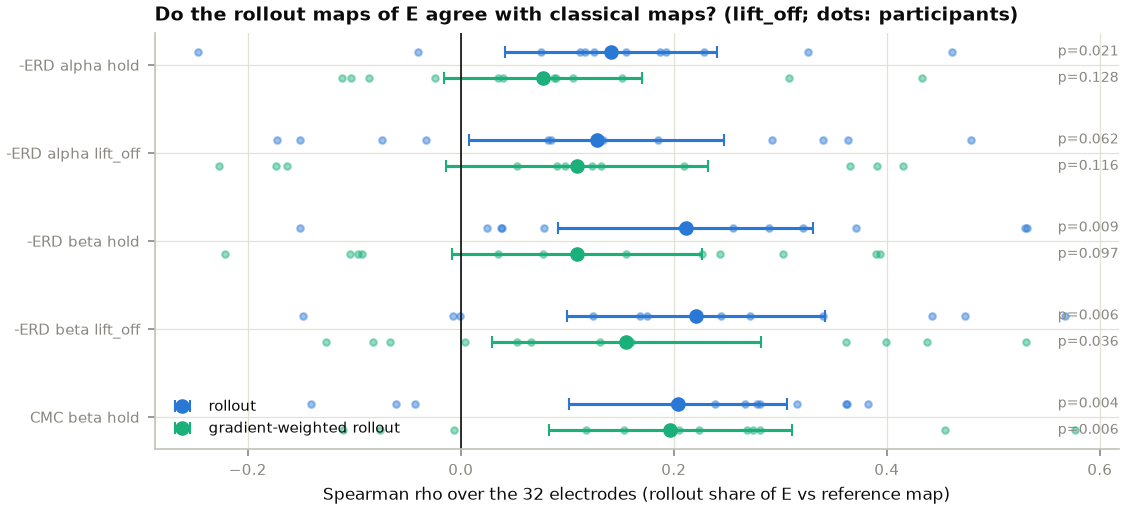
\includegraphics[width=\linewidth,height=34mm,keepaspectratio]{ctrl_B3_rollout_vs_reference_lift_off.png}}
    \FigCap{Spearman $\rho$ of E's map with each reference; dots: participants.}
    \begin{itemize}\scriptsize
      \item With beta ERD: $\rho$ 0.22 ($p$ 0.006, positive in 9 of 12).
      \item With CMC: 0.20 ($p$ 0.004); 0.52 on the group map.
      \item Significant but moderate.
    \end{itemize}
    \column{0.49\linewidth}
    \FigRow{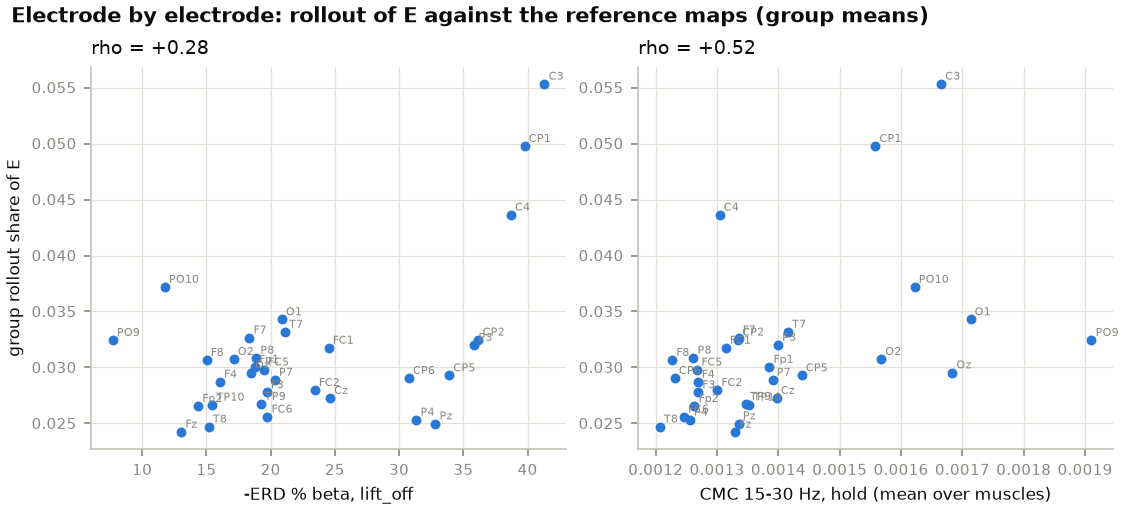
\includegraphics[width=\linewidth,height=34mm,keepaspectratio]{ctrl_B5_electrode_scatter.png}}
    \FigCap{One dot per electrode: E's share against the reference.}
    \begin{itemize}\scriptsize
      \item C3, CP1, C4: high in both (sensorimotor).
      \item PO9, PO10, O1, F7, T7: read by E, little ERD (neck muscles, eye, temporal muscle).
      \item Pz, P4, CP5: strong ERD, not read by E.
    \end{itemize}
  \end{columns}
\end{frame}

\begin{frame}{Control C: a causal v2, predicting ahead}
  \FigRow{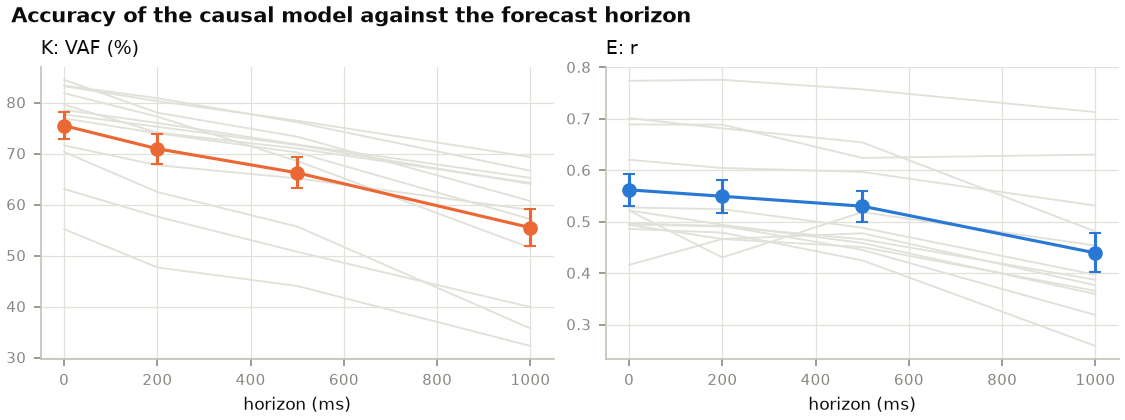
\includegraphics[width=0.49\textwidth,height=30mm,keepaspectratio]{ctrl_C2_accuracy_vs_horizon.png}\hspace{2mm}%
          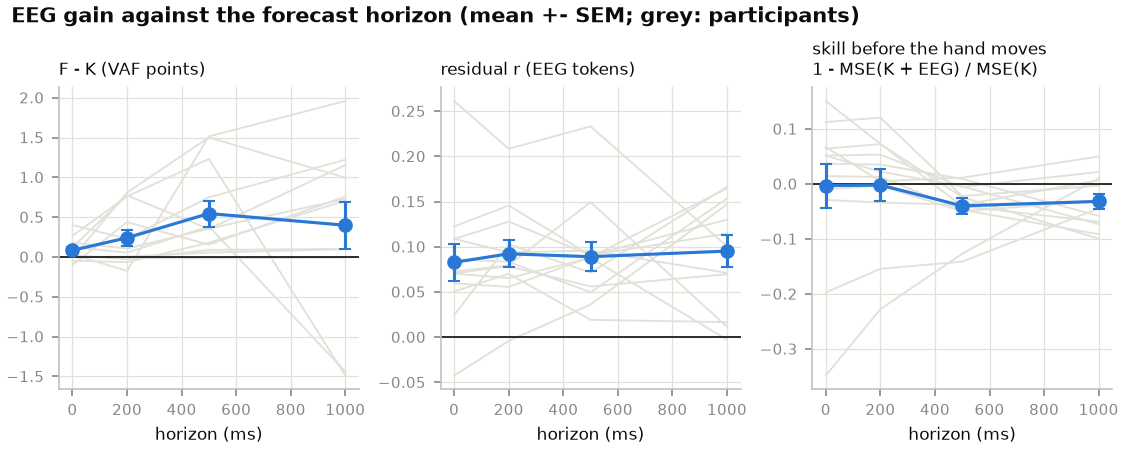
\includegraphics[width=0.49\textwidth,height=30mm,keepaspectratio]{ctrl_C1_eeg_gain_vs_horizon.png}}
  \FigCap{Left: accuracy vs horizon (K VAF, E $r$). Right: F$-$K, residual-test $r$, ridge skill before movement.}
  \begin{columns}[T]
    \column{0.48\linewidth}
    \begin{itemize}\scriptsize
      \item Causal K at 0 ms: VAF 75.5\% (offline 75.8\%). Causal E weaker: $r$ 0.56 vs 0.64.
      \item K falls fast with the horizon (55.5\% at 1 s); E's $r$ is flat to 500 ms, 0.44 at 1 s.
    \end{itemize}
    \column{0.48\linewidth}
    \begin{itemize}\scriptsize
      \item F$-$K: $+0.08$, $+0.24$, $+0.55$ (11 of 12, $p$ 0.0005), $+0.40$ (n.s.) VAF points.
      \item Residual $r$ flat at 0.08--0.10; with raw band power it \emph{falls} with the horizon.
      \item Ridge skill in the second before movement is never positive.
    \end{itemize}
  \end{columns}
\end{frame}

\begin{frame}{Control C: per task phase}
  \FigRow{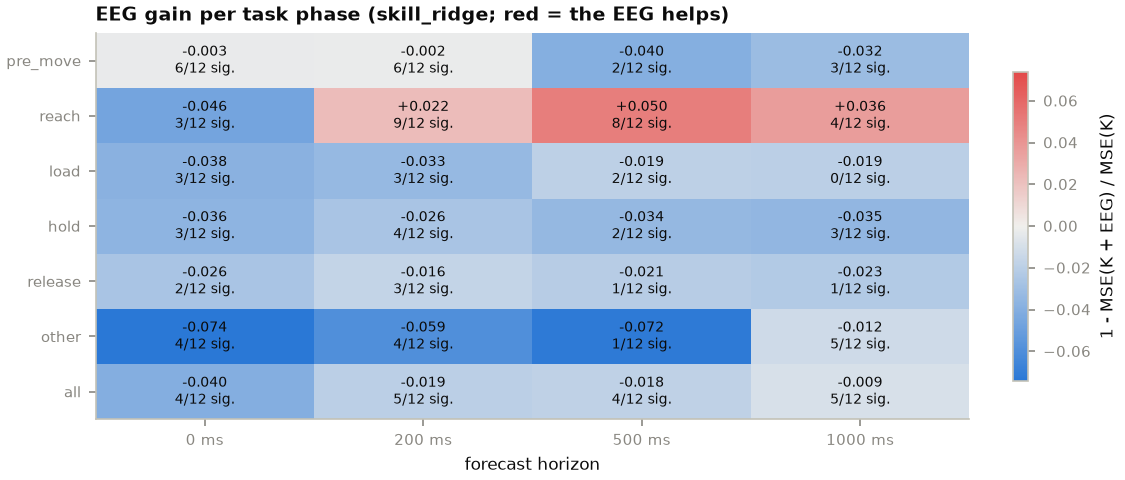
\includegraphics[width=0.49\textwidth,height=32mm,keepaspectratio]{ctrl_C3_gain_per_phase_ridge.png}\hspace{2mm}%
          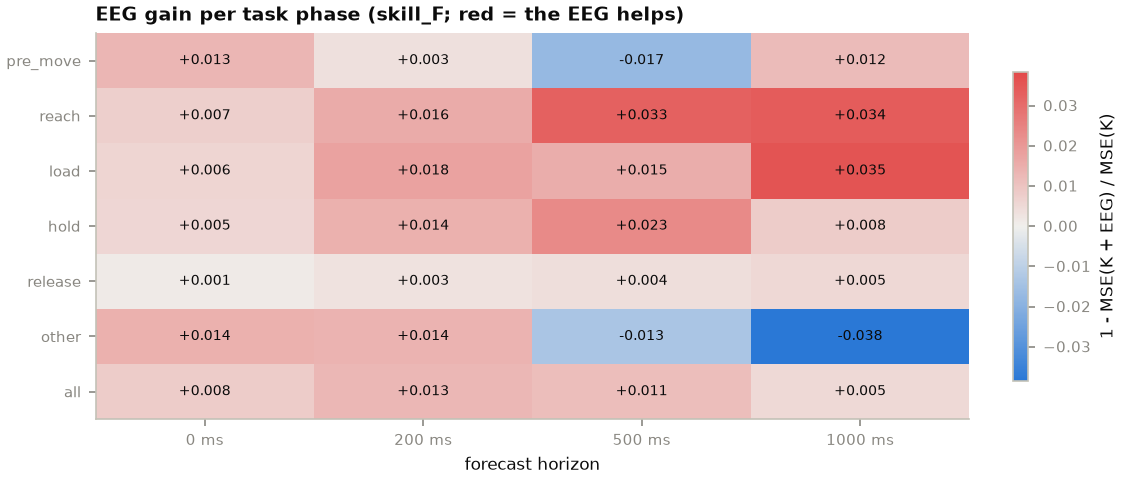
\includegraphics[width=0.49\textwidth,height=32mm,keepaspectratio]{ctrl_C4_gain_per_phase_F.png}}
  \FigCap{Skill per phase and horizon (red: EEG reduces K's error). Left: external ridge. Right: the model's own F.}
  \begin{itemize}\scriptsize
    \item Before movement, the EEG's correlation with K's error grows with the horizon: 0.06 $\to$ 0.19 ($p$ 0.008).
    \item Real error reduction only in the reach phase: up to 5\%; about half of it remains when the prediction is
          shifted in time (null $+0.026$), so the time-locked part is 0.02--0.03.
    \item F's own correction is small and positive in 25 of 28 cells (up to $+0.035$).
    \item Caution: before movement K's error is mostly "when does the movement start?", which the EEG may know from
          the LED response, not from a motor command.
  \end{itemize}
\end{frame}

%% =============================================================
\section{v3: EEG as the base, kinematics as a guide}
%% =============================================================

\begin{frame}{v3: one fair comparison, and the team's proposal}
  \small
  Review of v2 by the team: \emph{the EEG should be the base; kinematics may only help during training.}
  The team's proposal (critical experiment II) turned this into one fair comparison.

  \medskip
  \centering\scriptsize
  \begin{tabular}{lll}
    \toprule
    condition & input at time $t$ & role \\
    \midrule
    causal\_cue & past LED and event times & task timing only \\
    K & past kinematics and force & biomechanical explanation \\
    \textbf{B} & K + past task events & \textbf{primary no-EEG baseline} \\
    \textbf{F} & B + EEG history & \textbf{primary neural candidate} \\
    E0 & EEG only, no guide & EEG-only reference \\
    Eguided & EEG only, frozen K teacher in training & secondary intervention \\
    \bottomrule
  \end{tabular}

  \medskip
  \raggedright
  \textbf{Primary metric:} $\text{eeg\_skill}=1-\mathrm{MSE}(F)/\mathrm{MSE}(B)$, horizons 0, 200, 500, 1000 ms, Wilcoxon over
  participants with Holm correction. \textbf{Controls on F:} EEG of another trial with all events aligned
  (phase\_swap), LED-aligned swap, band power, peripheral channels only, muscle-onset error.
\end{frame}

\begin{frame}{v3 run and training, step by step}
  \centering
  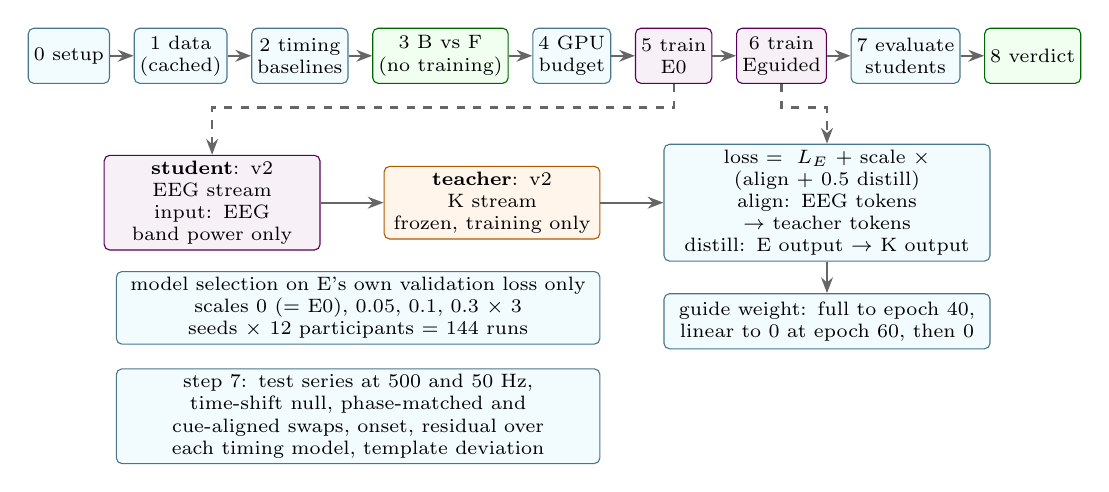
\begin{tikzpicture}[node distance=2.5mm and 3mm]
    \node[blk] (s0) {0 setup};
    \node[blk,right=of s0] (s1) {1 data\\(cached)};
    \node[blk,right=of s1] (s2) {2 timing\\baselines};
    \node[good,right=of s2] (s3) {3 B vs F\\(no training)};
    \node[blk,right=of s3] (s4) {4 GPU\\budget};
    \node[eeg,right=of s4] (s5) {5 train\\E0};
    \node[eeg,right=of s5] (s6) {6 train\\Eguided};
    \node[blk,right=of s6] (s7) {7 evaluate\\students};
    \node[good,right=of s7] (s8) {8 verdict};
    \foreach \a/\b in {s0/s1,s1/s2,s2/s3,s3/s4,s4/s5,s5/s6,s6/s7,s7/s8} \draw[arr] (\a)--(\b);

    \node[eeg,text width=26mm,below=9mm of s1,xshift=4mm] (st) {\textbf{student}: v2 EEG stream\\input: EEG band power only};
    \node[kin,text width=26mm,right=8mm of st] (te) {\textbf{teacher}: v2 K stream\\frozen, training only};
    \node[blk,text width=40mm,right=8mm of te] (gd) {loss $=L_E$ + scale $\times$ (align + 0.5 distill)\\align: EEG tokens $\to$ teacher tokens\\distill: E output $\to$ K output};
    \draw[arr] (st)--(te); \draw[arr] (te)--(gd);
    \node[blk,text width=40mm,below=4mm of gd] (sc) {guide weight: full to epoch 40,\\linear to 0 at epoch 60, then 0};
    \node[blk,text width=60mm,below=4mm of te,xshift=-17mm] (sel) {model selection on E's own validation loss only\\scales 0 (= E0), 0.05, 0.1, 0.3 $\times$ 3 seeds $\times$ 12 participants $=$ 144 runs};
    \draw[arr] (gd)--(sc);
    \draw[arr,dashed] (s5.south) -- ++(0,-3mm) -| (st.north);
    \draw[arr,dashed] (s6.south) -- ++(0,-3mm) -| (gd.north);
    \node[blk,text width=60mm,below=3mm of sel] (ev) {step 7: test series at 500 and 50 Hz, time-shift null, phase-matched and cue-aligned swaps, onset, residual over each timing model, template deviation};
  \end{tikzpicture}
  \FigCap{After epoch 60 every guided run is pure EEG $\to$ EMG; at test time the student never sees kinematics.}
  \Verify{\scriptsize Is a maximum guide scale of 0.3, faded out by epoch 60, too weak a test of the guide idea?}
\end{frame}

\begin{frame}{v3 step 2: causal timing baselines}
  \FigRow{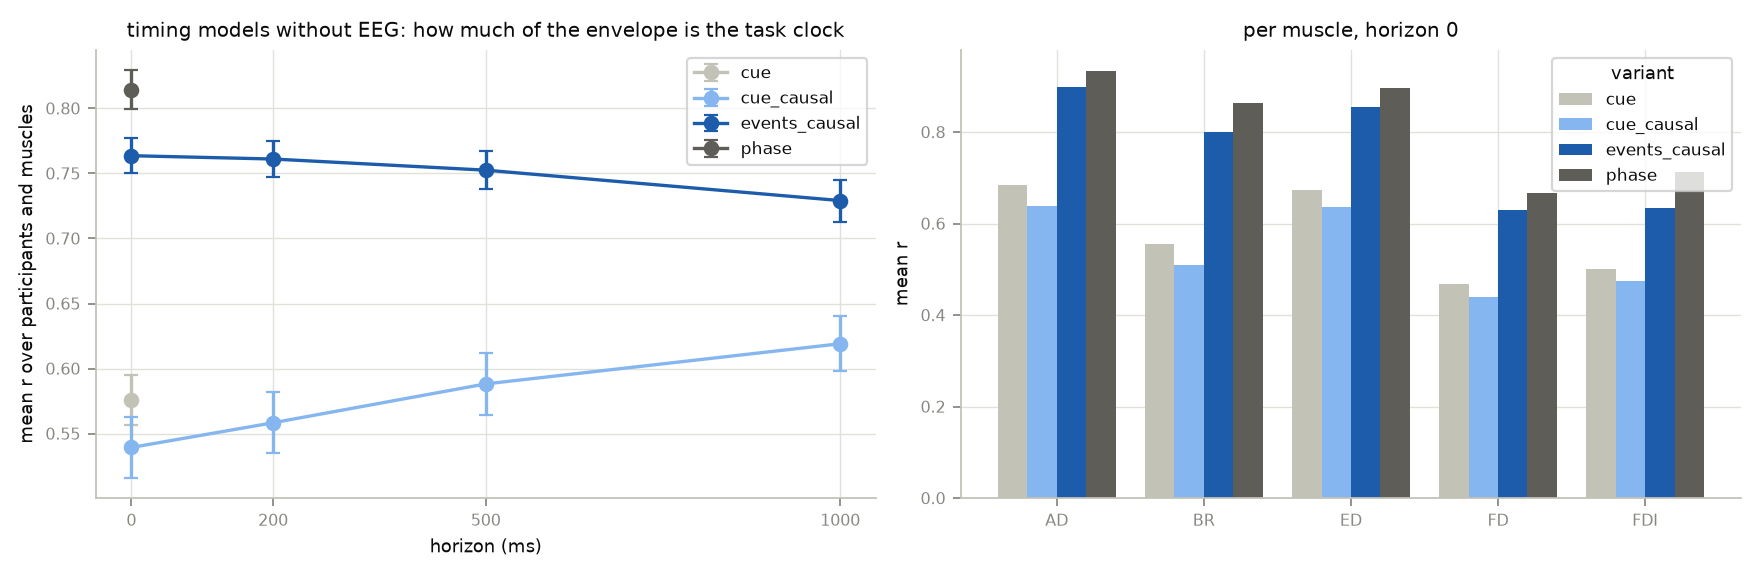
\includegraphics[width=\textwidth,height=40mm,keepaspectratio]{v3_timing.png}}
  \FigCap{Models without EEG. Left: mean $r$ vs horizon. Right: per muscle at 0 ms.}
  \centering\scriptsize
  \begin{tabular}{lcccc}
    \toprule
    model & 0 ms & 200 ms & 500 ms & 1000 ms \\
    \midrule
    causal\_cue (past LED only) & 0.539 & 0.558 & 0.588 & 0.619 \\
    events\_causal (past events) & 0.764 & 0.761 & 0.753 & 0.729 \\
    phase / cue (see the future, ceilings) & 0.814 / 0.576 & --- & --- & --- \\
    \bottomrule
  \end{tabular}
  \FigCap{Even the causal past-events model beats the EEG-only model (0.63). Muscle order: shoulder better than fingers, as in E.}
\end{frame}

\begin{frame}{Primary result: F never beats B}
  \begin{columns}[T]
    \column{0.50\linewidth}
    \FigRow{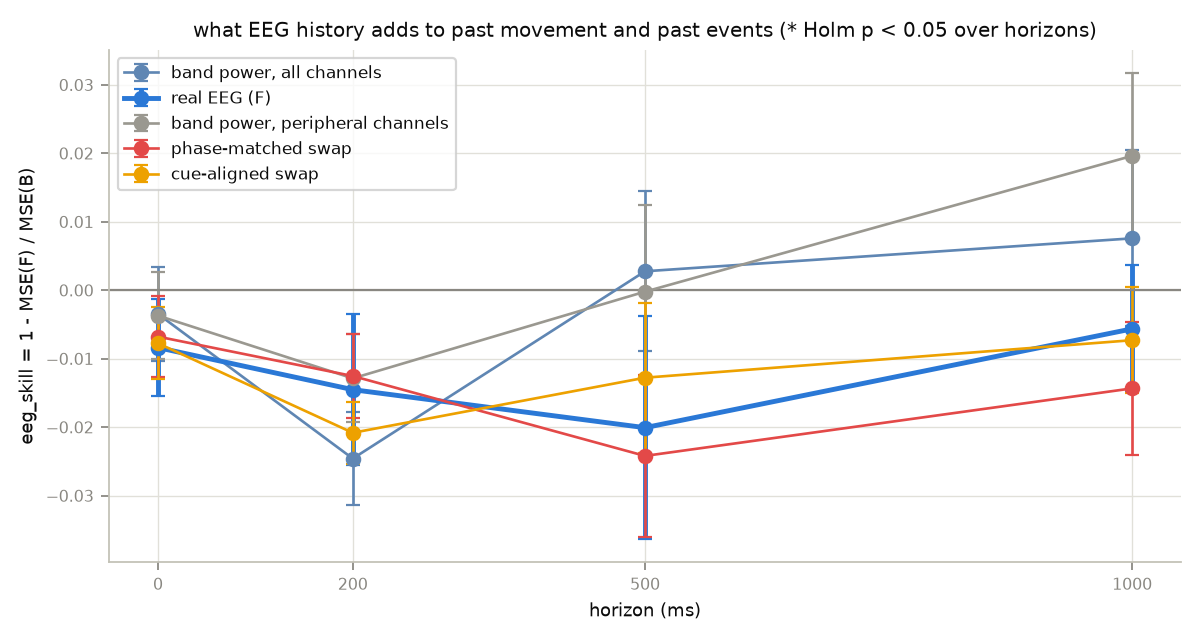
\includegraphics[height=50mm,width=\linewidth,keepaspectratio]{v3_bvsf_horizon.png}}
    \column{0.47\linewidth}
    \centering\scriptsize
    \begin{tabular}{lccc}
      \toprule
      horizon & eeg\_skill & $p$ (Holm) & significant in \\
      \midrule
      0 ms & $-0.008$ & 1.00 & 2 of 12 \\
      200 ms & $-0.015$ & 1.00 & 3 of 12 \\
      500 ms & $-0.020$ & 1.00 & 2 of 12 \\
      1000 ms & $-0.006$ & 1.00 & 3 of 12 \\
      \bottomrule
    \end{tabular}
    \raggedright
    \begin{itemize}\scriptsize
      \item F's error is 0.6--2.0\% \emph{larger} than B's.
      \item EEG from another trial and peripheral band power give the same result; no task phase is significant.
      \item B beats K by 2--3\% at 200 and 500 ms and predicts muscle onset better (500 ms: 400 $\to$ 240 ms).
      \item The small v2 gain at 500 ms disappears once past events enter the baseline.
    \end{itemize}
  \end{columns}
  \Verify{\scriptsize B and F ridges are fitted on one validation series only (K was trained on the training series). Is a cross-validated fit on test trials needed as a sensitivity check?}
\end{frame}

\begin{frame}{v3 step 3: per phase and per participant}
  \FigRow{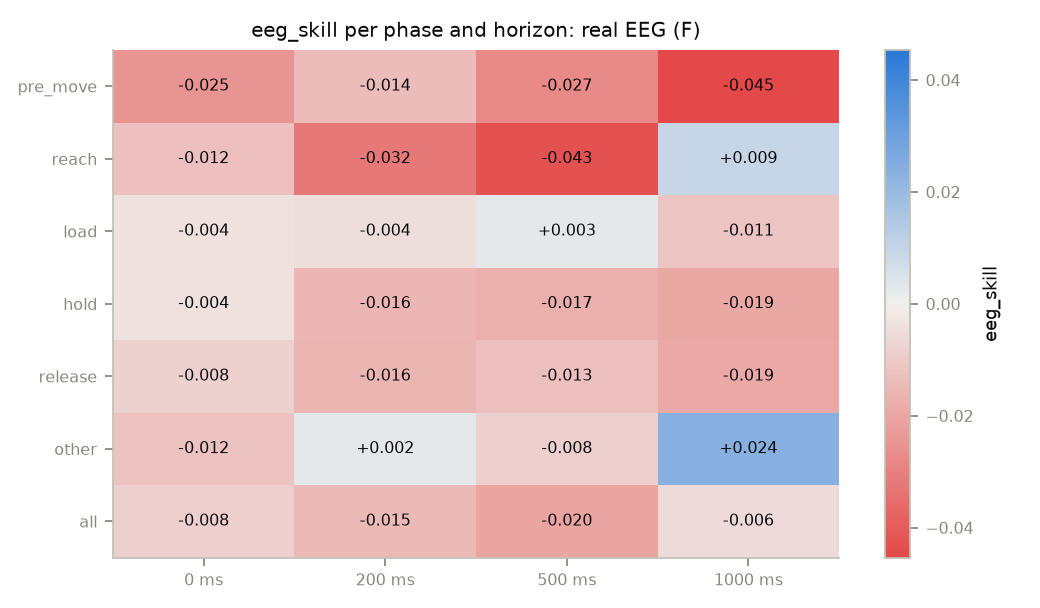
\includegraphics[width=0.45\textwidth,height=44mm,keepaspectratio]{v3_bvsf_phases.png}\hspace{3mm}%
          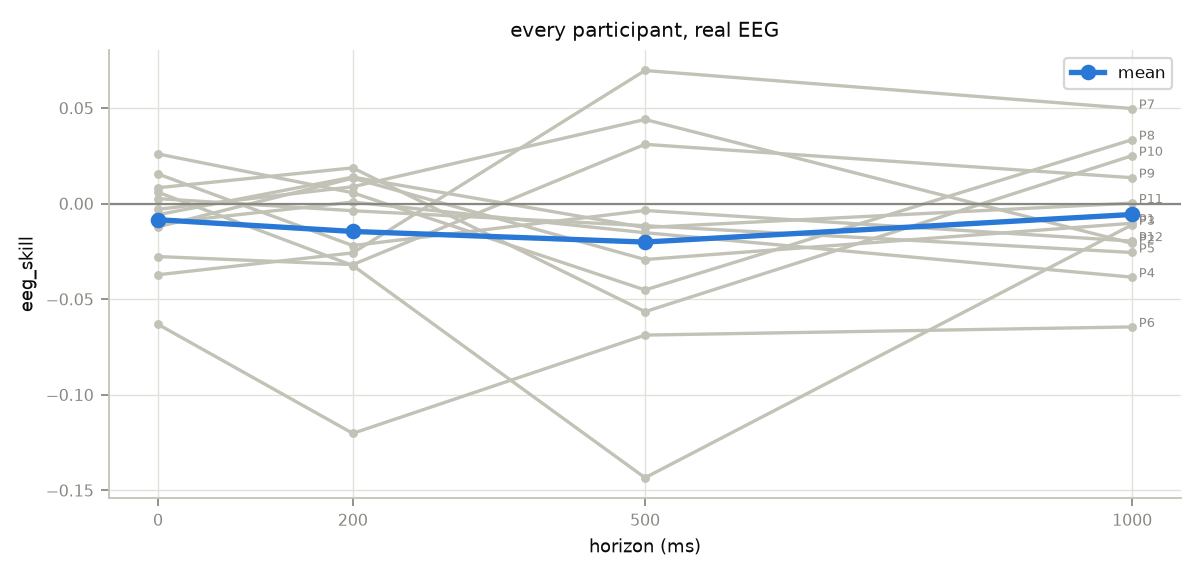
\includegraphics[width=0.50\textwidth,height=44mm,keepaspectratio]{v3_bvsf_participants.png}}
  \FigCap{Left: eeg\_skill of F per task phase and horizon; a star would mean significant after Holm over phases, none has one.
          Right: eeg\_skill per participant (grey) and mean (blue).}
\end{frame}

\begin{frame}{v3 step 3: the error ladder and muscle onset}
  \FigRow{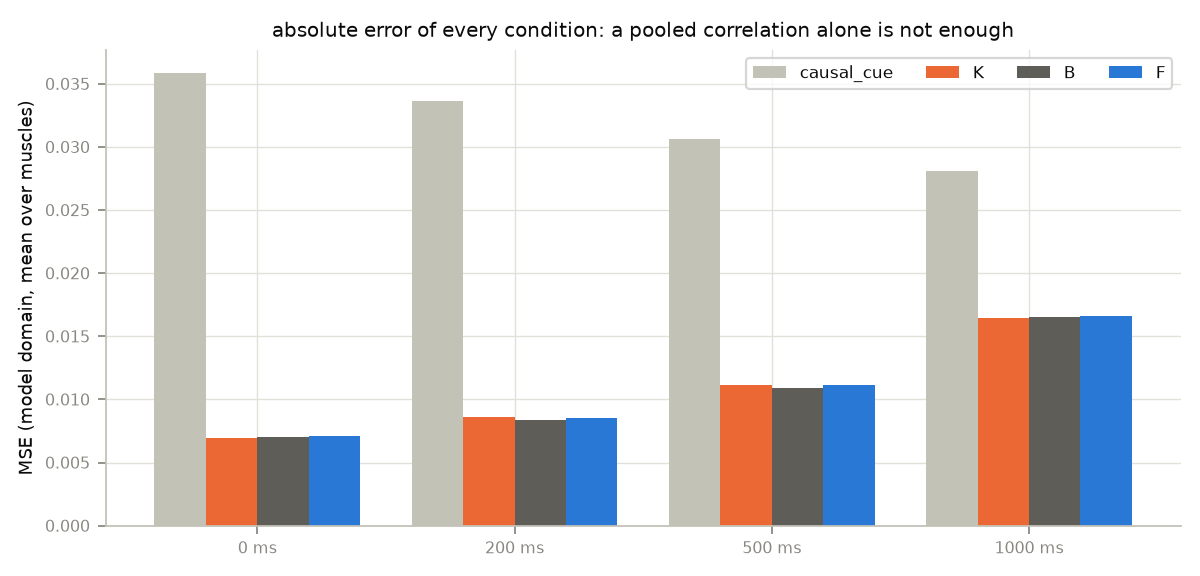
\includegraphics[width=0.49\textwidth,height=40mm,keepaspectratio]{v3_mse_ladder.png}\hspace{2mm}%
          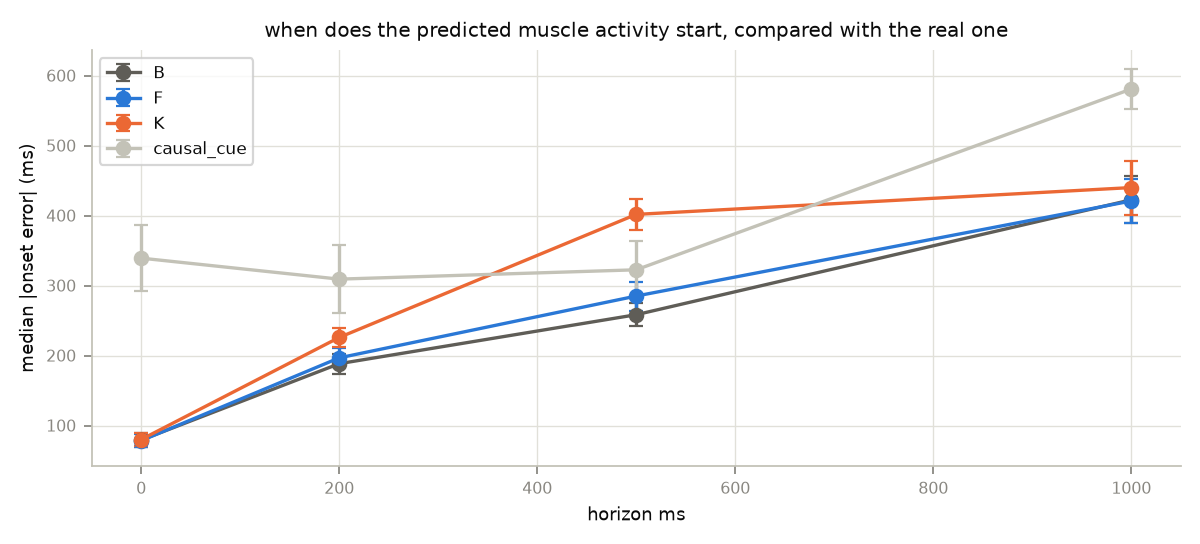
\includegraphics[width=0.49\textwidth,height=40mm,keepaspectratio]{v3_onset.png}}
  \FigCap{Left: absolute error of causal\_cue, K, B and F per horizon. Right: median absolute onset error per condition.}
  \begin{itemize}\scriptsize
    \item Each step down the ladder (timing $\to$ K $\to$ B) reduces the error; the EEG step (B $\to$ F) does not.
    \item Onset (envelope first reaches 20\% of its range after the cue): B is better than K at 200 and 500 ms
          (500 ms: 400 $\to$ 240 ms); F equals B.
  \end{itemize}
\end{frame}

\begin{frame}{v3 steps 5--6: training curves of all 144 runs}
  \FigRow{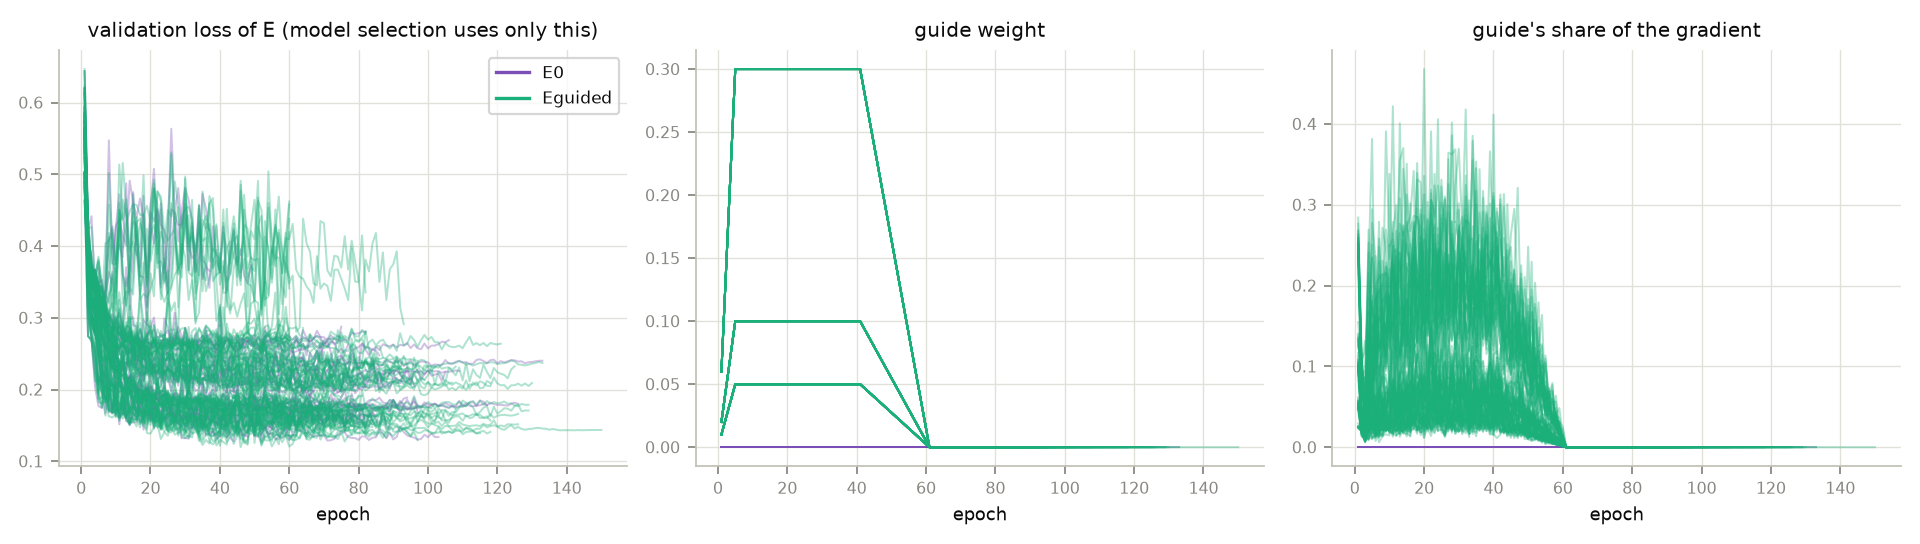
\includegraphics[width=\textwidth,height=40mm,keepaspectratio]{v3_training.png}}
  \FigCap{Left: E's own validation loss (the only selection criterion). Middle: guide weight. Right: guide share of the gradient.}
  \begin{itemize}\scriptsize
    \item The guide is active until epoch 60, then every run is pure EEG $\to$ EMG.
    \item Validation loss of the guided runs is practically equal to E0: the largest change is $-0.83\%$ at scale 0.3,
          lower in 7 of 12, $p$ 0.10.
  \end{itemize}
\end{frame}

\begin{frame}{Secondary result: the guide does not help, and E is task-locked}
  \begin{columns}[T]
    \column{0.48\linewidth}
    \textbf{Test series, mean of 12 (3 seeds each)}

    \smallskip
    \centering\scriptsize
    \begin{tabular}{lccc}
      \toprule
      model & $r$ & gain & $p$ (Holm) \\
      \midrule
      E0 & 0.633 & & \\
      Eguided 0.05 & 0.635 & +0.002 & 0.40 \\
      Eguided 0.1 & 0.634 & +0.002 & 0.30 \\
      Eguided 0.3 & 0.641 & +0.008 & 0.26 \\
      \bottomrule
    \end{tabular}
    \raggedright
    \begin{itemize}\scriptsize
      \item Same picture in validation ($-0.83$\% loss, $p$ 0.10).
      \item E0 is worse than the phase model in 12 of 12.
    \end{itemize}
    \column{0.48\linewidth}
    \begin{tcolorbox}[stagebox,title={The strongest single number}]
      \scriptsize
      E0 with the EEG of \textbf{another trial}, all task events aligned:\\
      $r$ 0.633 $\to$ \alert{0.571}: it keeps \alert{90\%} of its accuracy.\\[2pt]
      The remaining 10\% is real (drop in 12 of 12), but it explains nothing of the phase model's residual
      (skill 0.001, null 0.002, $p$ 0.69).
    \end{tcolorbox}
    \vspace{2pt}
    \begin{tcolorbox}[notebox,title={Verdict (step 8), every horizon}]
      F beats B: \textbf{no} \quad Eguided beats E0: \textbf{no}\\
      $\Rightarrow$ \emph{no evidence that EEG adds information beyond movement and timing.}
    \end{tcolorbox}
  \end{columns}
\end{frame}

%% =============================================================
\section{Prediction-error pilot}
%% =============================================================

\begin{frame}{Why we ran this pilot}
  \begin{columns}[T]
    \column{0.50\linewidth}
    \textbf{Where v3 left us}
    \begin{itemize}\scriptsize
      \item EEG $\to$ EMG is closed: with movement and timing known, EEG adds nothing, and the EEG-only model keeps
            90\% of its accuracy with another trial's EEG.
      \item Before deciding between ``continue'' and ``audit'', we asked whether the \emph{same data} holds a different
            neural question worth a paper.
    \end{itemize}
    \textbf{Why prediction error}
    \begin{itemize}\scriptsize
      \item The task was designed for it: the weight changes without warning (Johansson \& Westling), so the brain's
            prediction of the object is wrong on 76 lifts per participant.
      \item The claim would not need EEG to beat kinematics: it asks whether the brain \emph{responds} to the error,
            a classic event-locked question.
      \item The dataset paper showed it for one participant (P3), no statistical test; we found no group-level,
            movement-controlled study.
    \end{itemize}
    \column{0.46\linewidth}
    \begin{tcolorbox}[stagebox,title={Why it was cheap to test}]
      \scriptsize No training, the raw files only, one afternoon of compute. Pass/fail criteria fixed in the notebook
      before any result was seen.
    \end{tcolorbox}
    \begin{tcolorbox}[notebox,title={What a ``go'' would have looked like}]
      \scriptsize
      \begin{itemize}
        \item an EEG cluster over sensorimotor channels that starts \emph{before} force and EMG differ, or
        \item the expected weight decodable from EEG before the hand touches the object (nothing physical differs yet)
      \end{itemize}
      Either one would be a neural claim that the movement cannot explain.
    \end{tcolorbox}
  \end{columns}
\end{frame}

\begin{frame}{Pilot: the design}
  \begin{columns}[T]
    \column{0.50\linewidth}
    \textbf{Why}
    \begin{itemize}\scriptsize
      \item The task was built for it: the weight changes without warning, so the grip force planned from the last
            lift is wrong.
      \item 38 heavier and 38 lighter lifts per participant (165, 330, 660 g).
      \item The dataset paper showed the EEG effect for one participant (P3) only, without a statistical test.
    \end{itemize}
    \textbf{Labels}
    \begin{itemize}\scriptsize
      \item \textbf{expected}: same weight as the lift before; \textbf{heavier}; \textbf{lighter}
      \item no label for the first lift of a series and for lifts where the surface changed too
    \end{itemize}
    \column{0.46\linewidth}
    \begin{tcolorbox}[stagebox,title={Key control: same object, different expectation}]
      \scriptsize 660 g after 165 g (unexpected) vs 660 g after 660 g (expected). Difference taken within each current
      weight, then averaged. Participant is the unit of every test.
    \end{tcolorbox}
    \begin{tcolorbox}[notebox,title={Four analyses, no training}]
      \scriptsize
      1. behaviour (sanity check of the labels)\\
      2. error response: EEG, EMG and force on one time axis, cluster permutation\\
      3. expectation before contact: decoder of the previous weight, with EMG, hand-speed, pre-cue and peripheral controls\\
      4. error size vs next-lift force update (exploratory)
    \end{tcolorbox}
    {\scriptsize Pass/fail criteria were fixed before the results. EEG peak-to-peak is about 300 $\mu$V per lift, so
    rejection is relative (median + 3 robust SD): 3--26 of 294 lifts per participant.\par}
  \end{columns}
\end{frame}

\begin{frame}{Pilot 1: behaviour confirms the labels}
  \FigRow{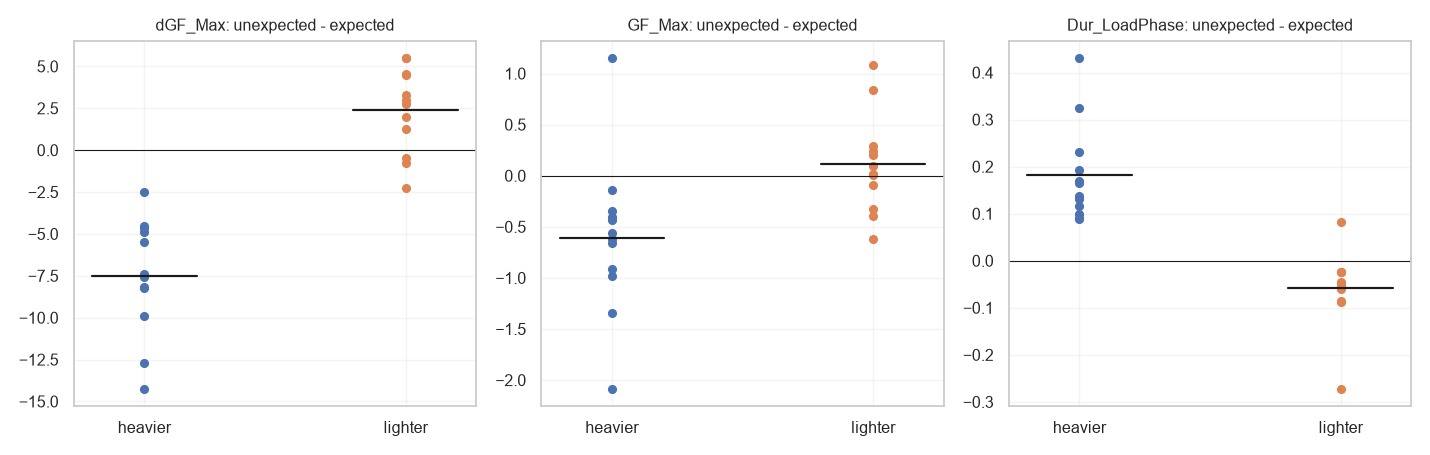
\includegraphics[width=\textwidth,height=36mm,keepaspectratio]{pe_behaviour.png}}
  \FigCap{Unexpected minus expected (same weight), one dot per participant.}
  \centering\scriptsize
  \begin{tabular}{llccc}
    \toprule
    & measure & mean difference & expected direction & $p$ \\
    \midrule
    heavier & load-phase duration & $+181$ ms & 12 of 12 & 0.0005 \\
    heavier & peak grip-force rate & $-7.5$ N/s & 12 of 12 & 0.0005 \\
    lighter & load-phase duration & $-58$ ms & 11 of 12 & 0.016 \\
    lighter & peak grip-force rate & $+2.4$ N/s & 9 of 12 & 0.012 \\
    \bottomrule
  \end{tabular}
  \FigCap{The classic Johansson and Westling effect: force is planned from the previous weight.}
\end{frame}

\begin{frame}{Pilot 2: error response, unexpectedly lighter}
  \begin{columns}[T]
    \column{0.44\linewidth}
    \FigRow{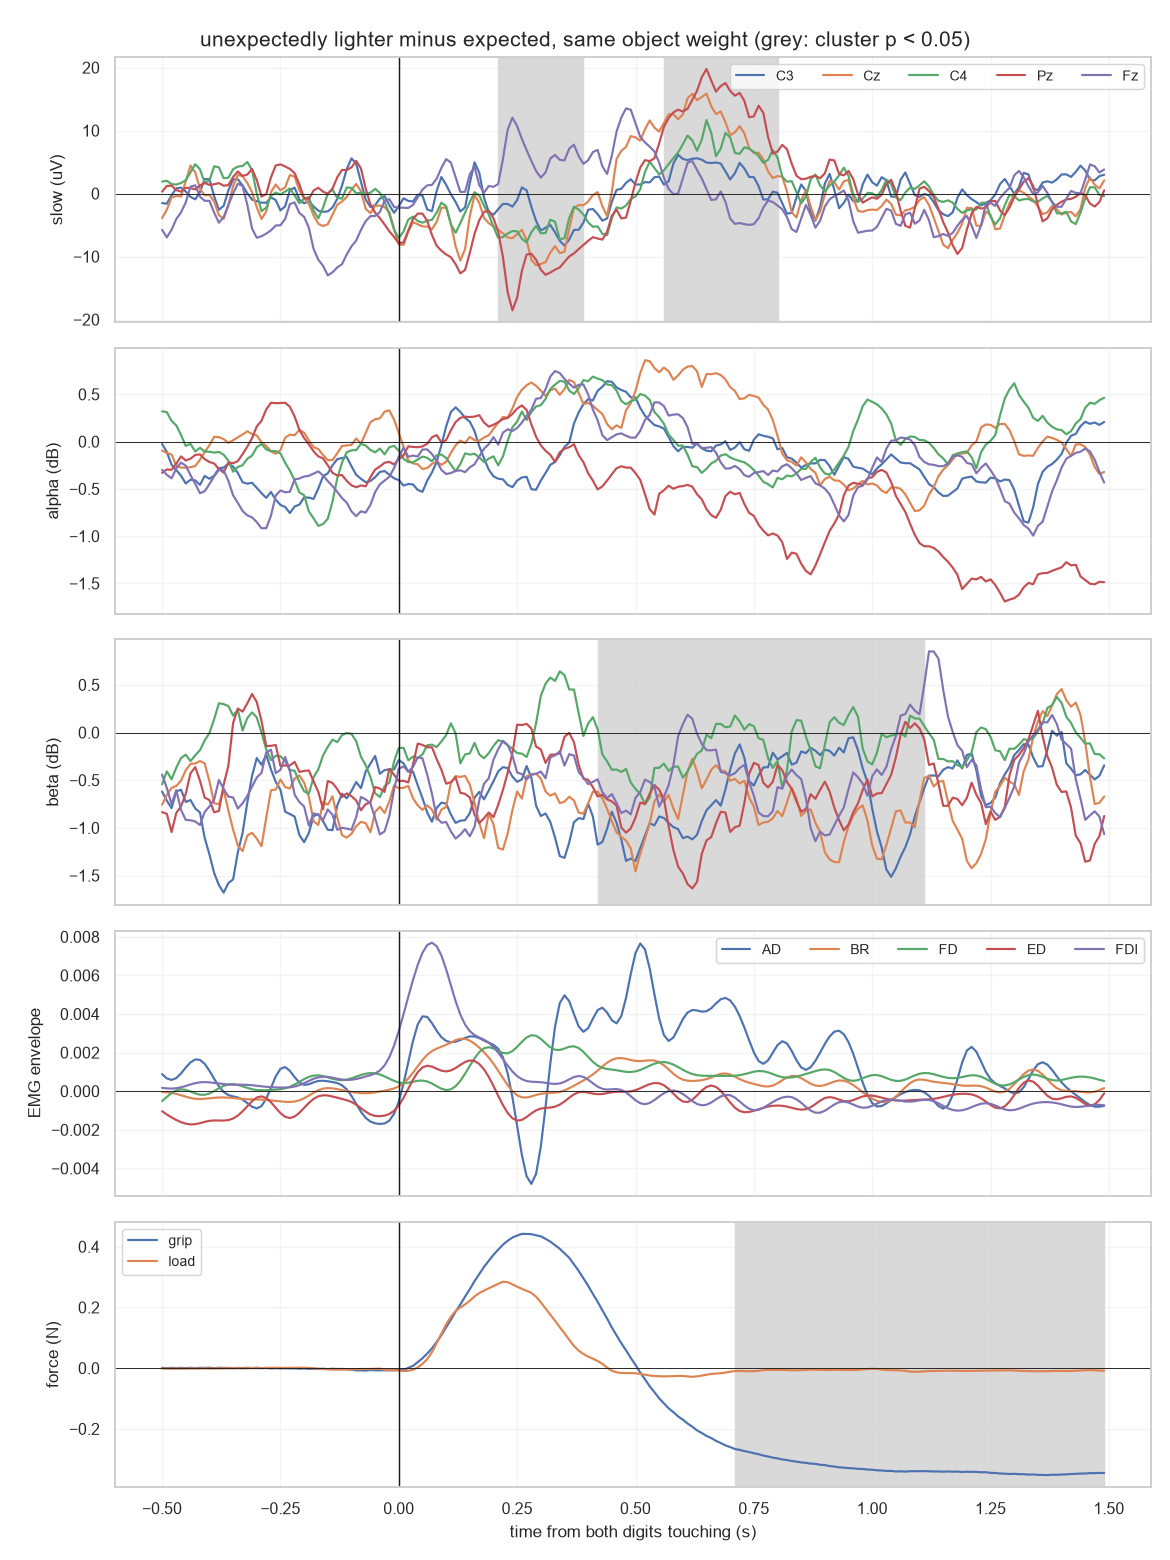
\includegraphics[height=68mm,width=\linewidth,keepaspectratio]{pe_error_lighter.png}}
    \column{0.52\linewidth}
    \FigCap{Group mean of 12, touch at 0 s. Rows: slow EEG, alpha, beta, EMG, grip and load force. Grey: clusters $p<0.05$.}
    \begin{itemize}\scriptsize
      \item Slow EEG: negative wave over C3, Cz, CP1, Pz at 210--390 ms ($p$ 0.027), then a positive wave at
            560--800 ms ($p$ 0.003).
      \item Beta power drops over left central channels from 420 ms ($p\approx0.04$).
      \item But grip and load force are already higher from about 60 ms (cluster $p\approx0.06$), and the lift-off
            time differs.
    \end{itemize}
    \begin{tcolorbox}[notebox,title={Reading}]
      An EEG response exists, but it starts after the body differs. It cannot be separated from the brain's response
      to the correction and to the earlier lift-off.
    \end{tcolorbox}
  \end{columns}
\end{frame}

\begin{frame}{Pilot 2: error response, unexpectedly heavier}
  \begin{columns}[T]
    \column{0.44\linewidth}
    \FigRow{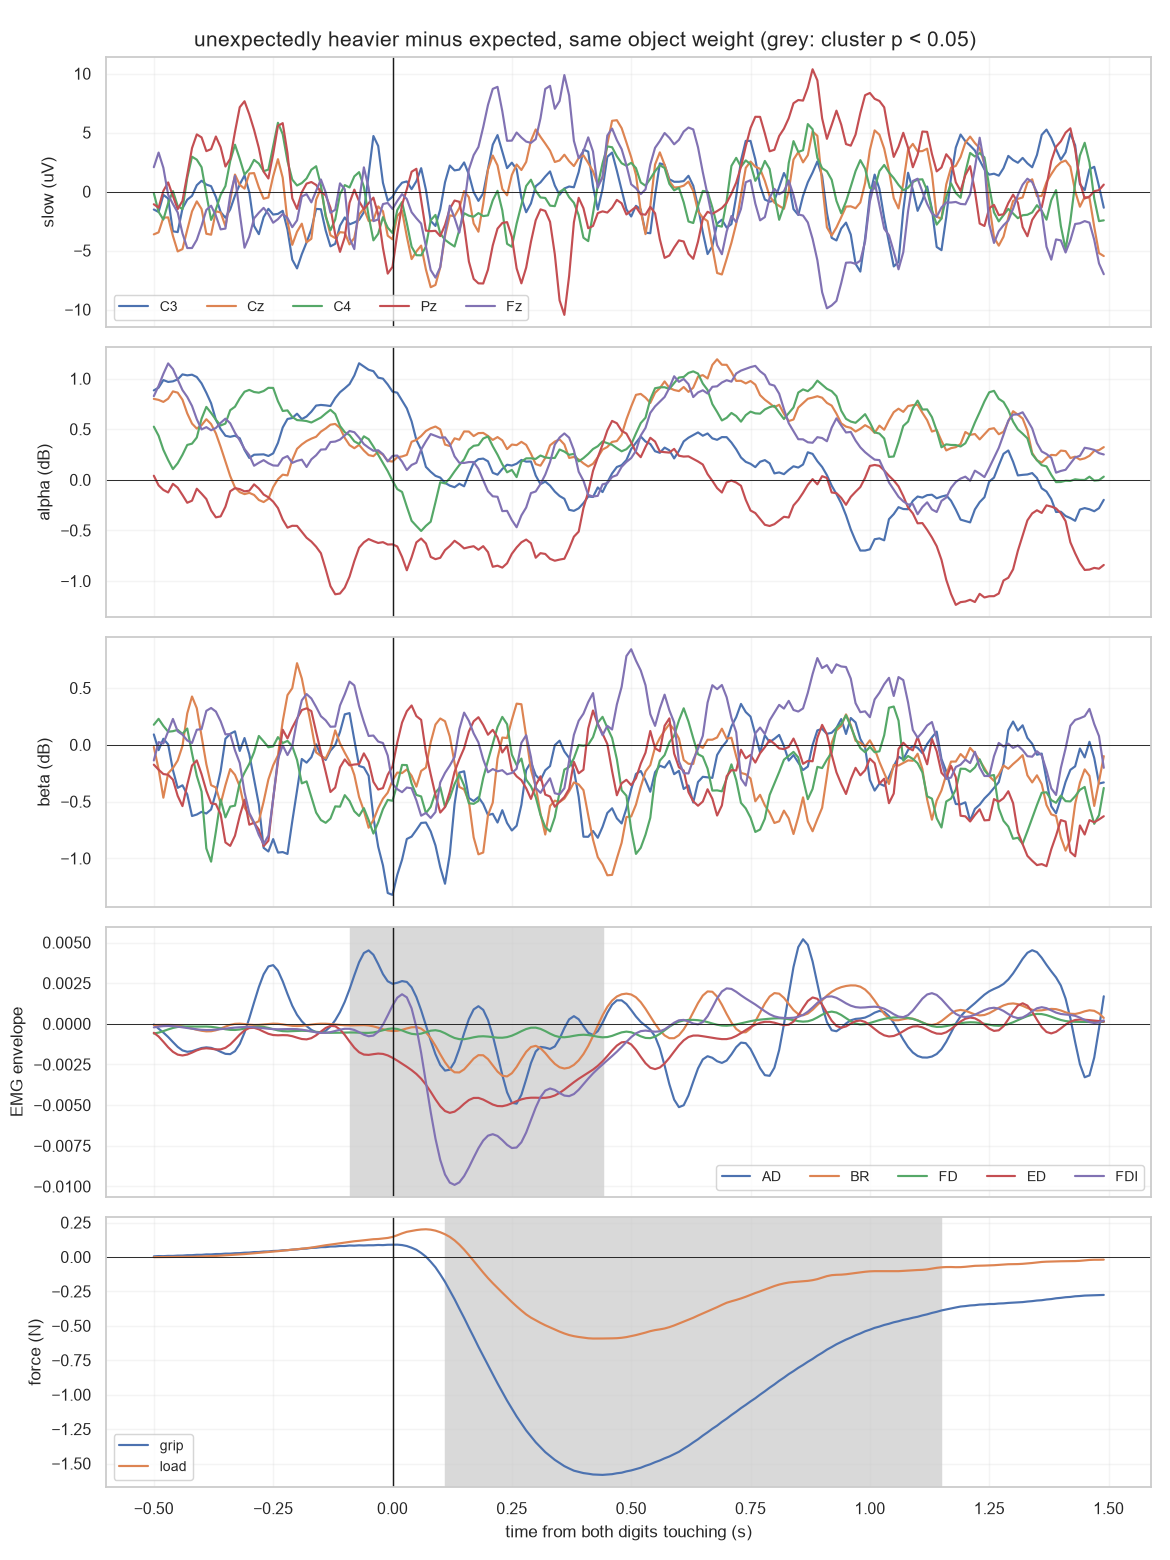
\includegraphics[height=68mm,width=\linewidth,keepaspectratio]{pe_error_heavier.png}}
    \column{0.52\linewidth}
    \centering\scriptsize
    \begin{tabular}{llcc}
      \toprule
      & signal & first cluster & best $p$ \\
      \midrule
      heavier & slow EEG & --- & 0.071 \\
      & alpha & 450 ms & 0.028 \\
      & beta & --- & 0.25 \\
      & EMG (ED) & $-90$ ms & 0.002 \\
      & force & 110 ms & 0.001 \\
      \midrule
      lighter & slow EEG & 210 ms & 0.003 \\
      & alpha & 720 ms & 0.044 \\
      & beta & 420 ms & 0.040 \\
      & EMG & --- & 0.11 \\
      & force & 710 ms & 0.007 \\
      \bottomrule
    \end{tabular}
    \raggedright
    \begin{itemize}\scriptsize
      \item Heavier: only alpha rises (450--810 ms), over a wide area that includes Fp1 and Fp2.
      \item EMG differs 90 ms \emph{before} touch: the expectation is visible in the muscles.
      \item 10 uncorrected cluster tests; with Bonferroni over the 6 EEG tests only the lighter positive wave survives.
    \end{itemize}
  \end{columns}
\end{frame}

\begin{frame}{Pilot 2: what we expected, and what we got}
  \centering\scriptsize
  \renewcommand{\arraystretch}{1.2}
  \begin{tabular}{@{}>{\raggedright}p{14mm}>{\raggedright}p{46mm}>{\raggedright\arraybackslash}p{70mm}@{}}
    \toprule
    & expected (from the physics and the literature) & what we got (touch at 0 s, cluster $p<0.05$) \\
    \midrule
    \textbf{heavier} & Grip is planned for a lighter object, so the object does not lift when expected; force must
      be raised mid-lift. Body: lower grip early, longer load phase. EEG: a response when the expected lift-off fails
      (about 200--400 ms after touch). &
      Body: EMG of ED lower from $-90$ ms (before touch); grip force lower from 110 ms for over a second; load phase
      181 ms longer. EEG: \textbf{no} slow or beta cluster (best $p$ 0.071 and 0.25); only alpha rises at 450--810 ms
      over a wide area that includes Fp1/Fp2. \\
    \midrule
    \textbf{lighter} & Grip is planned for a heavier object, so the object jumps up early. Body: brief force overshoot,
      shorter load phase. EEG: a response to the unexpected early lift-off. &
      Body: grip and load higher at 60--360 ms (only $p\approx0.06$), grip lower from 710 ms ($p$ 0.007); no EMG
      cluster. EEG: negative wave 210--390 ms and positive wave 560--800 ms over C3, Cz, CP1, Pz ($p$ 0.027 and
      0.003); beta drop from 420 ms. \\
    \bottomrule
  \end{tabular}
  \begin{tcolorbox}[notebox,title={In short}]
    \scriptsize The body responds in both conditions. The EEG responds clearly only when the object is lighter, and
    even then after the force has started to differ.
  \end{tcolorbox}
\end{frame}

\begin{frame}{Pilot 2: why heavier and lighter give different clusters}
  \begin{columns}[T]
    \column{0.50\linewidth}
    \begin{tcolorbox}[stagebox,title={Why the body clusters differ}]
      \scriptsize
      \begin{itemize}
        \item A cluster needs a difference that is \emph{consistent} across the 12 participants and lasts long enough.
        \item \textbf{Heavier}: the planned force is too low for the whole load phase, which is 181 ms longer. That is
              a large, long and same-signed difference, so force and EMG form strong clusters. ED is already lower
              before touch: the hand is pre-shaped for a lighter object.
        \item \textbf{Lighter}: a light object needs little force, so the overshoot is small and brief and is
              corrected within a few hundred ms. Only the late grip reduction (scaling down to the light object) is
              long enough to be significant.
      \end{itemize}
    \end{tcolorbox}
    \column{0.46\linewidth}
    \begin{tcolorbox}[stagebox,title={Why the EEG clusters differ}]
      \scriptsize
      \begin{itemize}
        \item \textbf{Lighter}: the error is a sharp sensory \emph{event} (early lift-off, sudden acceleration),
              locked in time to touch and to lift-off, so an evoked response survives averaging. Its shape (negative,
              then a centro-parietal positive wave) fits an evoked response to a surprising event.
        \item \textbf{Heavier}: the error is an \emph{absence} (lift-off does not come). There is no sharp sensory
              transient, and the moment of the error varies, so an evoked response would be weak or smeared.
        \item Test of the smearing idea: realigning to lift-off (next slide) still gives no heavier EEG cluster.
      \end{itemize}
    \end{tcolorbox}
    {\scriptsize These are interpretations, not tested causes, except the realignment.\par}
  \end{columns}
\end{frame}

\begin{frame}{Pilot 2: is the cluster test working? Four checks}
  \begin{columns}[T]
    \column{0.49\linewidth}
    \textbf{1. False positives} (labels shuffled within participant and weight, 40 runs each)

    \smallskip
    \centering\scriptsize
    \begin{tabular}{lcc}
      \toprule
      & slow EEG & beta \\
      \midrule
      heavier & 0 / 40 & 3 / 40 \\
      lighter & 1 / 40 & 0 / 40 \\
      \bottomrule
    \end{tabular}
    \raggedright

    {\scriptsize 4 of 160 runs (2.5\%) give a cluster: the test holds its 5\% error rate, slightly conservative. The
    real clusters are not what the test produces by chance.\par}

    \medskip
    \textbf{2. Power} (an effect planted into shuffled data: 6 central-left channels, peak 300 ms, SD 50 ms; 8 runs each)

    \smallskip
    \centering\scriptsize
    \begin{tabular}{lccc}
      \toprule
      slow EEG & 3 $\mu$V & 6 $\mu$V & 10 $\mu$V \\
      \midrule
      heavier / lighter detected & 0 / 0 & 38 / 25\% & 100 / 100\% \\
      \midrule
      beta & 0.5 dB & 1 dB & 2 dB \\
      \midrule
      heavier / lighter detected & 0 / 0 & 13 / 38\% & 100 / 100\% \\
      \bottomrule
    \end{tabular}
    \column{0.47\linewidth}
    \textbf{3. Threshold-free (TFCE)}, touch-aligned
    \begin{itemize}\scriptsize
      \item heavier: slow none (min $p$ 0.055), beta none, alpha from 500 ms ($p$ 0.015)
      \item lighter: slow from 110 ms ($p$ 0.005), beta from 460 ms ($p$ 0.015), alpha none
    \end{itemize}
    \textbf{4. Realigned to lift-off}
    \begin{itemize}\scriptsize
      \item heavier: still no EEG cluster ($p<0.1$) in slow, alpha or beta; force and EMG clusters remain
      \item lighter: slow EEG from lift-off to 580 ms ($p$ 0.005), but grip and load already differ
            400--50 ms \emph{before} lift-off ($p$ 0.045)
    \end{itemize}
    \begin{tcolorbox}[askbox,title={What ``no cluster'' means}]
      \scriptsize With 12 participants the test reliably finds an effect of about 10 $\mu$V or 2 dB (about 1.4--2
      between-participant SD) and misses one of 3 $\mu$V or 0.5 dB. So the heavier result means: no EEG effect of
      that size; a smaller one cannot be excluded.
    \end{tcolorbox}
  \end{columns}
\end{frame}

\begin{frame}{Pilot 3 and 4: expectation before contact, and learning}
  \begin{columns}[T]
    \column{0.52\linewidth}
    \FigRow{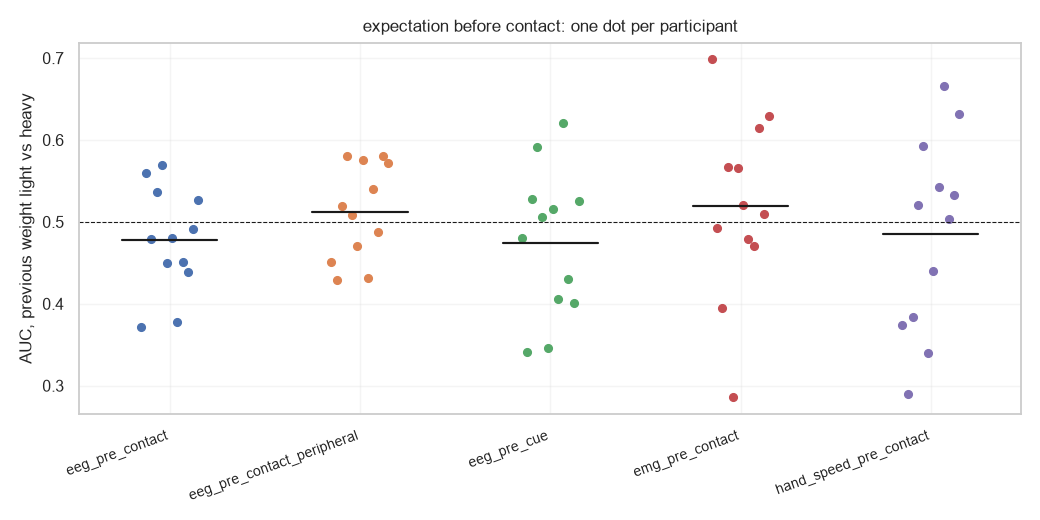
\includegraphics[width=\linewidth,height=29mm,keepaspectratio]{pe_expectation.png}}
    \FigCap{AUC of decoding the previous weight (165 vs 660 g) in the 0.6 s before contact; one dot per participant.}
    \centering\scriptsize
    \begin{tabular}{lcc}
      \toprule
      decoder input & mean AUC & $p$ \\
      \midrule
      central EEG, before contact & 0.478 & 0.83 \\
      peripheral EEG & 0.512 & 0.19 \\
      central EEG, before the LED & 0.474 & 0.79 \\
      EMG & 0.519 & 0.23 \\
      hand speed & 0.485 & 0.60 \\
      \bottomrule
    \end{tabular}
    \column{0.44\linewidth}
    \begin{tcolorbox}[notebox,title={3. Expectation: not decodable}]
      \scriptsize No decoder beats chance. The null of this decoder is itself slightly below 0.5 (about 0.47, a known
      bias of pooled-fold AUC), but the real AUC is not above it either.
    \end{tcolorbox}
    \begin{tcolorbox}[notebox,title={4. Learning (exploratory): no effect}]
      \scriptsize Partial Spearman between the beta response (0.2--0.6 s) and the size of the next lift's force update,
      controlling peak force, load-phase duration and EMG: Fisher $z$ $-0.063$, positive in 4 of 12, $p$ 0.18.
    \end{tcolorbox}
    \begin{tcolorbox}[askbox,title={Pilot verdict, and the question for the supervisor}]
      \scriptsize behaviour pass \quad error half \quad expectation fail \quad learning none\\
      $\Rightarrow$ no claim that is separate from the movement.\\[2pt]
      Can any analysis separate an EEG error signal from the response to the corrective movement in this data, or
      does that need a perturbation design?
    \end{tcolorbox}
  \end{columns}
\end{frame}

%% =============================================================
\section{Decisions}
%% =============================================================

\begin{frame}{Main question 2: how could the current goal continue?}
  \begin{columns}[T]
    \column{0.48\linewidth}
    \begin{tcolorbox}[stagebox,title={Option A: causal direction}]
      \scriptsize
      Test whether EEG \emph{leads} EMG: lead--lag, Granger causality or transfer entropy, corticomuscular coherence
      with direction.\\[2pt]
      \textbf{For:} a direction claim does not need a large accuracy gain.\\
      \textbf{Against:} the same task clock drives both signals; any lead can come from the shared LED and event
      times unless they are regressed out first. Our causal horizons (0--1000 ms) already found no gain beyond B.
    \end{tcolorbox}
    \column{0.48\linewidth}
    \begin{tcolorbox}[stagebox,title={Option B: interpretability}]
      \scriptsize
      Explain what the EEG part of the model uses (electrodes, bands, time).\\[2pt]
      \textbf{Problem:} interpretation is only as meaningful as the effect it explains. E keeps 90\% with another
      trial's EEG, so its maps mostly show the \emph{task-locked} pattern (beta ERD at C3/CP1 when the hand moves),
      which is known. F's EEG gain is about zero, so there is nothing to explain in F.\\[2pt]
      \textbf{What could still be valid:} interpret only the trial-specific part (E minus phase-swapped E), with the
      timing model as the reference.
    \end{tcolorbox}
  \end{columns}
  \Verify{\scriptsize Which of A or B do you see as publishable with these results? Is interpreting the trial-specific 10\% meaningful when it adds nothing over the timing model?}
\end{frame}

\begin{frame}{Main question 3: change the goal to an audit?}
  \begin{columns}[T]
    \column{0.50\linewidth}
    {\footnotesize\textbf{What an audit is.} Re-run published EEG decoders on WAY-EEG-GAL with their own protocol, then add the
    controls they did not report:\par}
    \begin{enumerate}\scriptsize
      \item a causal task-timing baseline (no brain at all)
      \item EEG of another trial with events aligned (phase\_swap)
      \item peripheral-channel band power (eye, neck)
      \item series-held-out instead of random-window splits
    \end{enumerate}
    {\scriptsize If the timing model or swapped EEG reaches the same accuracy, the reported decoding is task timing.
    Our own v3 controls are already this protocol: E keeps 90\% of its accuracy with another trial's EEG.\par}
    \column{0.46\linewidth}
    \begin{tcolorbox}[notebox,title={Targets on this dataset (no timing control in their abstracts)}]
      \scriptsize
      \begin{itemize}
        \item Amiri \& Shalchyan 2025 (CMPB): EMG envelope from EEG band envelopes, CNN-LSTM
        \item Dangi \& Meena 2025, 2026: grasp force $R^2\approx0.8$; several movement parameters
        \item Kaggle GAL detection (2015): very high AUC, artifact doubts in its own forum
      \end{itemize}
      Precedent: Antelis et al.\ 2013, EEG kinematics decoding at chance once tested properly.
    \end{tcolorbox}
    \begin{tcolorbox}[notebox,title={Risks}]
      \scriptsize Exact re-implementation is needed; full texts not yet read. If their results survive the controls,
      the paper turns into a positive replication (still reportable). Venue: J.\ Neural Eng.\ or Imaging Neuroscience.
    \end{tcolorbox}
  \end{columns}
  \Verify{\scriptsize Is an audit / negative-result paper a good outcome for this project? Should we contact the original authors for their code first?}
\end{frame}

\begin{frame}{Other questions for the supervisor}
  \begin{columns}[T]
    \column{0.48\linewidth}
    \textbf{Method}
    \begin{enumerate}\scriptsize
      \item Is $r$ on smooth envelopes misleading (Antelis 2013)? Should MSE skill be the headline metric everywhere?
      \item Task events are detected from the force recording; is that a leak in favour of B?
      \item Do we need the artifact trainings (central, peripheral, eye-regressed EEG) before any claim, given that the
            result is negative?
      \item Is 12 participants enough for the group tests, or should we add a second dataset?
    \end{enumerate}
    \column{0.48\linewidth}
    \textbf{Direction}
    \begin{enumerate}\scriptsize\setcounter{enumi}{4}
      \item One audit paper with the v3 controls and the pilot as a supplement, or two separate papers?
      \item If the audit is chosen: how many published methods must be re-implemented to be convincing?
      \item Should the v1--v3 models appear in the paper, or only the controls and the timing baselines?
      \item Timeline and target date for a first draft?
    \end{enumerate}
  \end{columns}
\end{frame}

\begin{frame}{Summary}
  \begin{enumerate}\small
    \item v1 and v2 predict EMG well (up to $r$ 0.87), but the accuracy comes from kinematics.
    \item EEG alone reaches $r$ 0.63--0.65, yet a model that only knows the task timing reaches 0.81.
    \item v3: with past movement and past events known, EEG adds nothing at any horizon from 0 to 1000 ms.
    \item The kinematic guide does not improve the EEG-only model; that model keeps 90\% of its accuracy with
          another trial's EEG.
    \item The prediction-error pilot finds an EEG response, but only after the movement differs.
  \end{enumerate}
  \begin{tcolorbox}[askbox,title={Decision needed}]
    \small Keep the goal (causal direction or interpretability), or turn the project into an audit of EEG decoding on
    WAY-EEG-GAL?
  \end{tcolorbox}
\end{frame}

\begin{frame}[standout]
  \centering
  \Large Thank you\\[10pt]
  \normalsize Questions?
\end{frame}

%% =============================================================
\appendix
\metroset{sectionpage=simple}
\section{Appendix}
%% =============================================================

\begin{frame}{Appendix: causal timing baselines (v3, step 2)}
  \centering\small
  \begin{tabular}{lcccc}
    \toprule
    model & 0 ms & 200 ms & 500 ms & 1000 ms \\
    \midrule
    cue (sees the future, ceiling) & 0.576 & --- & --- & --- \\
    phase (sees the future, ceiling) & 0.814 & --- & --- & --- \\
    causal\_cue & 0.539 & 0.558 & 0.588 & 0.619 \\
    events\_causal & 0.764 & 0.761 & 0.753 & 0.729 \\
    \bottomrule
  \end{tabular}
  \FigCap{Mean $r$ over 12 participants. Even the causal past-events model beats the EEG-only model (0.63).}
\end{frame}

\begin{frame}{Appendix: v2 triptychs, P3}
  \begin{columns}[T]
    \column{0.49\linewidth}
    \FigRow{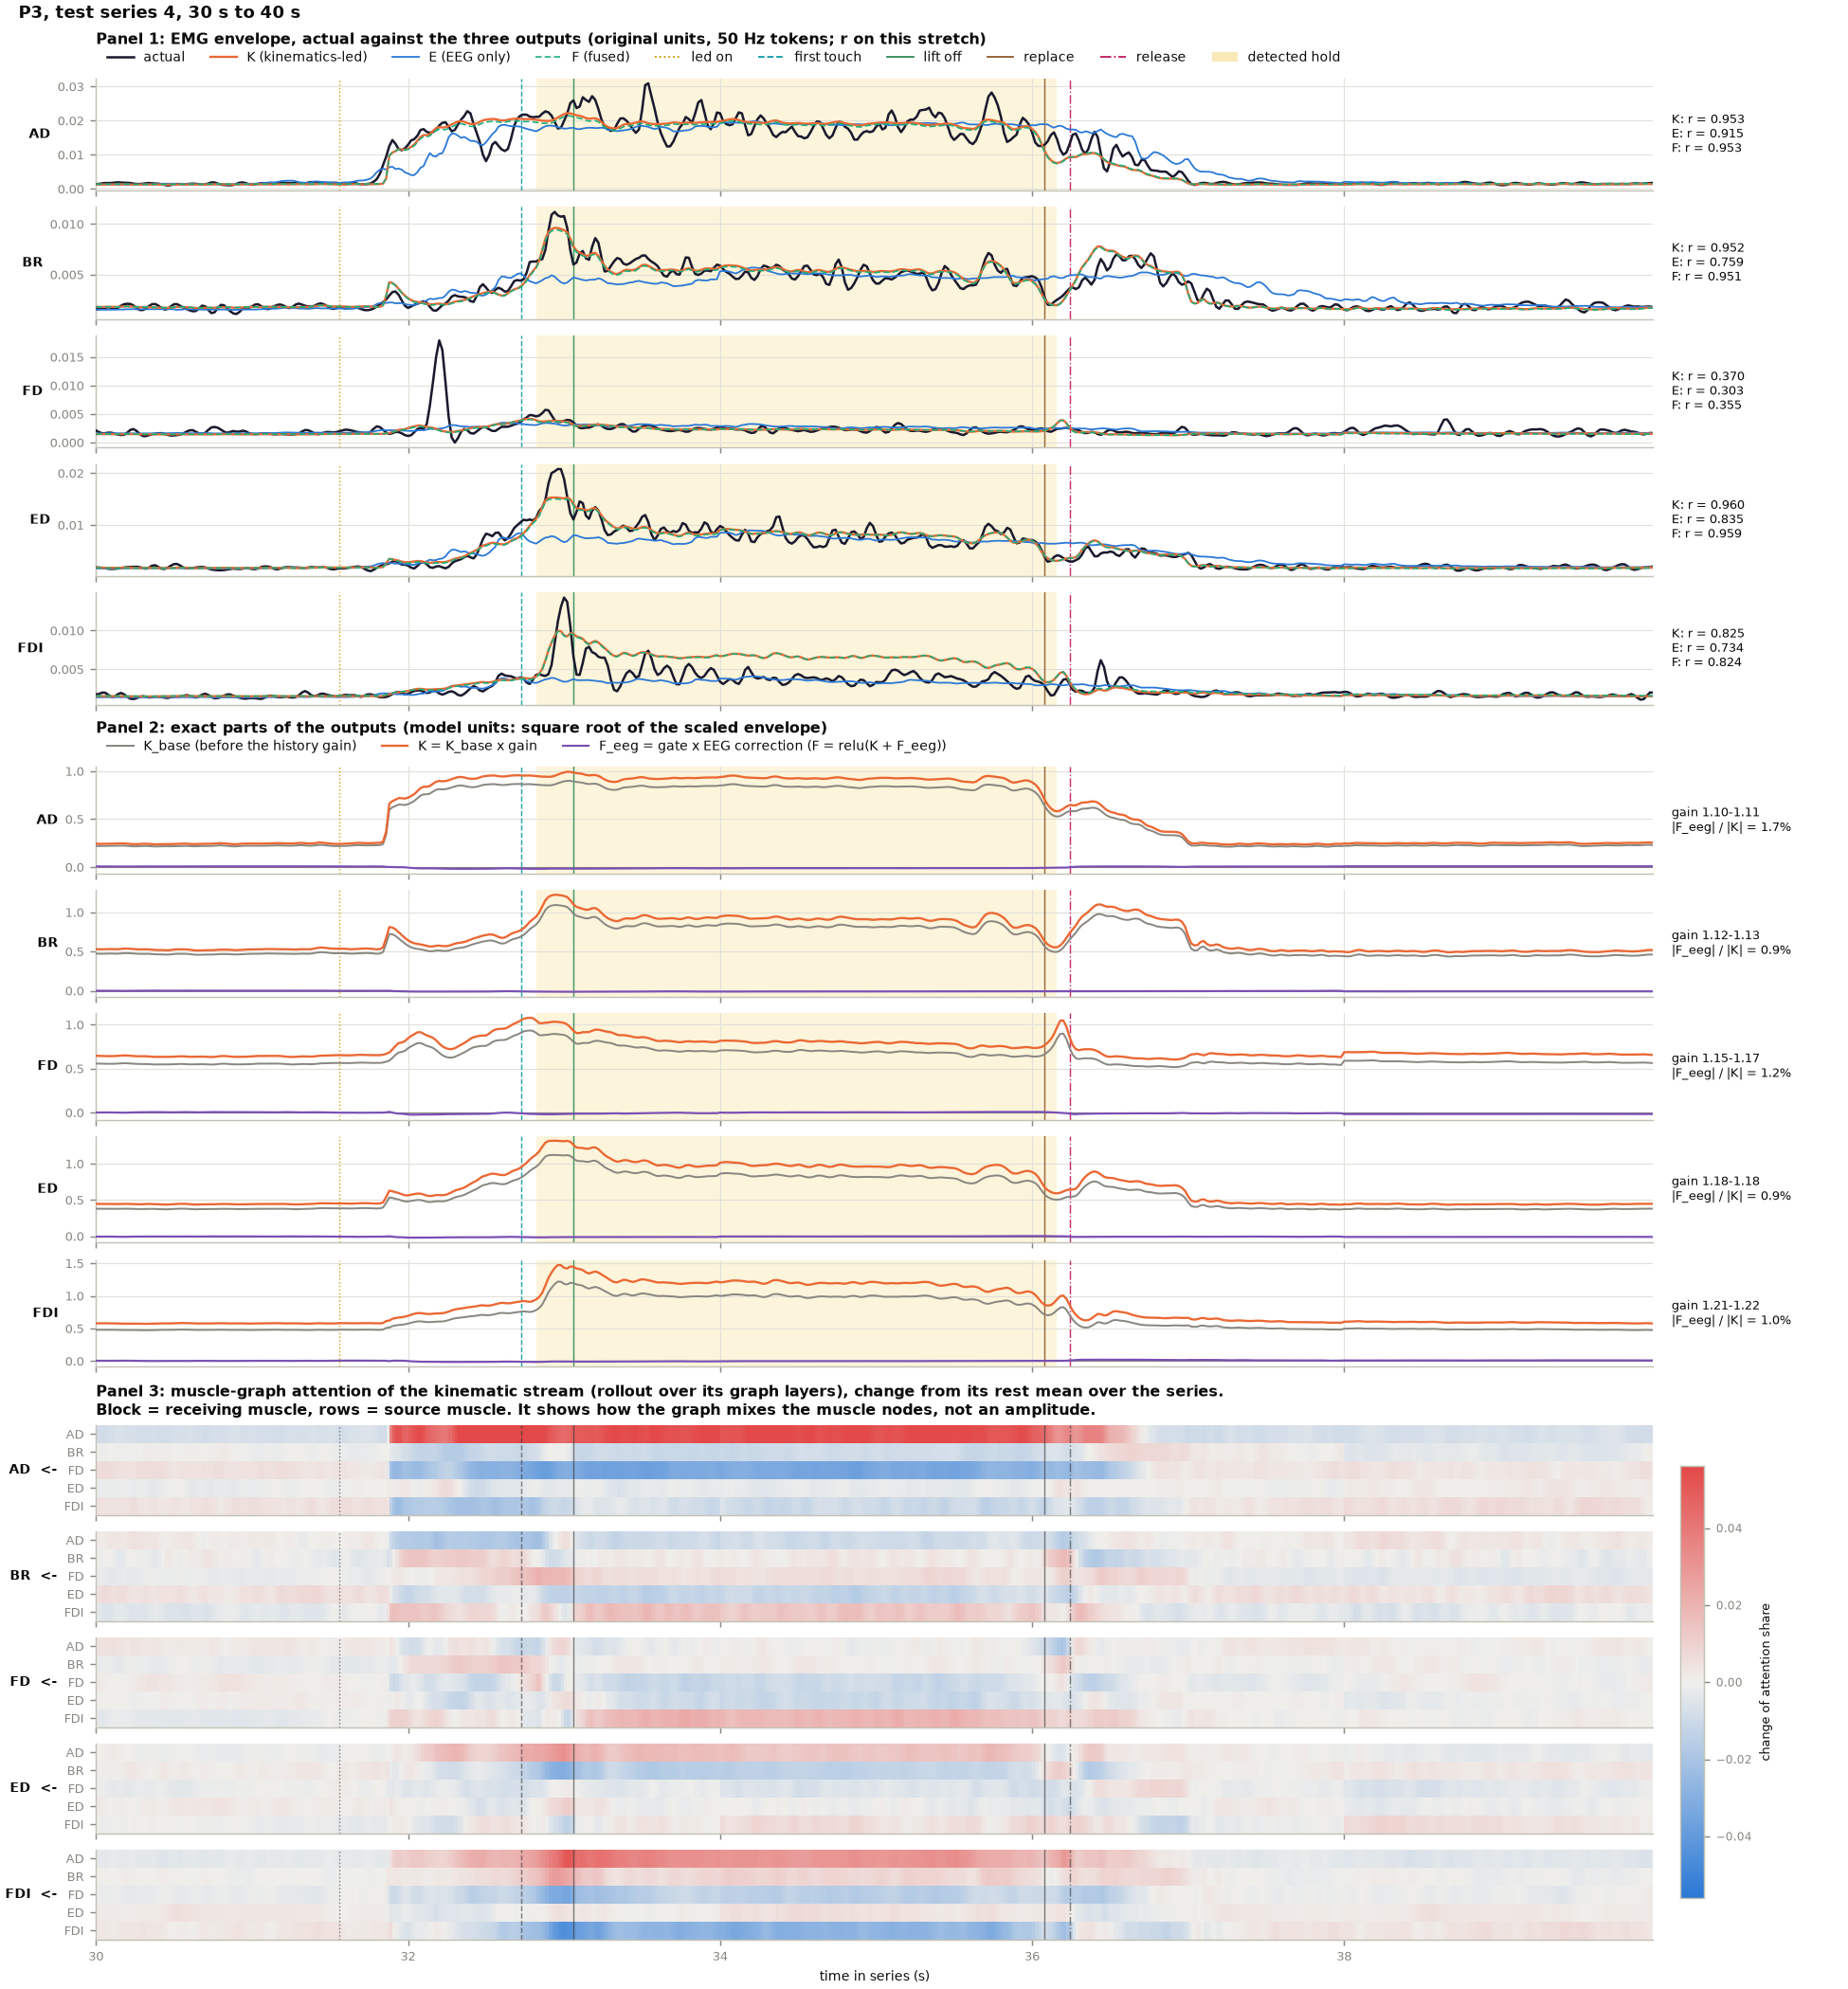
\includegraphics[height=66mm,width=\linewidth,keepaspectratio]{trip_P3_S04.png}}
    \FigCap{P3, test series 4.}
    \column{0.49\linewidth}
    \FigRow{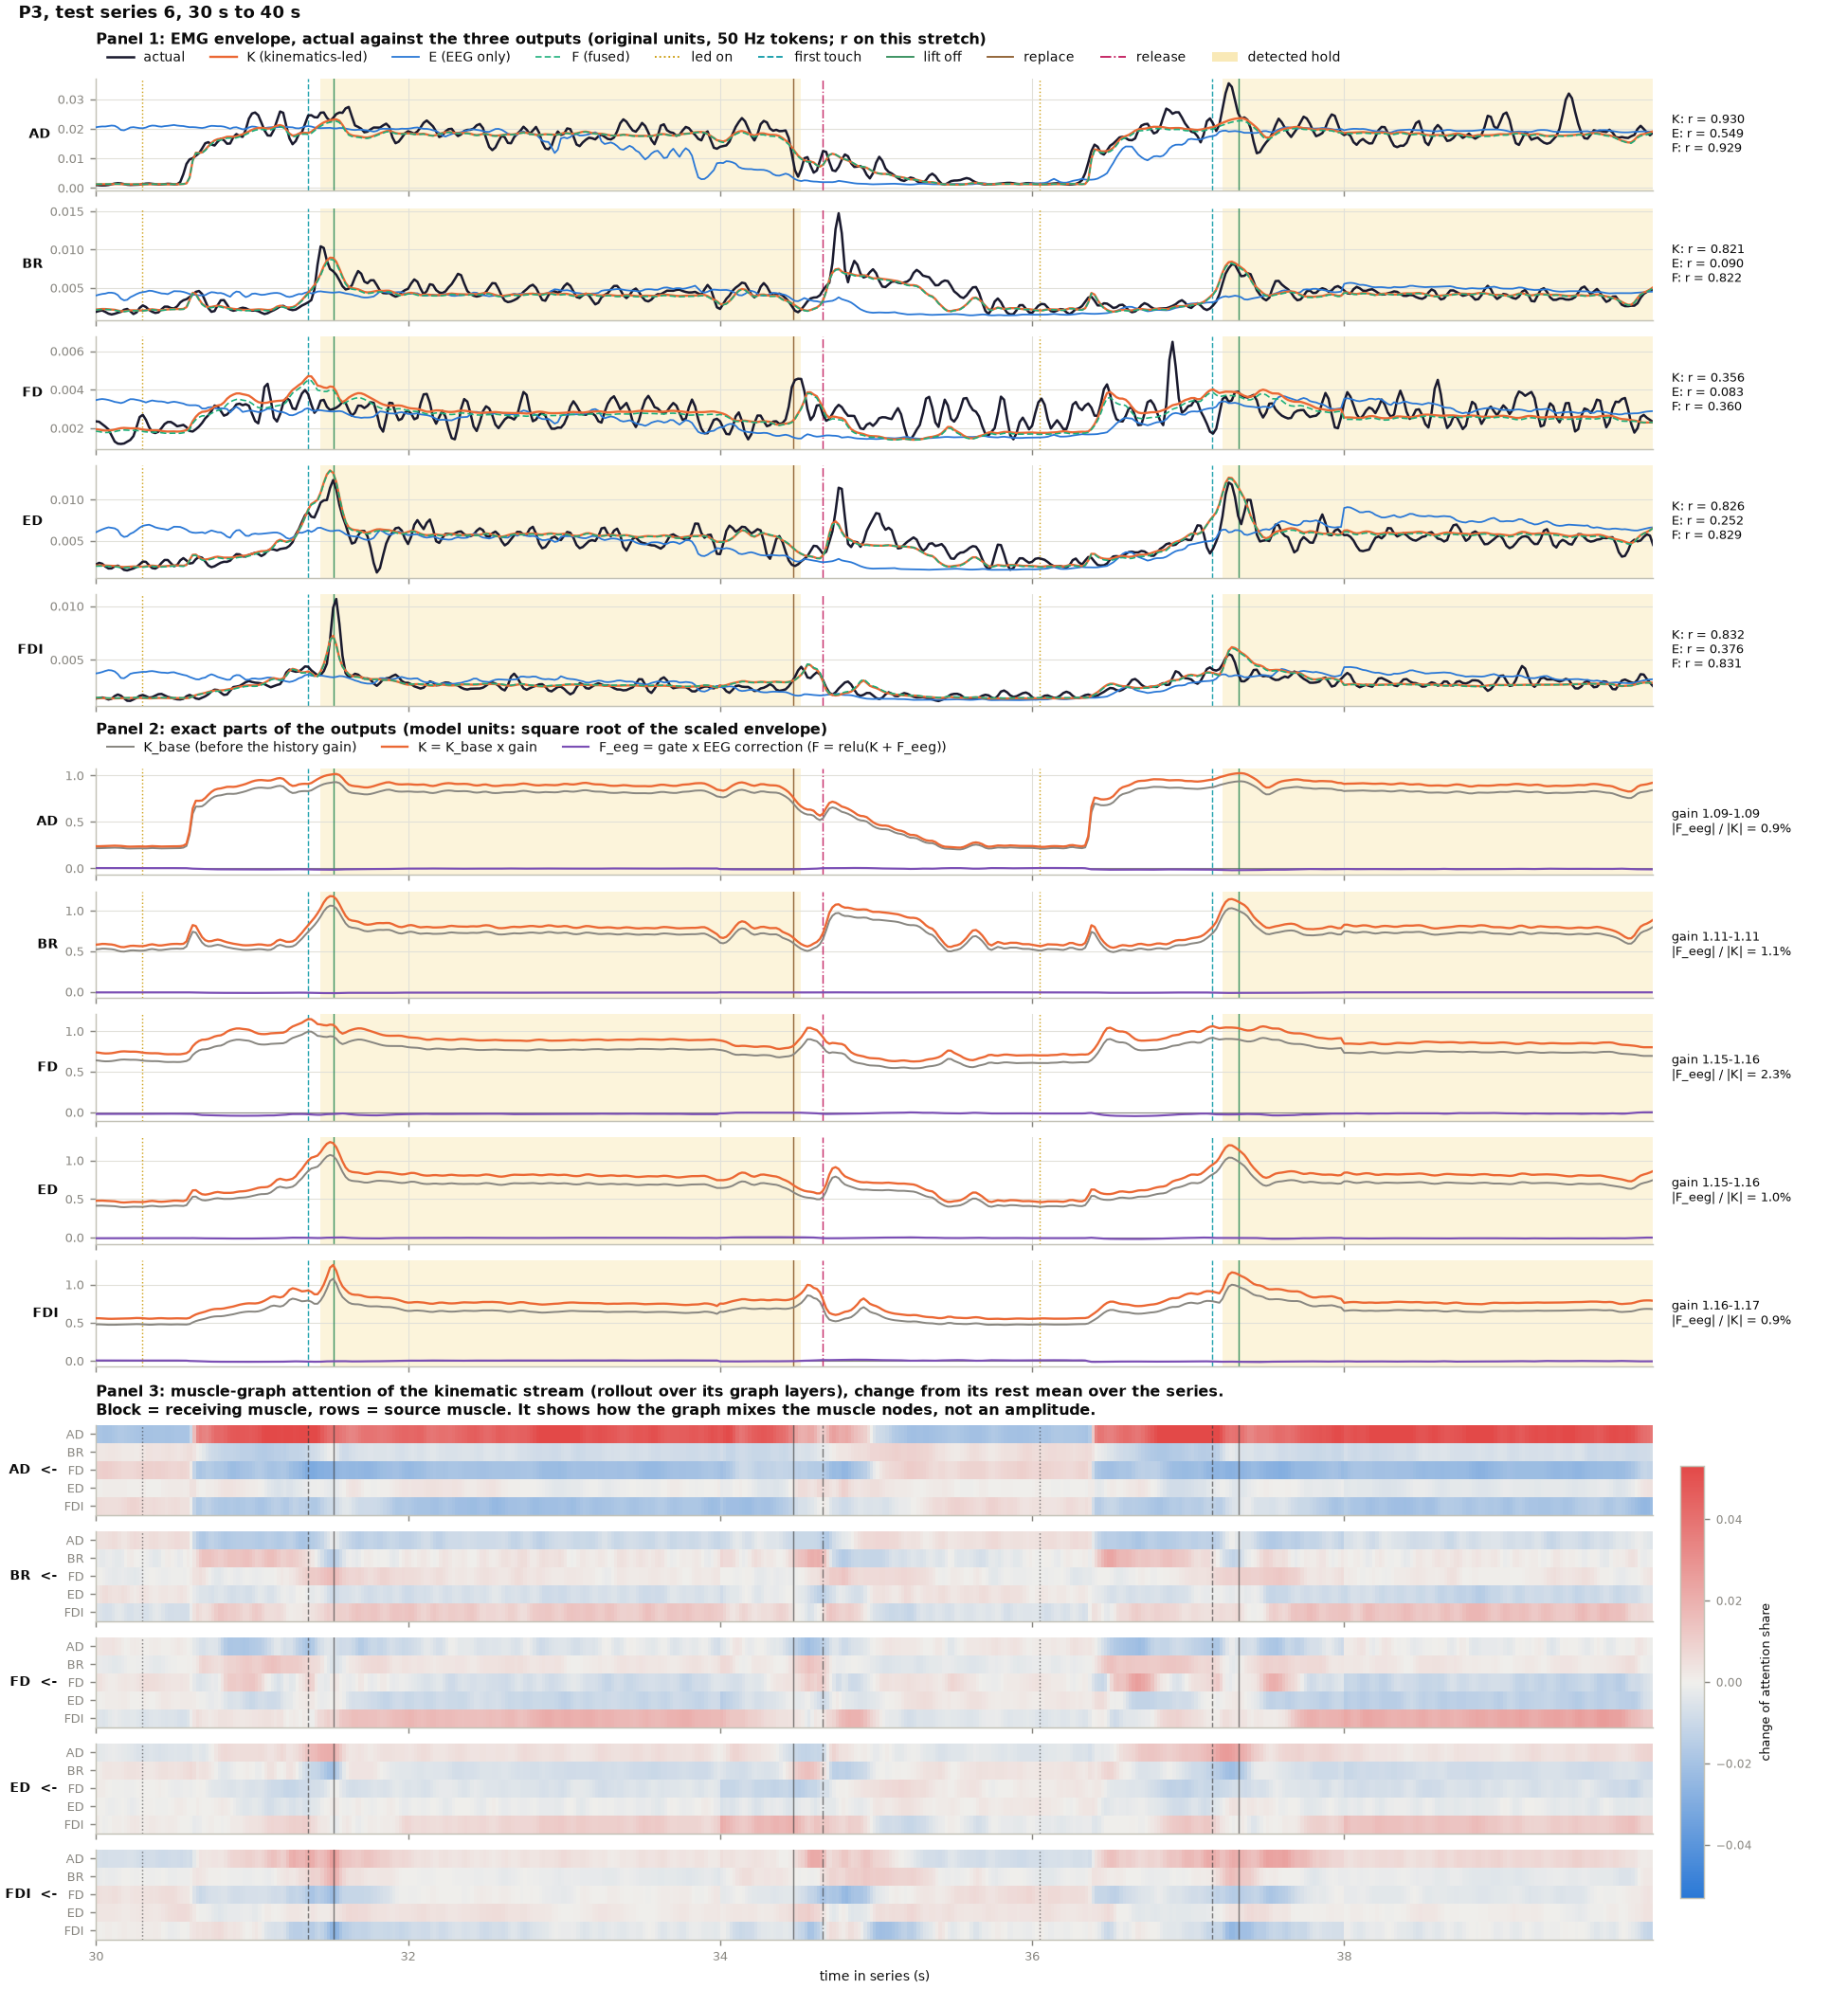
\includegraphics[height=66mm,width=\linewidth,keepaspectratio]{trip_P3_S06.png}}
    \FigCap{P3, test series 6.}
  \end{columns}
\end{frame}

\begin{frame}{Appendix: v2 triptychs, P2 and P4}
  \begin{columns}[T]
    \column{0.49\linewidth}
    \FigRow{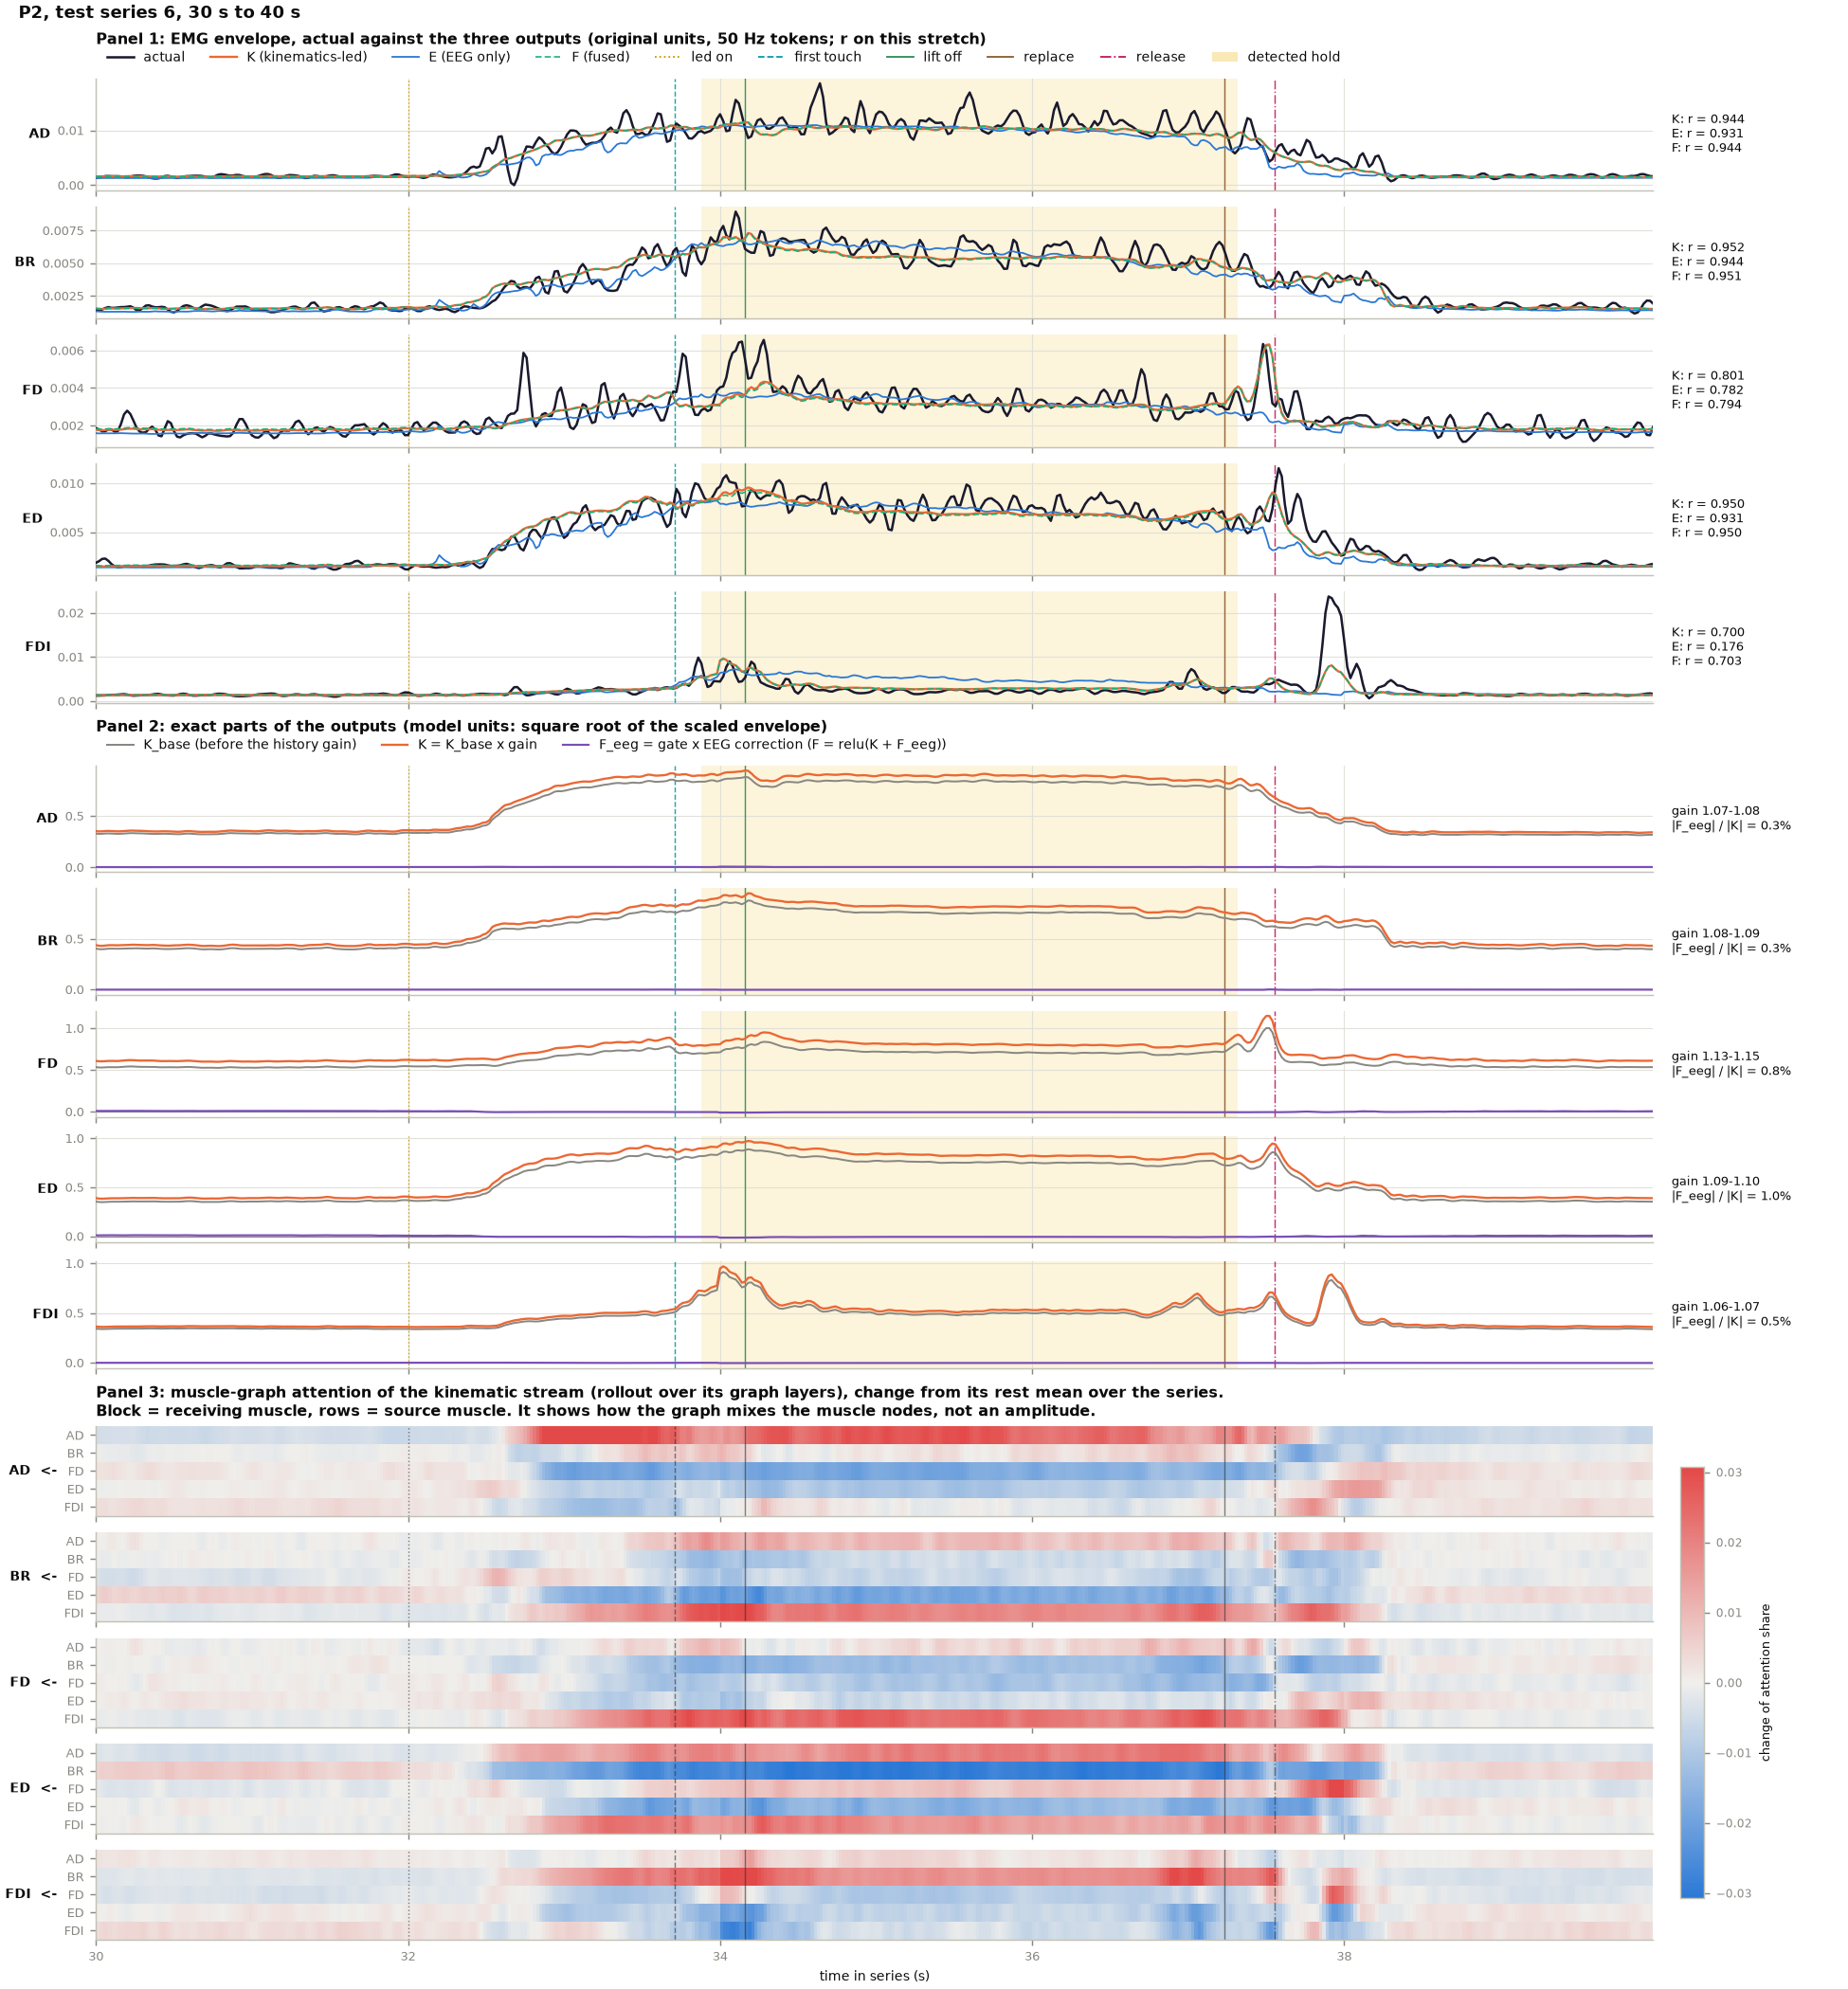
\includegraphics[height=66mm,width=\linewidth,keepaspectratio]{trip_P2_S06.png}}
    \FigCap{P2, test series 6.}
    \column{0.49\linewidth}
    \FigRow{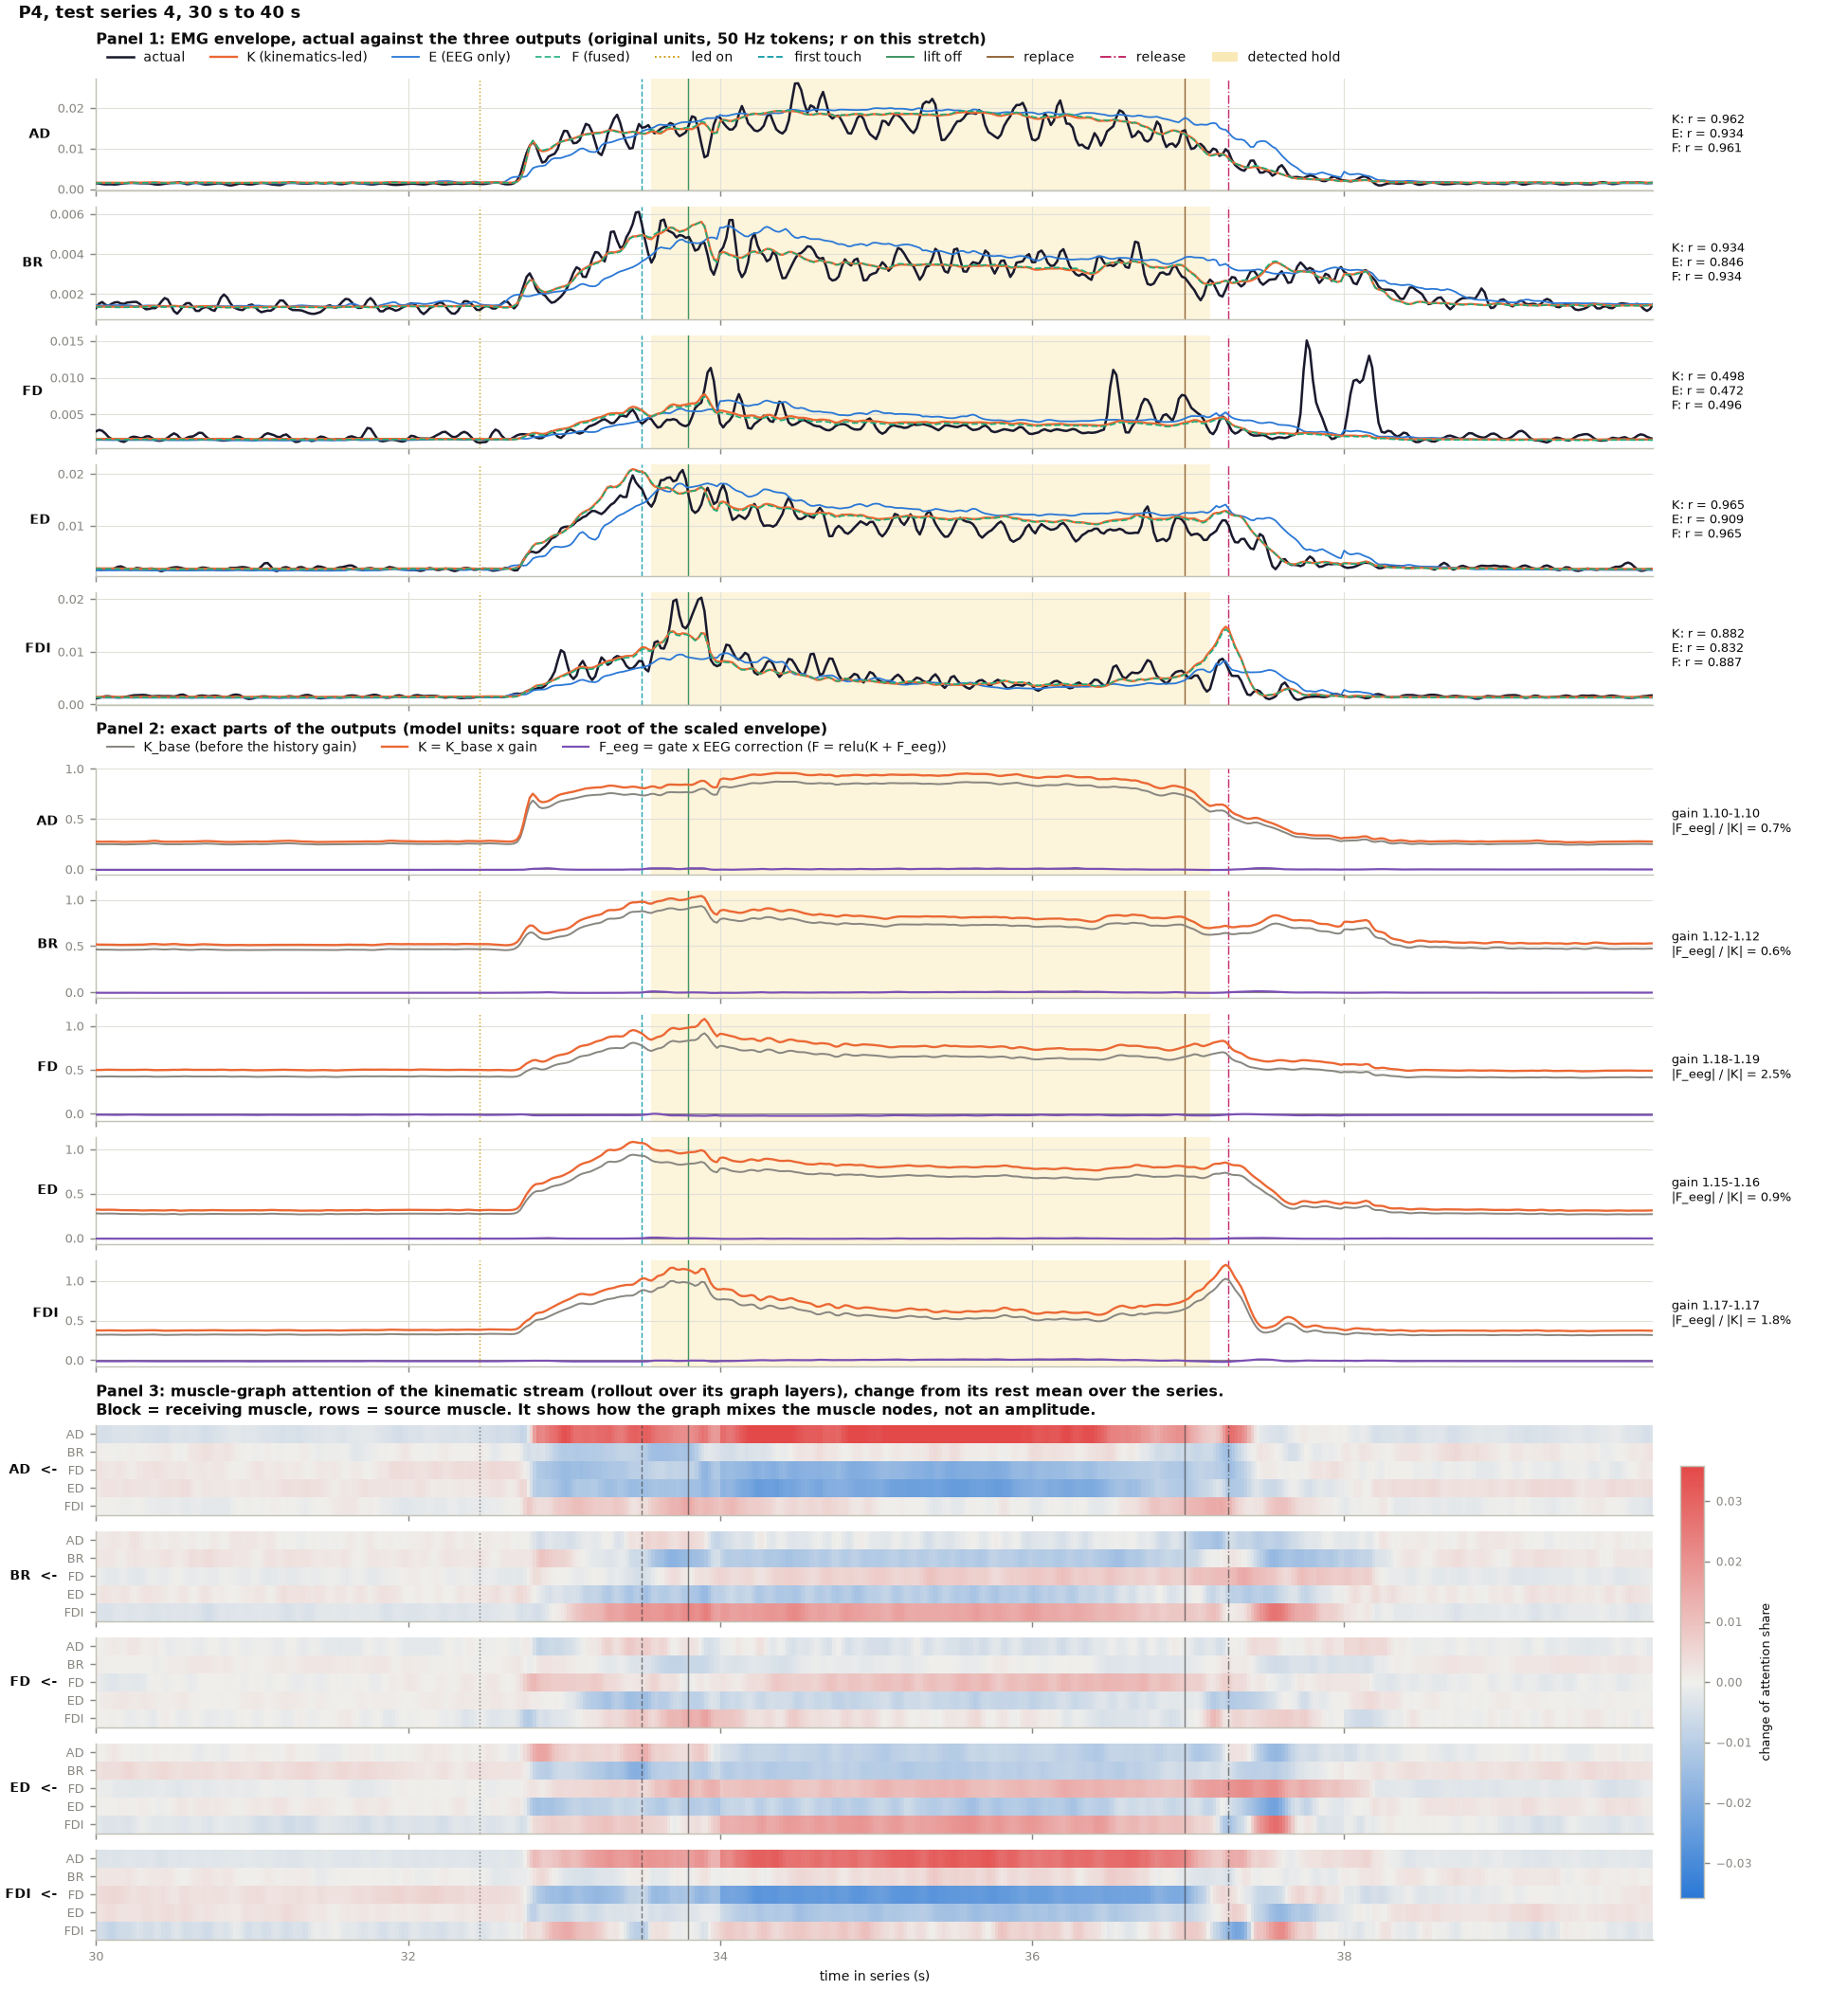
\includegraphics[height=66mm,width=\linewidth,keepaspectratio]{trip_P4_S04.png}}
    \FigCap{P4, test series 4.}
  \end{columns}
\end{frame}

\begin{frame}{Appendix: interpretability, P2}
  \FigRow{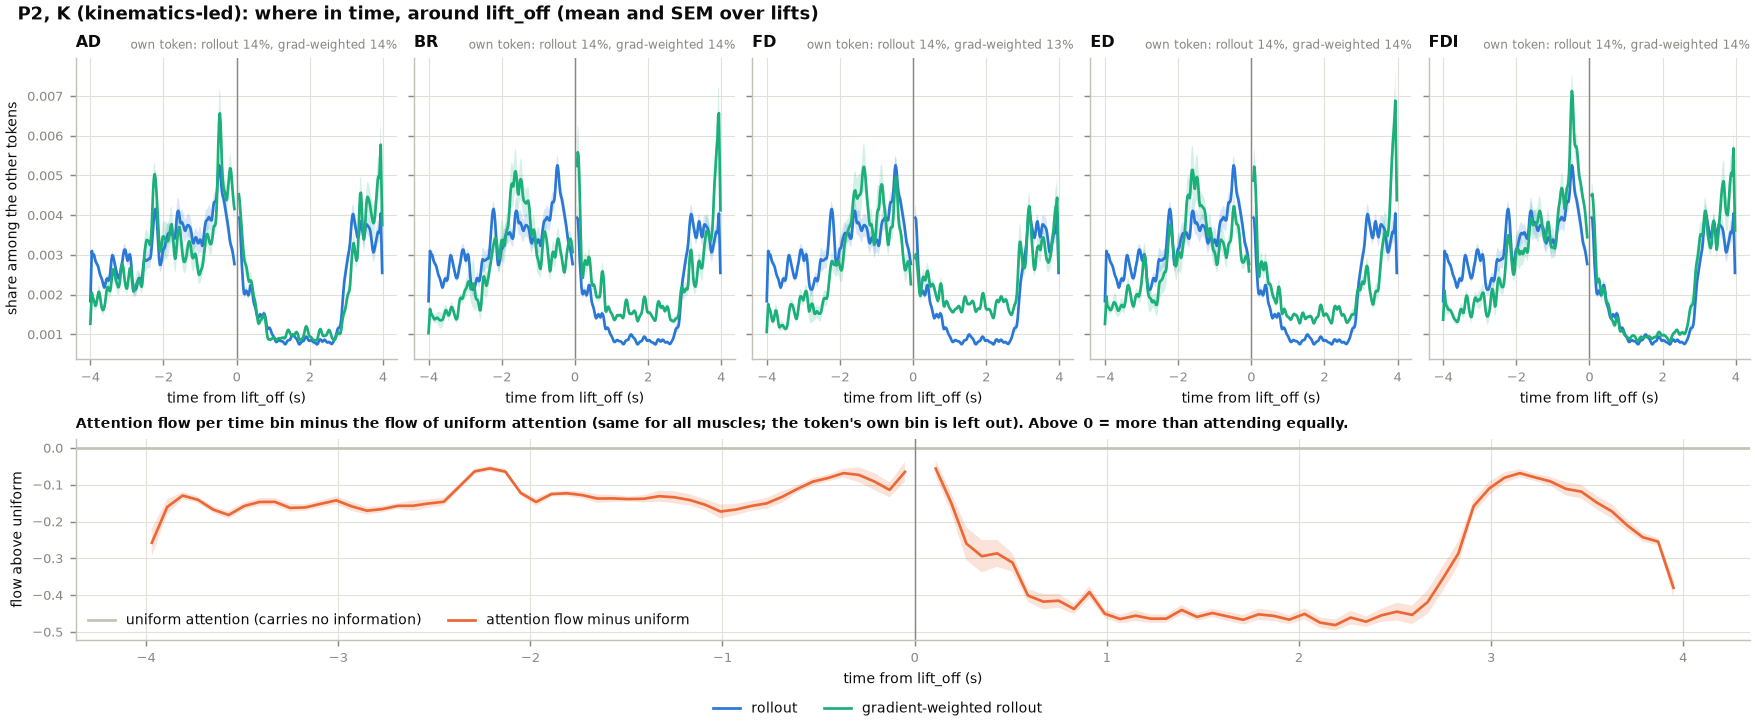
\includegraphics[width=0.49\textwidth,height=21mm,keepaspectratio]{P2_time_K_lift_off.png}\hspace{2mm}%
          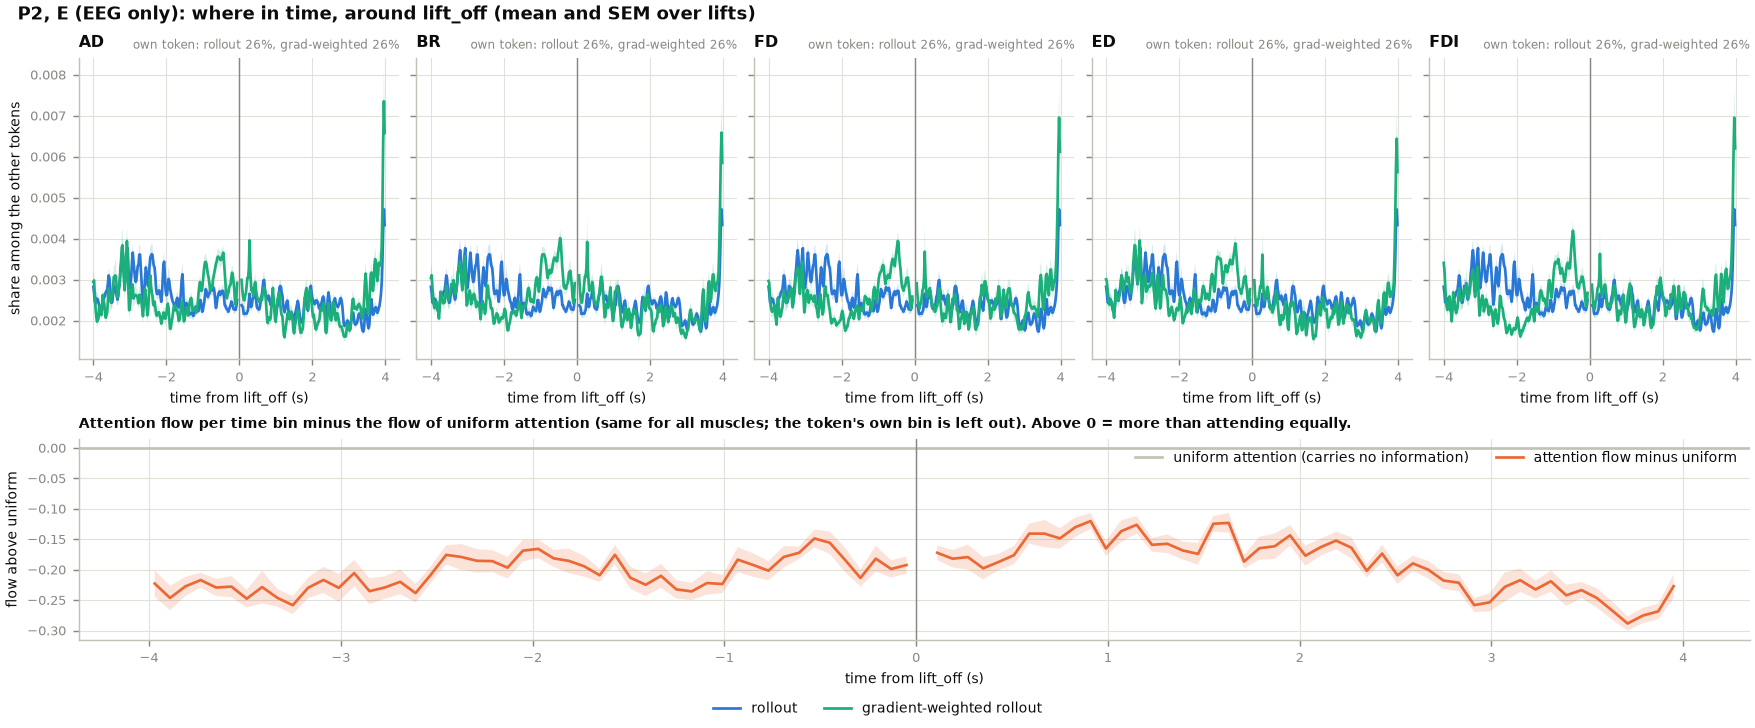
\includegraphics[width=0.49\textwidth,height=21mm,keepaspectratio]{P2_time_E_lift_off.png}}
  \FigCap{Time share around lift-off. Left: K, the same pattern as P1. Right: E, almost flat.}
  \vspace{1mm}
  \FigRow{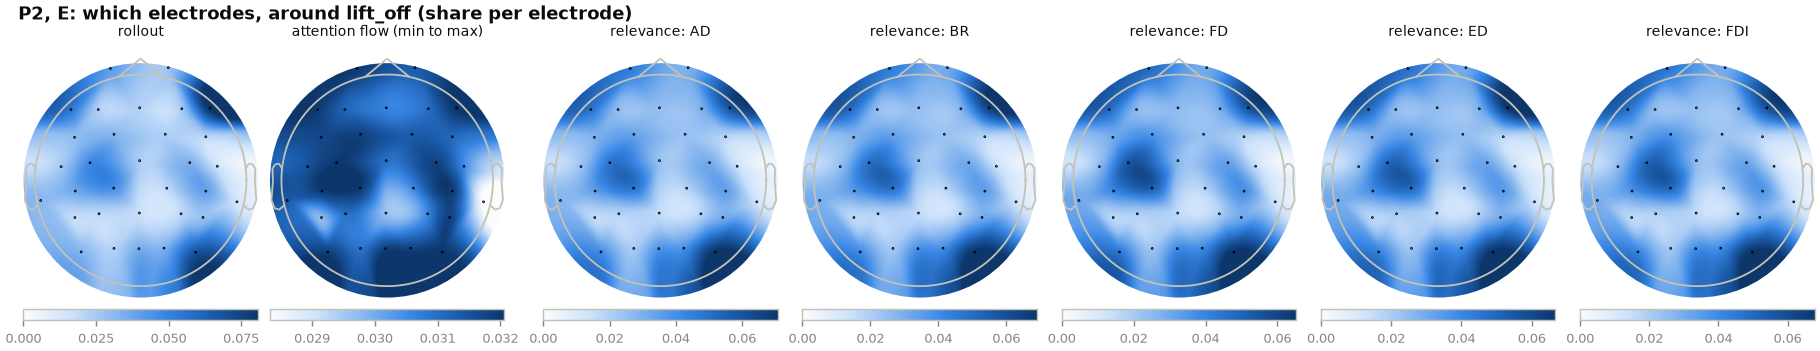
\includegraphics[width=\textwidth,height=16mm,keepaspectratio]{P2_scalp_E_lift_off.png}}
  \FigCap{E electrode share: weaker left central focus, more weight on the edges of the head.}
  \vspace{1mm}
  \FigRow{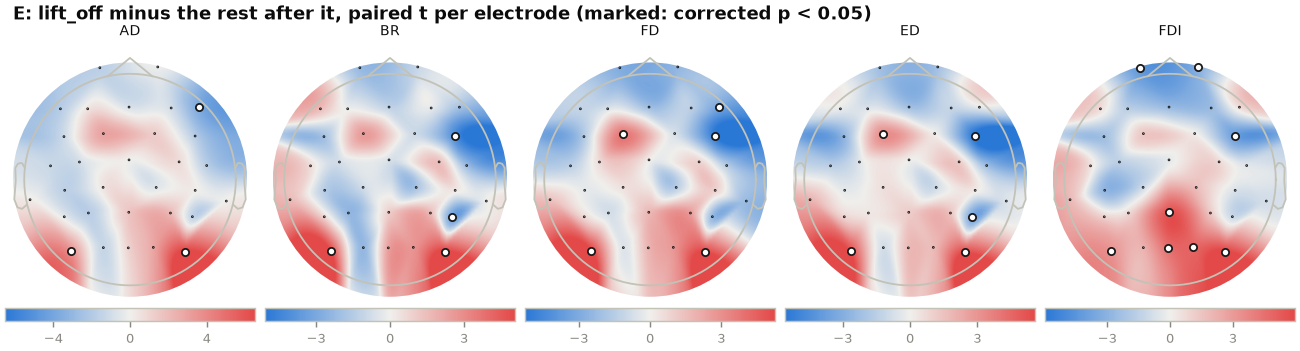
\includegraphics[width=0.48\textwidth,height=17mm,keepaspectratio]{P2_rest_contrast_lift_off.png}\hspace{2mm}%
          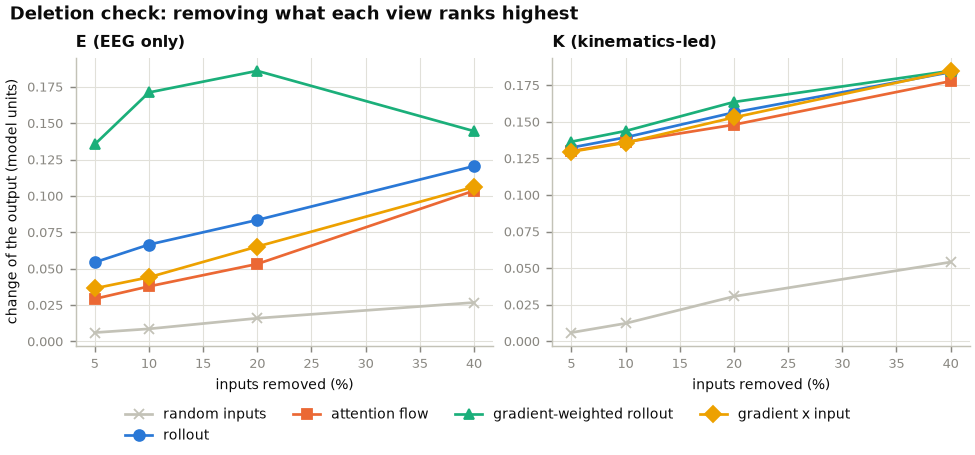
\includegraphics[width=0.40\textwidth,height=17mm,keepaspectratio]{P2_deletion.png}}
  \FigCap{Left: lift-off minus rest (occipital higher in all muscles). Right: deletion curves.}
\end{frame}

\begin{frame}{Appendix: attention flow of all participants}
  \FigRow{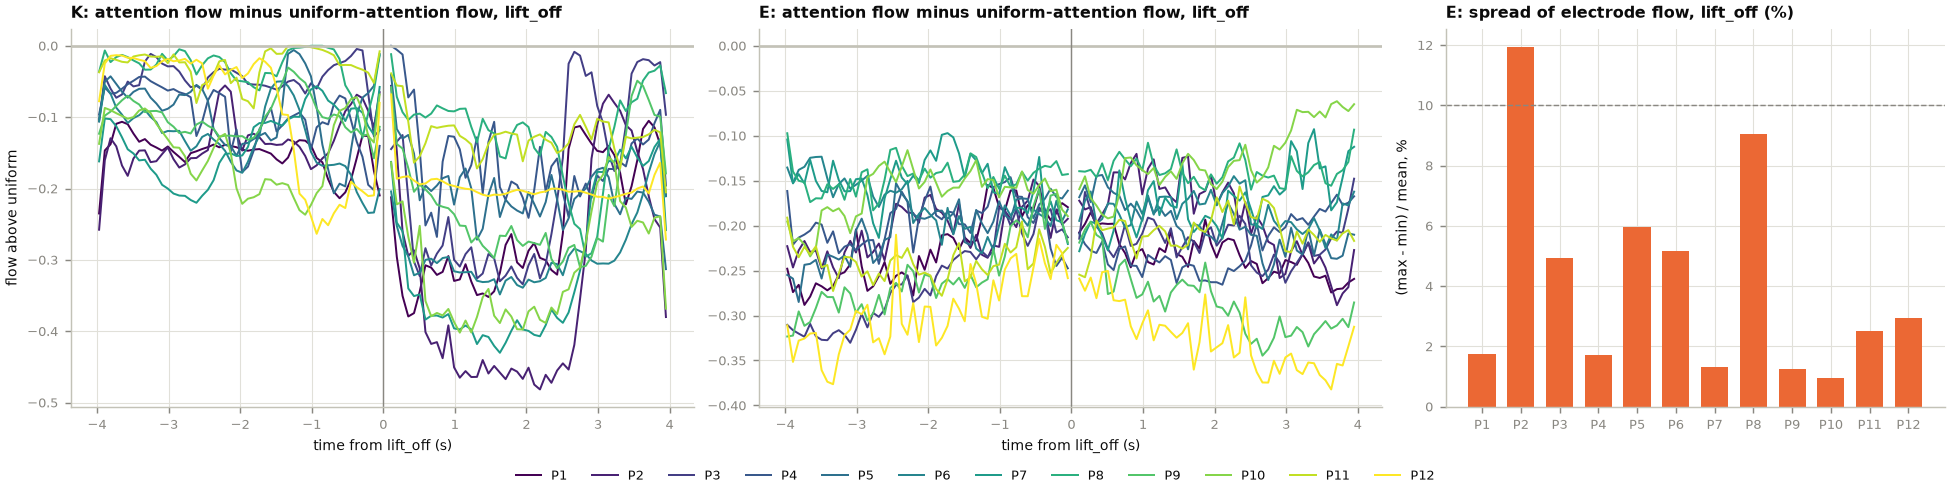
\includegraphics[width=\textwidth,height=32mm,keepaspectratio]{flow_all.png}}
  \FigCap{Flow minus uniform-attention flow around lift-off for K (left) and E (middle), one line per participant.
          Right: spread of E's electrode flow; below the 10\% line a map is not informative.}
  \vspace{2mm}
  \FigRow{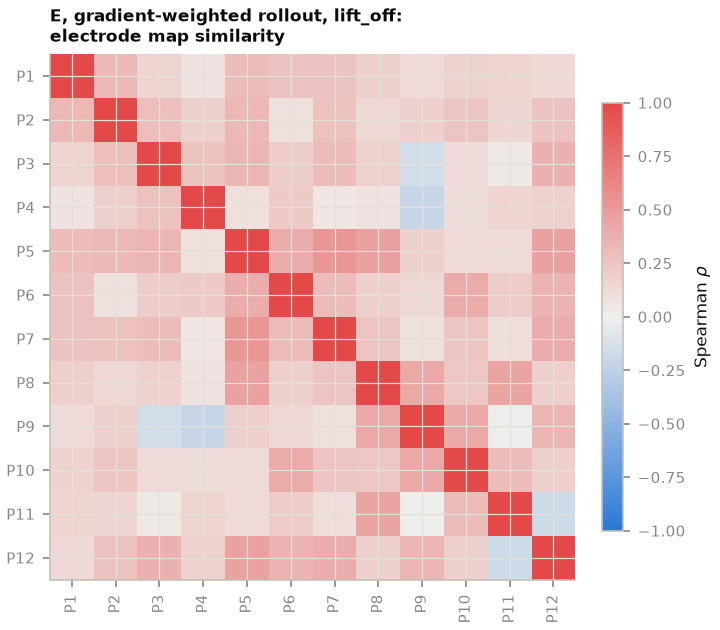
\includegraphics[height=28mm,keepaspectratio]{cons_similarity.png}\hspace{6mm}%
          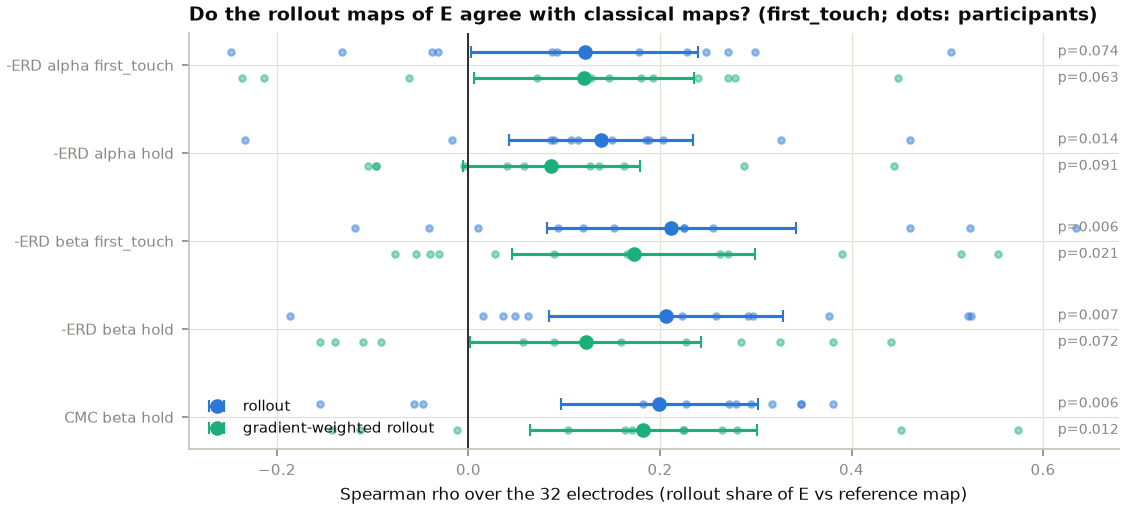
\includegraphics[width=0.5\textwidth,height=28mm,keepaspectratio]{ctrl_B4_rollout_vs_reference_first_touch.png}}
  \FigCap{Left: Spearman $\rho$ of E's electrode maps between every pair of participants. Right: Control B at first touch.}
\end{frame}

\end{document}
